\documentclass[11pt,a4paper]{article}

\def\nyear {2025}
\def\nterm {Spring}
\def\nlecturer {Chen Meiri}
\def\ncourse {Field Theory}

\makeatletter

% packages
\usepackage{amssymb,amsfonts,amsmath,calc,tikz,pgfplots,geometry,mathtools}
\usepackage{color}   % May be necessary if you want to color links
\usepackage[svgnames]{xcolor}
\usepackage[hidelinks]{hyperref}
\usepackage{forest}
\usepackage{commath} % ew
\usepackage{esvect} % \vv makes vectors
\usepackage{centernot} % for the comparison
\usepackage{esdiff}
\usepackage{esint}
\usepackage{amsthm}
\usepackage{fancyhdr}
\usepackage{bm}
\usepackage{witharrows}
\usepackage{bookmark}
\usepackage{tikz-cd}
\usepackage{quiver}
\usepackage{bbm}
\usepackage{textcomp}
\usepackage{float}
\usepackage{gensymb}
\usepackage{cleveref}
\usepackage{environ}
\usepackage{comment}
\usepackage{cancel}
\usepackage{xparse}

% Inevitable cs
\usepackage{listings}
\usepackage[]{algorithm2e}

% tikz libraries
\usetikzlibrary{positioning}
\usetikzlibrary{matrix}
\usetikzlibrary{arrows}
\usetikzlibrary{bending}
\usetikzlibrary{arrows.meta}
\usetikzlibrary{decorations.markings}
\usetikzlibrary{decorations.pathreplacing}
\usetikzlibrary{decorations.markings}
\usetikzlibrary{patterns}
\usetikzlibrary{backgrounds}

% Page style setup
\pagestyle{fancy}
\fancyhfoffset{0pt}
\renewcommand{\headwidth}{\textwidth}
\geometry{margin=1in}
\pgfplotsset{compat=1.18}
\setlength{\headheight}{14.6pt}
\addtolength{\topmargin}{-1.6pt}
\hypersetup{
    colorlinks=false,
    linktoc=section,
    linkcolor=black,
}

%% maketitle setup
\ifx \nauthor\undefined
  \def\nauthor{Yeheli Fomberg}
\else
\fi

\ifx \nemail\undefined
  \def\nemail{\href{mailto:yp@campus.technion.ac.il}
  {\texttt{<yp@campus.technion.ac.il>}}}
\else
\fi

\ifx \ncoursehead \undefined
  \def\ncoursehead{\ncourse}
\fi

\lhead{\emph{\nouppercase{\leftmark}}}
\ifx \nextra \undefined
  \rhead{
    \ifnum\thepage=1
    \else
      \ncoursehead
    \fi}
\else
  \rhead{
    \ifnum\thepage=1
    \else
      \ncoursehead \ (\nextra)
    \fi}
\fi

\def\notes{notes}
\def\problems{problems}

\ifx \ntype \undefined
  \def\ntype{notes}
\else
\fi

\ifx \ntype \notes
  \let\@real@maketitle\maketitle
  \renewcommand{\maketitle}{\@real@maketitle\begin{center}
  \begin{minipage}[c]{0.9\textwidth}\centering\footnotesize
  These notes are not endorsed by the lecturers.
  I have revised them outside lectures to incorporate supplementary
  explanations, clarifications, and material for fun.
  While I have strived for accuracy, any errors or misinterpretations 
  are most likely mine.
  \end{minipage}\end{center}}
\else
  \ifx \ntype \problems
    \let\@real@maketitle\maketitle
    \renewcommand{\maketitle}{\@real@maketitle\begin{center}
    \begin{minipage}[c]{0.9\textwidth}\centering\footnotesize
    These problems are mostly based on the problem sets I was given
    when taking the course.
    
    While I have strived for accuracy and completeness,
    some of the problems would not have been here without the help of
    friends.
    \end{minipage}\end{center}}
  \else
  \fi
\fi


% theorem environments
\theoremstyle{definition}
\newtheorem{definition}{Definition}[section]
\newtheorem{remark}{Remark}[section]
\newtheorem{example}{Example}[section]
\newtheorem{exercise}{Exercise}[section]
\newtheorem{paradox}{Paradox}[section]
\newtheorem{entry}{Entry}[section]
\newtheorem*{solution}{Solution}
\newtheorem*{question}{Question}
\newtheorem*{answer}{Answer}
\newtheorem*{problem}{Problem}
\theoremstyle{plain}
\newtheorem{theorem}{Theorem}[section]
\newtheorem{proposition}[theorem]{Proposition}
\newtheorem{lemma}[theorem]{Lemma}
\newtheorem{corollary}[theorem]{Corollary}
\newenvironment{proofof}[1]{%
    \renewcommand{\proofname}{Proof of #1}%
    \begin{proof}
}{%
    \end{proof}
}
% tikz customization
\pgfarrowsdeclarecombine{twolatex'}{twolatex'}{latex'}{latex'}{latex'}{latex'}
\tikzset{->/.style = {decoration={markings,
                                  mark=at position 0.999
                                  with {\arrow[scale=2]{latex'}}},
                      postaction={decorate}}}
\tikzset{<-/.style = {decoration={markings,
                                  mark=at position 0.001 with {\arrowreversed[scale=2]{latex'}}},
                      postaction={decorate}}}
\tikzset{-->/.style = {decoration={markings,
                                  mark=at position 0.999
                                  with {\arrow[scale=2]{latex'[sep=0pt -2.5]}}},
                      postaction={decorate}}}
\tikzset{<--/.style = {decoration={markings,
                                  mark=at position 0.001
                                  with {\arrowreversed[scale=2]{latex'[sep=0pt -2.5]}}},
                      postaction={decorate}}}
\tikzset{<->/.style = {decoration={markings,
                                  mark=at position 0.001 with {\arrowreversed[scale=2]{latex'}},
                                  mark=at position 0.999 with {\arrow[scale=2]{latex'}},},
                      postaction={decorate}}}
\tikzset{->-/.style = {decoration={markings,
    mark=at position 0.50+0.225/#1 with {\arrow[scale=2]{latex'}}},
                      postaction={decorate}}}
\tikzset{-<-/.style = {decoration={markings,
                                   mark=at position 0.50-0.225/#1 with {\arrowreversed[scale=2]{latex'}}},
                       postaction={decorate}}}
\tikzset{->>/.style = {decoration={markings,
                                  mark=at position 1 with {\arrow[scale=2]{latex'}}},
                      postaction={decorate}}}
\tikzset{<<-/.style = {decoration={markings,
                                  mark=at position 0 with {\arrowreversed[scale=2]{twolatex'}}},
                      postaction={decorate}}}
\tikzset{<<->>/.style = {decoration={markings,
                                   mark=at position 0 with {\arrowreversed[scale=2]{twolatex'}},
                                   mark=at position 1 with {\arrow[scale=2]{twolatex'}}},
                       postaction={decorate}}}
\tikzset{->>-/.style = {decoration={markings,
                                   mark=at position 0.50+0.450/#1 with {\arrow[scale=2]{twolatex'}}},
                       postaction={decorate}}}
\tikzset{-<<-/.style = {decoration={markings,
                                   mark=at position 0.50-0.450/#1 with {\arrowreversed[scale=2]{twolatex'}}},
                       postaction={decorate}}}

\pgfarrowsdeclare{biggertip}{biggertip}{%
  \setlength{\arrowsize}{1pt}
  \addtolength{\arrowsize}{.1\pgflinewidth}
  \pgfarrowsrightextend{0}
  \pgfarrowsleftextend{-5\arrowsize}
}{%
  \setlength{\arrowsize}{1pt}
  \addtolength{\arrowsize}{.1\pgflinewidth}
  \pgfpathmoveto{\pgfpoint{-5\arrowsize}{4\arrowsize}}
  \pgfpathlineto{\pgfpointorigin}
  \pgfpathlineto{\pgfpoint{-5\arrowsize}{-4\arrowsize}}
  \pgfusepathqstroke
}
\tikzset{
	EdgeStyle/.style = {>=biggertip}
}

\tikzset{circ/.style = {fill, circle, inner sep = 0, minimum size = 3}}
\tikzset{scirc/.style = {fill, circle, inner sep = 0, minimum size = 1.5}}
\tikzset{mstate/.style={circle, draw, black, text=black, minimum width=0.7cm}}

\tikzset{eqpic/.style={baseline={([yshift=-.5ex]current bounding box.center)}}}

\definecolor{mblue}{rgb}{0.2, 0.3, 0.8}
\definecolor{morange}{rgb}{1, 0.5, 0}
\definecolor{mgreen}{rgb}{0, 0.4, 0.2}
\definecolor{mred}{rgb}{0.5, 0, 0}

% topology
\DeclareMathOperator{\dfr}{dfr} % deformation retract
\newcommand{\Cells}{\text{Cells}}
\newcommand{\RP}{\mathbb{RP}}
\newcommand{\CP}{\mathbb{CP}}

% order theory
\newcommand{\join}{\vee}
\newcommand{\meet}{\wedge}

% algebraic geometry
\DeclareMathOperator{\Rad}{Rad} % Radical of modules
\DeclareMathOperator{\Spec}{Spec}
% \renewcommand{\div}{\mathrm{div}} % divisors
\DeclareMathOperator{\Mer}{Mer} % Meromorphic functions
\DeclareMathOperator{\Exc}{Exc} % Exceptional divisor
\DeclareMathOperator{\Td}{Td} % Todd classes

% algebra

\DeclareMathOperator{\trdeg}{tr.deg.}
\DeclareMathOperator{\odd}{odd}
\DeclareMathOperator{\even}{even}
\DeclareMathOperator{\lcm}{lcm}
\DeclareMathOperator{\ord}{ord}
\DeclareMathOperator{\codim}{codim}
\DeclareMathOperator{\Ann}{Ann}
\DeclareMathOperator{\Ext}{Ext}
\DeclareMathOperator{\Sym}{Sym}
\DeclareMathOperator{\Out}{Out}
\DeclareMathOperator{\Aut}{Aut}
\DeclareMathOperator{\End}{End}
\DeclareMathOperator{\Inn}{Inn}
\DeclareMathOperator{\Mat}{Mat}
\DeclareMathOperator{\Fix}{Fix}
\DeclareMathOperator{\std}{std}
\DeclareMathOperator{\sgn}{sgn}
\DeclareMathOperator{\adj}{adj}
\DeclareMathOperator{\id}{id}
\DeclareMathOperator{\op}{op}
\DeclareMathOperator{\tr}{tr}
\DeclareMathOperator{\diag}{diag}
\DeclareMathOperator{\rank}{rank}
\DeclareMathOperator{\rk}{rk}
\DeclareMathOperator{\coker}{coker}
\DeclareMathOperator{\Mult}{Mult} % multiplier algebra
\DeclareMathOperator{\Frac}{Frac} % fraction field
\DeclareMathOperator{\Rat}{Rat}
\DeclareMathOperator{\Gal}{Gal}
\newcommand{\ioplus}{\overset{\text{int}}{\oplus}} % interior direct sum
\newcommand{\GG}{\mathcal G} % Galois correspondence
\newcommand{\FF}{\mathcal F} % Galois correspondence
\newcommand{\cupp}{\smile} % cup product
\newcommand{\capp}{\frown} % cap product
\newcommand{\actson}{\curvearrowright}
\newcommand{\bra}{\left\langle}
\newcommand{\ket}{\right\rangle}
\newcommand{\idealin}{\triangleleft\,}
\newcommand{\normalin}{\triangleleft\,}
\newcommand{\ip}[2]{\left\langle #1, #2 \right\rangle}
\newcommand{\bigslant}[2]
{{\raisebox{.2em}{$#1$}\left/\raisebox{-.2em}{$#2$}\right.}}
\newcommand{\properideal}{%
  \mathrel{\ooalign{$\lneq$\cr\raise.22ex\hbox{$\lhd$}\cr}}}

% categories
\newcommand{\cat}[1]{\mathbf{#1}}
\newcommand{\Ch}{\cat{Ch}} % Chain complexes   
\newcommand{\Set}{\cat{Set}}
\newcommand{\Grp}{\cat{Grp}}
\newcommand{\Ab}{\cat{Ab}}
\newcommand{\Ring}{\cat{Ring}}
\newcommand{\CRing}{\cat{CRing}}
\newcommand{\Top}{\cat{Top}}
\newcommand{\Vect}{\cat{Vect}}
\newcommand{\cmod}{\cat{mod}}

%% matrix groups
\newcommand{\GL}{\mathrm{GL}}
\newcommand{\Or}{\mathrm{O}}
\newcommand{\PGL}{\mathrm{PGL}}
\newcommand{\PSL}{\mathrm{PSL}}
\newcommand{\PSO}{\mathrm{PSO}}
\newcommand{\PSU}{\mathrm{PSU}}
\newcommand{\SL}{\mathrm{SL}}
\newcommand{\msl}{\mathrm{sl}}
\newcommand{\SO}{\mathrm{SO}}
\newcommand{\Spin}{\mathrm{Spin}}
\newcommand{\Sp}{\mathrm{Sp}}
\newcommand{\SU}{\mathrm{SU}}
\newcommand{\U}{\mathrm{U}}
\let\char\relax
\newcommand{\char}{\text{char}}

% analysis
\renewcommand{\Re}{\mathrm{Re}}
\renewcommand{\Im}{\mathrm{Im}}
\NewDocumentCommand{\dx}{o}{
  \IfNoValueTF{#1}
    {\dif x}                  % if no optional argument
    {\dif^{#1} \!x}         % if optional argument
}
\NewDocumentCommand{\dy}{o}{
  \IfNoValueTF{#1}
    {\dif y}                  % if no optional argument
    {\dif^{#1} \!y}         % if optional argument
}
\newcommand{\dt}{\dif t}
\newcommand{\du}{\dif u}
\newcommand{\dv}{\dif v}
\newcommand{\dz}{\dif z}
\newcommand{\ds}{\dif s}
\newcommand{\dw}{\dif w}
\newcommand{\dr}{\dif r}
\newcommand{\dm}{\dif m}
\newcommand{\df}{\dif f}
\newcommand{\dV}{\dif V}
\newcommand{\dS}{\dif S}
\newcommand{\dA}{\dif \mathrm{A}}
\newcommand{\dmu}{\dif \mu}
\newcommand{\dnu}{\dif \nu}
\newcommand{\dtheta}{\dif \theta}
\newcommand{\domega}{\dif \omega}
\newcommand{\dsigma}{\dif \sigma}
\newcommand{\dtau}{\dif \tau}
\newcommand{\dvarphi}{\dif \varphi}
\renewcommand{\dif}{\mathrm{d}}
\renewcommand{\Dif}{\mathrm{D}}
\renewcommand{\triangle}{\Delta}
\newcommand{\ptriangle}{\partial \triangle}
\DeclareMathOperator{\im}{im}
\DeclareMathOperator{\cis}{cis}
\DeclareMathOperator{\rot}{rot}
\DeclareMathOperator{\vspan}{span}
\DeclareMathOperator{\grad}{grad}
\DeclareMathOperator{\curl}{curl}
\DeclareMathOperator{\esssup}{esssup}
\newcommand{\hodge}{{\mathnormal{\star}}}
\DeclareMathOperator{\range}{range}
\DeclareMathOperator{\Hom}{Hom}
\DeclareMathOperator{\Int}{Int}
\DeclareMathOperator{\Conv}{Conv} % convex hull
\newcommand{\ind}{\mathbbm{1}}
\DeclareMathOperator{\Res}{Res}
\DeclareMathOperator{\graph}{graph}
\DeclareMathOperator{\diam}{diam}
\DeclareMathOperator{\supp}{supp}
\DeclareMathOperator{\Vol}{Vol} % Volume
\DeclareMathOperator{\Area}{Area} % Area
\DeclareMathOperator{\area}{area}
\DeclareMathOperator{\Ind}{Ind} % Index
\newcommand{\length}{\mathrm{length}}

% logic
\DeclareMathOperator{\MOD}{MOD}
\DeclareMathOperator{\Theory}{Theory}
\newcommand{\notimplies}{%
  \mathrel{{\ooalign{\hidewidth$\not\phantom{=}$\hidewidth\cr$\implies$}}}}

% nice
\newcommand{\half}{\frac{1}{2}}
\newcommand{\pair}{\del}
\newcommand{\taking}[1]{\xrightarrow{#1}}
\newcommand{\otaking}[1]{\xleftarrow{#1}}
\newcommand{\inv}{^{-1}}
\newcommand{\ot}{\leftarrow}
\newcommand{\ninfty}{-\infty}
\newcommand{\pinfty}{+\infty}
\newcommand{\floor}[1]{\left\lfloor #1 \right\rfloor}
\newcommand{\ceil}[1]{\left\lceil #1 \right\rceil}
\newcommand{\viff}{\Big\Updownarrow} % vertical iff
\newcommand{\bmid}{\,\middle\vert\,} % big mid

% probability
\newcommand{\Prob}{\mathbf{P}}
\renewcommand{\vec}[1]{\boldsymbol{\mathbf{#1}}}
\DeclareMathOperator{\Bin}{Bin}
\DeclareMathOperator{\Geo}{Geo}
\DeclareMathOperator{\Poi}{Poi}
\DeclareMathOperator{\Exp}{Exp}
\DeclareMathOperator{\Var}{Var} % Variance
\DeclareMathOperator{\Cov}{Cov}

% special letters
\newcommand{\N}{\mathbb{N}}
\newcommand{\Z}{\mathbb{Z}}
\newcommand{\Q}{\mathbb{Q}}
\newcommand{\R}{\mathbb{R}}
\newcommand{\C}{\mathbb{C}}
\newcommand{\F}{\mathbb{F}}
\newcommand{\E}{\mathbf{E}}
\newcommand{\D}{\mathbb{D}}
\renewcommand{\H}{\mathbb{H}}
\newcommand{\ps}{\mathcal{P}}
\newcommand{\M}{\mathcal{M}}
\renewcommand{\L}{\mathcal{L}}
\renewcommand{\O}{\mathcal{O}}
\renewcommand{\U}{\mathcal{U}}
\newcommand{\Omicron}{O}
\newcommand{\powerset}{\mathcal{P}}

% text
\newcommand{\st}{\text{ s.t. }}
\newcommand{\tand}{\quad \text{and} \quad}
\newcommand{\tor}{\quad \text{or} \quad}
\newcommand{\stand}{\text{ and }}
\newcommand{\stor}{\text{ or }}
\renewcommand{\tt}[1]{\textnormal{\textbf{(#1).}}} %tt=theorem title GET RID OF

% title format
\title{\textbf{\ncourse}}

\ifx \ntype \notes
  \author{Notes taken by \nauthor\, \nemail \\ Based on lectures by \nlecturer}
  \date{\nterm\ \nyear}
\else
  \ifx \ntype \problems
    \author{These problems were solved by \nauthor \\ \nemail}
  \else
  \fi
\fi

\makeatother

\renewcommand{\Dif}{\mathrm{D}}
\setcounter{section}{-1}
\begin{document}
\maketitle

% Insert cool image here

\newpage
\tableofcontents
\newpage

\section{Introduction}

\begin{definition}[Finite field extension]
  Let $E$ and $F$ be fields.
  We say that $E / F$ is a finite field extension if
  \begin{enumerate}
    \item[(1)] $F \subseteq E$
    \item[(2)] $\dim_F(E) < \infty$
  \end{enumerate}
\end{definition}

\begin{remark}
  Under certain conditions the fundamental theorem of Galois theory
  says that there exists a bijection between
  $\set{F \subseteq L \subseteq E \mid L \text{ is a field}}$
  and the set of subgroups of the automorphism group
  $\Aut(E/F) := \set{\alpha \in \Aut(E) \mid \alpha\vert_F = \id_F}$.
\end{remark}

\begin{remark}
  We can apply this theory when considering straightedge and compass
  constructions.
\end{remark}

\begin{example}
  Given a set of points in the plane so that $(0,0) \in S$.
  We can
  \begin{enumerate}
    \item[(1)] construct an edge between any two points in $S$;
    \item[(2)] construct a circle with center $s \in S$.
  \end{enumerate}
  We can construct points in the following ways:
  \begin{enumerate}
    \item[(1)] intersection of two lines;
    \item[(2)] intersection of two circles;
    \item[(3)] intersection of a line and a circle.
  \end{enumerate}
  Each point that we can construct in a finite sequence of these steps
  is called a constructable point (from $S$).
\end{example}

\begin{question}
  Which points can be constructed from $S$?
\end{question}
\begin{remark}
  We will see that $(\sqrt{2},0)$ can be constructed from
  $S = \set{(0,0),(1,0)}$ but $(\sqrt[3]{2},0)$ cannot.
\end{remark}

\begin{remark}
  Let $F$ be a field a chararcteristic $0$.
  The roots of the polynomial $p(x) = x^2 + bx + c$ are given by
  \[
    x_{1,2} = \frac{-b \pm \sqrt{b^2 - 4c}}{2}.
  \]
  There exists a finite field extension so that
  \begin{enumerate}
    \item[(1)] $\dim_F(E) = 2$;
    \item[(2)] there exists $a \in E$ so that $E = F(a)$;
    \item[(3)] $a^2 \in E$.
    \item[(4)] the polynomial splits into linear factors over $E$.
      This means that the roots of $p(x)$ are in $E$.
  \end{enumerate}
  In fact $(1)$ follows from $(2)$ and $(3)$.
\end{remark}

\begin{remark}
  Let $F$ be a field with $\char(F) = 0$ and
  let $h$ be a polynomial of with $\deg(h) \le 4$.
  Then there exists a finite field extension $E/F$,
  elements $a_1,\dots,a_k \in E$ and
  natural number $m_1,\dots,m_k$ so that
  \begin{enumerate}
    \item[(1)] $h(x)$ splits into linear factors over $E$;
    \item[(2)] $E = F(a_1,\dots,a_k)$;
    \item[(3)] for all $1 \le k \le i$ we have $a_i^{m_i} \in F$.
  \end{enumerate}
  We will show that if $\deg(h) \geq 5$ then this property does not
  hold always.
\end{remark}

\newpage

\section{Field extensions and basic definitions}
\subsection{The field}

\begin{definition}[Field]
  A field is triplet $(F,+,*)$ so that 
  \begin{enumerate}
    \item[(1)] $(F,+)$ is an abelian group, its unit is denoted by $0_F$;
    \item[(2)] $(F\setminus\set{0},*)$ is a group, its unit is denoted by $1_F$;
    \item[(3)] the distributive property hold.
      For any $a,b,c \in F$ we have
      \[
        a(b + c) = ab + ac.
      \]
  \end{enumerate}
  Equivalently, a field is a commutative ring with unit where every nonzero
  element is a unit.
\end{definition}

\begin{remark}
  Another equivalent definition for a field,
  is a commutative ring with unit $R$,
  such that its only proper ideal is the zero ideal.
\end{remark}

\begin{example}
  We have that $\Q \subseteq \R \subseteq \C$ and all of them are fields
  with the standard operations.
\end{example}

\begin{example}
  The set $\Q(i) = \set{x \in \C \mid \exists a,b \in \Q \st x = a + bi}$
  is a field with the induced operations from $\C$.
  It is clear that $\Q(i)$ is a commutative ring so we can see it is a field
  by showing that every nonzero element is invertible.
  Indeed if $a + bi \neq 0$ then
  \[
    a + bi \del{\frac{a}{a^2 + b^2} - \frac{b}{a^2+b^2} i} = 1
  \]
  which completes the proof.
\end{example}

\begin{example}
  Let $p$ be prime number.
  Then $F_p := \Z/(p)$ is a field with $p$ elements where $(p)$
  is the ideal generated by $p$.
  Moreover, it is the unique field with $p$ elements up to isomorphism.
\end{example}

\begin{example}
  Let $R$ be a commutative ring with unit
  and let $I \idealin R$.
  Then $R/I$ is a field if and only if $I$ is a maximal ideal.
\end{example}

\begin{example}
  Let $R$ be an integral domain.
  Then there exists a field $R \subseteq F$ so that $x \in F$ is of the
  form $\frac{a}{b}$ for $a,b \in R$ and $F$ is called the field
  of fractions of $R$.
\end{example}

\begin{definition}[Characteristic of a field]
  Let $F$ be a field.
  The characteristic of $F$ denoted $\char(F)$ is defined to be the order
  of $1_F$ in the abelian group $(F,+)$ if the order is finite,
  or $0$ if it is infinite.
\end{definition}

\begin{example}
  We have that
  \begin{enumerate}
    \item[(1)] $\char(\Q) = \char(\R) = \char(\C) = 0$;
    \item[(2)] $\char(F_p) = p$.
  \end{enumerate}
\end{example}

\begin{exercise}
  Let $F$ be a field.
  Show that $\char(F)$ is either $0$ or a prime number.
\end{exercise}
\begin{solution}
  Assume that $\char(F) \neq 0$.
  It suffices to show that $\char(F)$ is a prime number.
  By definition $\char(F) < \infty$ and we may denote $\char(F) = m$.
  Suppose next that $m = n_1 n_2$ for two natural numbers $n_1,n_2 \in \Z_+$.
  We now have that $0 = \char(F) = n_1 n_2$ and since $F$ is a field
  it is in particular an integral domain and thus $n_1 = 0$ or $n_2 = 0$.
  This is a contradiction which completes the proof.
\end{solution}

\begin{definition}[Subfield]
  Let $E$ be a field.
  A subset $F \subseteq E$ is called a subfield if it is a field
  under the induced $(+,*)$ operations.
\end{definition}

\begin{proposition}
  Let $E$ be a subfield of $F$.
  Then $0_E = 0_F$ and $1_E = 1_F$ and $\char(E) = \char(F)$.
\end{proposition}

\begin{definition}[Generated subfield]
  Let $F$ be a field and let $S \subseteq F$.
  The subfield generated by $S$ is the intersection of all subsets of $F$
  that contain $S$.
  This intersection is not empty since $S \subseteq F$ and it is a field
  since an intersection of fields is a field.
\end{definition}

\begin{definition}[Prime subfield]
  Let $F$ be a field.
  The prime subfield of $F$ is defined to be the subfield generated
  by $\set{1_F}$.
\end{definition}

\begin{remark}
  Field isomorphisms, homomorphisms and endomorphisms are defined the same
  way the are defined for fields.
  In particular we require $\varphi(1_{F_1}) = 1_{F_2}$ and thus
  homomorphisms of fields are always injections.
\end{remark}

\begin{exercise}
  Let $F$ be a field with $\char(F) = p$.
  Show that the prime subfield of $F$ is isomorphic to $F_p$.
  Moreover, show that if $\char(F) = 0$ then the prime subfield
  is isomorphic to $\Q$.
\end{exercise}
\begin{solution}
  Suppose that $\char(F) = p < \infty$.
  Define a map $\varphi \colon \Z \to F$ by
  $\varphi \colon 1 \mapsto 1_F$ and extended so that
  \[
    \varphi \colon n \mapsto \underbrace{1_F + \cdots + 1_F}_{n \text{ times}}.
  \]
  Then since $\char(F) = p$ we have that $\ker(\varphi) = p\Z$.
  Thus from the first isomorphism theorem
  \[
    F_p := \Z/p\Z \cong \im(\varphi) \subseteq F.
  \]
  Since $F_p \cong \im(\varphi)$ we obtain that $\im(\varphi)$ is a subfield
  of $F$.
  Since its generated by $1$, it is by definition the prime subfield of $F$,
  which completes this part of the proof.
  
  Next suppose that $\char(F) = 0$.
  Let $P$ denote the prime subfield of $F$.
  Construct a similar homomorphism
  $\varphi \colon P \to \Q$ with $\varphi(1_F) = 1$
  and extend the map so that it preserves addition and the inverse operation.
  Any homomorphism of fields is injective, and thus $\varphi$ is injective.
  Since for any $\frac{a}{b} \in \Q$ we have
  \[
    \varphi\del[4]{\frac{\overbrace{1_F + \cdots + 1_F}^{a \text{ times}}}{\underbrace{1_F + \cdots + 1_F}_{b \text{ times}}}} =
    \frac{\varphi\del[2]{\overbrace{1_F + \cdots + 1_F}^{a \text{ times}}}}{\varphi\del[2]{\underbrace{1_F + \cdots + 1_F}_{b \text{ times}}}} =
    \frac{a}{b}
  \]
  so it is clear that $\varphi$ is surjective.
  Thus $\varphi$ isomorphism which completes the proof.
\end{solution}

\subsection{Field extensions}
\begin{definition}[Field extension]
  Let $F$ and $E$ be fields.
  We say that $E$ is a field extension of $F$ and denote $E/F$ if
  $F \subset E$.
\end{definition}

\begin{proposition}
  Let $E/F$ be a field extension.
  Then $E$ is a vector space over $F$.
  In particular we have $+_F = +_E\vert_F$ and scalar multiplication
  is the restriction of $* \colon E \times E \to E$ to the set
  $F \times E$.
\end{proposition}

\begin{definition}[Degree of a field extension]
  Let $E/F$ be a field extension.
  The degree of $E/F$ is denoted $[E : F]$ and defined
  by $\dim_F(E)$.
  The extension is called a finite extension if $[E : F] < \infty$
  and otherwise an infinite extension.
\end{definition}
% exercise missing
\begin{example}
  We have that $[\C : \R] = 2$ and $[\R : \Q] = \infty$.
  The second follows from the fact $\Q$ is countable and thus any vector
  space of finite dimension over $\Q$ is countable.
\end{example}

\begin{theorem}
  \label{thm:basic-extension}
  Let $F$ be a field and let $h(x) \in F[x]$ be a nonconstant polynomial.
  Then there exists a field extension $E/F$ so that $h$ has a root
  in $E$ and $[E : F] \le \deg(h)$.
\end{theorem}
\begin{proof}
  Let $g(x)$ be an irreducable factor of $h(x)$.
  It suffices to find a field extension $E/F$ where $g(x)$ has a root
  and $[E : F] = \deg(g)$.

  Since $F[x]$ is a PID and $g(x)$ is irreducable then
  $\del{g(x)} \idealin F[x]$ is a maximal ideal.
  In particular $E := F[x]/\del{g(x)}$ is a field.
  Denote the quotient map $\rho \colon F[x] \to E$.
  The kernel of $\rho$ is $\del{g(x)}$ and in particular it doesn't
  contain any invertible elements.
  Thus $\rho\vert_F$ is an injection
  and then $\rho(F)$ is a subfield of $E$ which is isomorphic to $F$.
  We may assume that $F$ is a subfield of $E$ and $\rho\vert_F = \id_F$.
  We denote
  \[
    g(x) = a_n x^n + \cdots + a_0 \in F[x]
  \]
  where $a_n \neq 0$ and then
  \[
    g\del{\rho(x)} =
    a_n \rho(x)^n + \cdots + a_1 \rho(x) + a_0 =
    \rho\del{a_n x^n + \cdots + a_0} = \rho\del{g(x)} = 0.
  \]
  Thus $\rho(x) \in E$ is a root of $g$.
  We now need to show that $\rho(1),\rho(x),\dots,\rho(x^{n-1})$ is
  a basis of $E$ over $F$ where $n = \deg(g)$
  which will show that $[E : F] = \deg(g)$.

  Let $d(x) \in F[x]$.
  There exist $r,s \in F[x]$ so that $\deg(r) < n$ and
  \[
    d(x) = s(x)g(x) + r(x)
  \]
  and so we get that
  \[
    \rho\del{d(x)} =
    \rho\del{r(x)} \in \vspan_F\set{\rho(1),\dots,\rho(x^{n-1})}
  \]
  and in particular $\set{\rho(1),\dots,\rho(x^{n-1})}$ spans $E$ as
  a vector space over $F$.
  These elements are also linearly independent since if
  $b_0,\dots,b_{n-1} \in F$ and
  \[
    b_0 \rho(0) + \cdots b_{n-1} \rho(x^{n-1}) = 0
  \]
  then
  \[
    \rho(b_0 + \cdots + b_{n-1} x^{n-1}) = 0
  \]
  which implies that $b_0 + \cdots + b_{n-1} x^{n-1} \in \del{g(x)}$
  but this is not possible since all the polynomials in $\del{g(x)}$
  are of degree greater or equal to $n$, which completes the proof.
\end{proof}

\begin{theorem}
  Let $F \subseteq E \subseteq K$ be fields.
  Then $[K : F] = [K : E] [E : F]$.
\end{theorem}
\begin{proof}
  Assume that $[E : F] = \infty$ or $[K : E] = \infty$ then
  obviously $[K : F] = \infty$.
  Assume now that $[E : F] = m$ and $[K : E] = n$ are finite.
  Let $\alpha_1,\dots,a_{m}$ be a basis of $E$ over $F$ and
  $\beta_1,\dots,\beta_{n}$ be a basis of $K$ over $E$.
  It suffices to show that the sequence
  \[
    (a_i b_j)_{\substack{1 \le i \le m \\ 1 \le j \le n}}
  \]
  is a basis of $K$ over $F$, which follows from linear algebra arguments.
  % to be added
\end{proof}

\begin{definition}[Finitely generated field extension]
  Let $E/F$ be a field extension and let $S$ be a subset of $E$.
  We denote $F(S)$ the smallest subfield of $E$ generated by $S \cup F$.
  Suppose that $S = \set{a_1,\dots,a_n}$.
  We sometimes denote $F(a_1,\dots,a_n)$ instead of $F(S)$.
  We say that $E/F$ is finitely generated if there exists a finite
  $S \subseteq E$ so that $E = F(S)$.
\end{definition}

\begin{exercise}
  Let $E/F$ be a field extension and let
  $S = \set{\alpha_1,\dots,\alpha_n} \subseteq F$.
  Show that
  \[
    F(S) = \set{\frac{p(s_1,\dots,s_n)}{q(s_1,\dots,s_n)} \,\middle\vert\,
    p,q \in F[s_1,\dots,s_n] \stand q \neq 0}.
  \] 
\end{exercise}

\subsection{Algebraic extensions}
\begin{definition}[Algebraic element]
  Let $E/F$ be a field extension and let $\alpha \in E$.
  We say that $\alpha$ is algebraic over $F$ if there exists a polynomial
  $g(x) \neq 0$ with coeffcients in $F$ so that $g(\alpha) = 0$.
\end{definition}
\begin{definition}[Transcendental number]
  Let $E/F$ be a field extension and let $\alpha \in E$.
  We say that $\alpha$ is transcendental if it is not algebraic.
\end{definition}

\begin{remark}
  Since a polynomial of degree $n$ there exist at most $n$ roots
  and $\Q[x]$ is countable, there exist at most a countable amount
  of algebraic numbers of any field extension over $\Q[x]$
  and in particular $\C$ contains transcendental numbers over $\Q$.
\end{remark}

\begin{definition}[Liouville number]
  An irrational real number $x$ is said to be a Liouville number if
  for every integer $n \geq 1$ there exist integers $p$ and $q \geq 2$ 
  so that $\abs{x - \frac{p}{q}} < \frac{1}{q^n}$.
\end{definition}

\begin{theorem}[Liouville's theorem]
  \label{thm:liouville}
  Liouville numbers are transcendental.
\end{theorem}
\begin{proof}
  Let $x$ be a Liouville number.
  Assume by contradiction that $x$ is an algebraic number.
  Since $x$ is a Liouville number, it is irrational
  so by a theorem not shown here
  there exists $c > 0$ and $n \in \Z_+$ so that
  \[
    \abs{x - \frac{p}{q}} \geq \frac{c}{q^n}
  \]
  for every pair $p,q \in \Z$ with $q \neq 0$.
  Let $r \geq 1$ so that $2^{r} \geq c^{-1}$.
  Since $x$ is a Liouville number there exist $p,q \in \Z$ with $q > 1$
  so that
  \begin{align*}
    \abs{x - \frac{p}{q}} < \frac{1}{q^{n+1}}
                          \le \frac{1}{2^r q^n}
                          \le \frac{c}{q^n}
  \end{align*}
  which is a contradiction.
  Thus $x$ is transcendental.
\end{proof}

\begin{exercise}
  Show that Liouville's constant 
  \[
    \alpha = \sum_{k=1}^{\infty} 10^{-k!}
  \]
  is transcendental over $\Q$.
\end{exercise}
\begin{solution}
  We can show that Liouville's constant is a Liouville' number
  and thus by \Cref{thm:liouville} it is transcendental.
\end{solution}

\begin{definition}[Minimal polynomial of an algebraic number]
  Let $E/F$ be a field extension and let $\alpha \in E$ be an algebraic number.
  The minimal polynomial of $\alpha$ over $F$ denoted $m_{\alpha}(x)$
  is the minimal monic polynomial with respect to degree in $F[x]$ that vanishes
  at $\alpha$.
\end{definition}
\begin{remark}[Degree of algebraic element]
  The degree of $m_{\alpha}(z)$ is called the degree of $\alpha$ over $F$
  and denoted by $\deg_F(\alpha)$ or $\deg(\alpha)$.
\end{remark}
\begin{remark}
  The minimal polynomial of $\alpha$ is unique and it generates the ideal
  \[
    \set{g(x) \in F[x] \mid g(\alpha) = 0} \idealin F[x].
  \]
  Assume that it is not unique, for example let $f$, $g$ be monic polynomials
  of degree $n$ that vanish at $\alpha$.
  Then $f - g$ is a polynomial of degree $< n$ that with root $\alpha$
  so there exists a monic polynomial of degree $< n$ which implies
  the uniqueness of the minimal polynomial.
\end{remark}

\begin{example}
  The minimal polynomial of $i \in \C$ over $\Q$ is $m_i(x) = x^2 + 1$.
\end{example}

\begin{proposition}
  Let $E/F$ be a fields extension,
  let $\alpha \in E$ and
  let $g(x) \in F[x]$ be a monic polynomial that vanishes at $\alpha$.
  Then $g(x)$ is the minimal polynomial of $\alpha$ over $F$ if and only
  if $g(x)$ is irreducable.
\end{proposition}
% to be added proof

\begin{theorem}[Eisenstein's criterion]
  \label{thm:eisensteins-criterion}
  Suppose we have the following polynomial with integer coefficients:
  \[
    Q(x) = a_{n} x^{n} + a_{n-1} x^{n-1} + \cdots + a_{1} x + a_{0}.
  \]
  If there exists a prime number $p$
  such that the following three conditions all apply:
  \begin{enumerate}
    \item[(1)] $p$ divides each $a_i$ for $0 \le i < n$;
    \item[(2)] $p$ does not divide $a_n$;
    \item[(3)] $p^2$ does not divide $a_0$;
  \end{enumerate}
  then $Q$ is irreducible over the rational numbers.
\end{theorem}

\begin{corollary}
  Let $p$ be a prime number.
  Then the polynomial
  \[
    g(x) = \frac{x^p - 1}{x - 1} = x^{p-1} + \cdots + x + 1 \in \Z[x].
  \]
  is irreducible over $\Q[x]$.
\end{corollary}
\begin{proof}
  We know that $f(x)$ is irreducible if and only if $f(x+1)$ is irreducible
  and indeed according to \Cref{thm:eisensteins-criterion} the polynomial
  \[
    g(x+1) =
    \frac{(x+1)^{p-1} - 1}{x} =
    \sum_{i=1}^{p} \binom{p}{i} x^{i-1}
  \]
  is irreducible.
\end{proof}

\begin{corollary}
  \label{cor:special-polynomial}
  Let $p$ be a prime number.
  Then the minimal polynomial of $e^{\frac{2 \pi i}{p}} \in \C$ over $\Q$
  is $x^{p-1} + x^{p-2} + \cdots + x + 1$.
\end{corollary}

\begin{proposition}
  Let $E/F$ be a field extension
  and let $\alpha \in E$ be algebraic over $F$.
  Then
  \begin{enumerate}
    \item[(1)] $F(\alpha) \cong F[x]/\del{m_{\alpha}(x)}$;
    \item[(2)] $[F(\alpha) : F] = \deg(\alpha)$.
  \end{enumerate}
\end{proposition}
\begin{proof} \phantom{}
\begin{enumerate}
  \item[(1)] Define a homomorphism of rings with unit
    \[
      \varphi \colon F[x] \to F(\alpha)
    \]
    by saying it is the identity on $F$ and setting $\varphi(x) = \alpha$.
    This homomorphism is the evaluation function at $\alpha$.
    In this way we have $\ker(\varphi) = \del{m_{\alpha}(x)}$
    and since $m_{\alpha}(x)$ is irreducible the ideal
    $\del{m_{\alpha}(x)}$ is maximal which implies that
    $F[x]/\del{m_{\alpha}(x)}$ is a field.
    From the first isomorphism theorem we get that $\varphi$ induces
    an isomorphism
    \[
      \overline \varphi \colon F[x]/\del{m_{\alpha}(x)}
      \taking{\cong} \im(\varphi) \subseteq F(\alpha).
    \]
    We have that $\im(\varphi)$ is a subfield of $F(\alpha)$ that
    contains $F$ and $\alpha$ and thus is equal to $F(\alpha)$.
  \item[(2)] This follows from $(1)$ since
    \[
      \deg_F F[x]/\del{m_{\alpha}(x)} = \deg\del{m_{\alpha}(x)}
    \]
\end{enumerate}
\end{proof}

\begin{corollary}
  Let $E/F$ be a field extension and let $\alpha$ be algebraic over $F$
  of degree $n$.
  Then $1,\alpha,\dots,\alpha^{n-1}$ is a basis of $F(\alpha)$ as a vector space
  over $F$.
\end{corollary}
\begin{proof}
  We will show that $1,\alpha,\dots,\alpha^{n-1}$ are linearly independent
  over $F$.
  Let $c_0,\dots,c_{n-1} \in F$ be such that
  \[
    c_0 1 + c_1 \alpha + \cdots + c_{n-1} \alpha_{n-1} = 0
  \]
  we can define a polynomial
  \[
    g(x) = c_0 + c_1 x + \cdots + c_{n-1} x^{n-1}
  \]
  and since $g(\alpha) = 0$ and $\deg(g) < \deg\del{m_{\alpha(x)}}$
  we get that $g(x)$ is the zero polynomial.

  Next since that $[F(\alpha) : F] = n$
  we have necessarily that $1,\alpha,\dots,\alpha^{n-1}$ is a basis
  which completes the proof.
\end{proof}

\begin{proposition}
  Let $E/F$ be a field extension and $\alpha \in F$.
  Then $\alpha$ is algebraic over $F$ if and only if
  $[F(\alpha) : F] < \infty$.
\end{proposition}
\begin{proof}
  We saw that if $\alpha$ is algebraic then
  $\left[F(\alpha) : F\right] = \deg(\alpha) < \infty$.

  Next suppose that $[F(\alpha) : F] < \infty$.
  Then $1,\alpha,\dots,\alpha^n$ are necessarily linearly dependent over $F$,
  which means that there exist $b_0,\dots,b_n \in F$ not all zero such that
  \[
    b_0 + b_1 \alpha + \cdots b_n \alpha^n = 0
  \]
  and thus $\alpha$ is a algebraic over $F$.
\end{proof}

\begin{definition}[Algebraic and transcendental extensions]
  Let $E/F$ be a field extension.
  \begin{enumerate}
    \item[(1)] We say that $E/F$ is an algebraic extension if every
      $x \in E$ is algebraic over $F$.
    \item[(2)] We say that $E/F$ is a transcendental extension
      if it is not an algebraic extension.
    \item[(3)] We say that $E/F$ is a pure transcendental extension if every
      $x \in E$ is transcendental over $F$.
  \end{enumerate}
\end{definition}

\begin{remark}
  The union of an increasing sequence of algebraic extensions 
  (with respect to containment) is algebraic.
\end{remark}

\begin{proposition}
  \label{prop:equal-three}
  Let $E/F$ be a field extension.
  Then the following conditions are equivalent:
  \begin{enumerate}
    \item[(1)] $E/F$ is finite;
    \item[(2)] $E/F$ is finitely generated and algebraic;
    \item[(3)] There exist alegbraic numbers $\alpha_1,\dots,\alpha_k \in E$
      over $F$ so that $E = F(\alpha_1,\dots,\alpha_k)$.
  \end{enumerate}
  Moreover, if $(3)$ is satisfied and for all $1 \le i \le n$ we have
  $m_i = \left[F(\alpha) : F\right]$ then we also have that
  $[E : F] \le m_1m_2 \cdots m_k$.
\end{proposition}
\begin{proof} \phantom{}
  \begin{enumerate}
    \item[($1 \to 2$)]
      Every finite extension is finitely generated
      (for example by the basis of $E$ over $F$).
      % to be added
    \item[($2 \to 3$)] Obvious.
    \item[($3 \to 1$)] For all $1 \le i \le k$ we denote
      \begin{enumerate}
        \item[(a)] $F_i = F(\alpha_1,\dots,\alpha_{i-i})$ and in particular
          $F_1 = F$;
        \item[(b)] $m_i = \left[F(\alpha_i) : F\right]$
          and $n_i = \left[F_i(\alpha_i) : F_i\right]$. 
      \end{enumerate}
      Since $m_i$ is the degree of the minimal polynomial of $\alpha_i$
      over $F$ and $n_i$ is the degree of the minimal polynomial
      over $\alpha_i$ over $F_i$, and
      since $F \subseteq F_i$, we get that $m_i \geq n_i$ for all
      $1 \le i \le n$.
      Thus we have
      \[
        [E : F] = [E : F_k] \cdot [F_k : F_{k-1}] \cdots [F_2 : F_1] =
        n_1 \cdots n_k \le m_1 \cdots m_k < \infty.
      \]
  \end{enumerate}
\end{proof}

\begin{corollary}
  Let $E/F$ be a field extension
  and let $\alpha,\beta \in E$ be algebraic over $F$ so that
  $\beta \neq 0$.
  Then $\alpha \pm \alpha$, $\alpha \beta$ and $\frac{\alpha}{\beta}$
  are all algebraic.
\end{corollary}
\begin{proof}
  The numbers $\alpha \pm \alpha$, $\alpha \beta$ and $\frac{\alpha}{\beta}$
  are all elements in $F(\alpha,\beta)$
  and by \Cref{prop:equal-three} we have that
  \[
    \left[F(\alpha,\beta) : F\right] \le \deg_F(\alpha) \deg_F(\beta),
  \]
  which completes the proof
\end{proof}

\begin{corollary}
  \label{cor:algebraic-closure-is-field}
  Let $E/F$ be a field extension.
  Then the collection of algebraic elements of $E$ over $F$
  is a subfield of $E$ that contains $F$.
\end{corollary}

\begin{exercise}
  Denote $\overline \Q$ the set of complex numbers that are
  algebraic over $\Q$.
  Show that $[\overline \Q : \Q] = \infty$.
  Also show that $[\R : \Q] = \infty$.
\end{exercise}

\begin{remark}
  By \Cref{cor:algebraic-closure-is-field}
  the set $\overline{\Q}$ is a field.
  It is sometimes called the algebraic closure of $\Q$.
\end{remark}

\begin{corollary}
  Let $E/F$ and $L/E$ be algebraic field extensions.
  Then $L/F$ is algebraic.
\end{corollary}
\begin{proof}
  Let $\alpha \in L$.
  It suffices to show that $\left[F(\alpha) : F\right] < \infty$.
  Let
  \[
    f(x) = x^n + a_{n-1} x^{n-1} + \cdots + a_1 x + a_0
  \]
  be the minimal polynomial of $\alpha$ over $E$.
  We denote $\set{a_{0},\dots,a_{n-1}} A \subseteq E$.
  Since $f$ is also the minimal polynomial of $\alpha$ over $F(A)$
  we have that $[F(\set{\alpha} \cup A) : F(A)] = n$.
  Thus we obtain
  \[
    \left[F(\alpha) : F\right] \le
    \left[F(\set{\alpha} \cup A) : F\right] =
    \underbrace{\left[F(\set{\alpha} \cup A) : F(A)\right]}_{=\,n}
    \underbrace{\left[F(A) : F\right]}_{<\,\infty} < \infty
  \]
  which completes the proof.
\end{proof}

\begin{definition}[Simple field extension]
  A field extension $E/F$ is called simple if there exists an element
  $\alpha \in E$ so that $E = F(\alpha)$.
  In this case we call $\alpha$ the primitive element of the extension.
\end{definition}

\begin{definition}
  Let $F$ be a field.
  The field of rational functions over $F$ is denoted by $F(x)$
  or equivalently the fraction field of $F[x]$.
\end{definition}

\begin{exercise}
  Let $E/F$ be a simple field extension.
  Show that one of the following is always satisfied.
  \begin{enumerate}
    \item[(1)] $E/F$ is a finite algebraic extension;
    \item[(2)] There exists an isomoprhism $\varphi \colon F(x) \to E$
      which is the identity on $F$.
  \end{enumerate}
\end{exercise}

\begin{exercise}
  Let $F(\alpha)/F$ be a simple field extension.
  Show that $F(\alpha)/F$ is finite if and only if $F(\alpha) = F[\alpha]$.
\end{exercise}

\subsection{The multiplicative group of a finite field}

\begin{lemma}
  \label{lem:abelian-groups}
  Let $G$ be a finite abelian group of order $n$.
  Suppose that $G$ is not cyclic.
  Then there exists $0 < m < n$ so that for all $g \in G$ we have
  $g^m = 1$.
\end{lemma}
\begin{proof}
  From the classification theorem for finitely generated abelian groups
  there exists a finite sequence of natural numbers
  $1 < m_1 \mid m_2 \mid \cdots \mid m_k$ so that
  \[
    G \cong C_{m_1} \times \cdots \times C_{m_k}.
  \]
  Since $G$ is not cyclic we get $k > 1$, and thus $|G| > m_k$.
  Since $g^{m_k} = 1$ for all $g \in G$ the proof is complete.
\end{proof}

\begin{corollary}
  \label{cor:multiplicative-group-of-finite-field-is-cyclic}
  Let $F$ be a field and let $G \leqslant F^{\times}$ be finite
  where $F^{\times}$ is the multiplicative group structure of the field.
  Then $G$ is cyclic, and in particular the multiplicative group structure
  of a finite field is cyclic.
\end{corollary}
\begin{proof}
  Assume by contradiction that $G$ is not cyclic and denote $|G| = n$.
  From \Cref{lem:abelian-groups} there exists $1 \le m < n$ so that
  $g^m = 1$ for all $g \in G$.
  This means that each polynomial $x^m - 1$ has $m < n$ differenet roots
  which is a contradiciton.
\end{proof}

\subsection{Algebraically closed fields}

\begin{definition}[Algebraically closed field]
  A field $F$ is said to be an algebraically closed field if each
  nonconstant polynomial $f \in F[x]$ has a root in $F$.
\end{definition}

\begin{proposition}
  Let $F$ be a field.
  The following conditions are equivalent:
  \begin{enumerate}
    \item[(1)] $F$ is an algebraically closed field;
    \item[(2)] every irreducible polynomial in $F[x]$ is of degree $1$;
    \item[(3)] every nonconstant monic polynomial $f \in F[x]$ splits into
      linear factors $f(x) = (x-\alpha_1)\cdots(x-\alpha_n)$ for
      $\alpha_1,\dots,\alpha_n \in F$.
  \end{enumerate}
\end{proposition}
\begin{proof} \phantom{}
  \begin{enumerate}
    \item[($1 \to 2$)] Let $f \in F[x]$.
      Suppose $f$ is constant,
      then it is either invertible or the zero polynoimal
      and thus it is not irreducible.
      Suppose $\deg f \geq 2$ then since $F$ is an algebraically closed field
      it has a root $\alpha \in F$ and thus $f(x) = (x - \alpha) g(x)$
      where $g(x) \in F[x]$ and $\deg g \geq 1$.
      In particular, $f$ is not irreducible which completes the proof.
    \item[($2 \to 3$)] Since every irreducible polynomial in $F[x]$ is
      of degree $1$ every polynomial $f(x)$ so that $\deg f \geq 2$
      can be written as a product of nonconstant polynomials of smaller
      degrees.
      Thus we can prove $(3)$ by induction on the degree of $f$.
    \item[($3 \to 1$)] Immediate.
  \end{enumerate}
\end{proof}

\begin{remark}
  We have already seen proofs for the
  fundamental theorem of algebra in other courses such as
  topology, and complex analysis, and thus we omitted the proof of this
  theorem in class.
  However, we will not omit its following two corollaries.
\end{remark}

\begin{corollary}
  Any real irreducible polynoimal $f \in \R[x]$ is of degree $\deg f \le 2$.
\end{corollary}
\begin{proof}
  Let $f \in \R[x]$ be irreducible.
  Let $\alpha \in \C$ be a root of $f$ as a polynomial in $\C[x]$.
  Then we have
  \[
    \deg f = \left[\R(\alpha) : \R\right] \le \left[\C : \R\right] = 2
  \]
  which completes the proof.
\end{proof}

\begin{corollary}
  Every real polynomial is a product of real polynomials of degree at most
  $2$.
  In particular, every real polynomial of an odd degree has a root.
\end{corollary}

\newpage

\section{Ruler and compass constructions}
\subsection{The system}
We start by setting $S = S_0 = \set{(0,0),(1,0)}$ which could be any two points
in the plane because they only serve as giving as the unit distance.

\begin{description}
  \item[Ruler:] Given two different points in $S$ we can draw
    a straight line between them of an arbitrary size.
  \item[Compass:] Given three points in $p,q,r \in S$
  so that $q \neq r$ we can draw the circle with center $p$ and
  radius $|r-q|$.
\end{description}
Denote by $S_1$ the set points given from the following types of intersections:
\begin{enumerate}
  \item[(1)] intersection of two constructible straight lines;
  \item[(2)] intersection of two constructible circles;
  \item[(3)] intersection of a constructible line and a constructible
    circle.
\end{enumerate}
The set $S_1$ is called the set of constructible points from $S_0$ in
one step.
For each $k \geq 1$ we denote $S_k$ the set of constructible points
from $S_{k-1}$ in one step.
We want to analyze the sets
\begin{enumerate}
  \item[(1)] $S_k$ and $T_{k} := \set{\abs{p - q} \mid p,q \in S_k}$;
  \item[(2)] $S_{\infty} := \bigcup_{k \geq 0} S_k$ and
    $T_{\infty} := \set{\abs{p - q} \mid p,q \in S_{\infty}}$;
  \item[(3)]
    $T_{\infty}^{\pm} := \set{x \in \R \mid \abs{x} \in T_{\infty}} =
    \set{x \in \R \mid (x,0) \in S_{\infty}}$.
\end{enumerate}

\subsection{Simple constructions}
\begin{remark}
  In the following constructions $0 := (0,0)$ always denotes the origin.
\end{remark}
\begin{remark}
  Although I have drawn the $x$-axis,
  I can't use it to create points without justification since this was not
  part of the rules.
  The justification is simple:
  every time we want to use the $x$-axis,
  we ``draw'' an infinite line segment passing through $(0,0)$ and $(1,0)$.
\end{remark}

\begin{example}
  \label{exmp:sum}
  Let $r,s \in T_{\infty}$.
  Then $r + s, |r - s| \in T_{\infty}$.
  Without loss of generality assume $0 < s \le r$.
  \begin{center}
    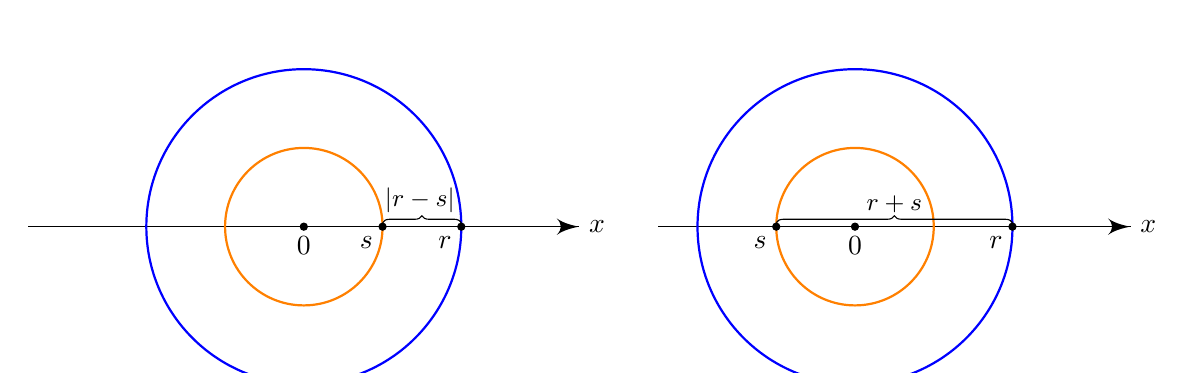
\begin{tikzpicture}[scale=1]
      % Draw x-axis
      \draw[->] (-7, 0) -- (0, 0) node[right] {$x$};
      \draw[->] (1, 0) -- (7, 0) node[right] {$x$};

      \draw[thick, orange] (3.5,0) circle (1);
      \draw[thick, blue] (3.5,0) circle (2);
      \fill (2.5,0) circle (1.5pt) node[below left] {$s$};
      \fill (5.5,0) circle (1.5pt) node[below left] {$r$};
      \fill (3.5,0) circle (1.5pt) node[below] {$0$};

      \draw[thick, orange] (-3.5,0) circle (1);
      \draw[thick, blue] (-3.5,0) circle (2);
      \fill (-2.5,0) circle (1.5pt) node[below left] {$s$};
      \fill (-1.5,0) circle (1.5pt) node[below left] {$r$};
      \fill (-3.5,0) circle (1.5pt) node[below] {$0$};

        \draw[decorate,decoration={brace}] (-2.5,0.05) -- (-1.5,0.05)
          node[midway,above] {{\small $\abs{r - s}$}};
        \draw[decorate,decoration={brace}] (2.5,0.05) -- (5.5,0.05)
          node[midway,above] {{\small $r+s$}};
    \end{tikzpicture}
  \end{center}
\end{example}
\begin{example}
  \label{exmp:division-by-two}
  Let $(x,0) \in S_{\infty}$.
  Then $(\half x,0) \in S_{\infty}$.
  \begin{center}
    \begin{tikzpicture}[scale=1]
      % Draw x-axis
      \draw[->] (-7, 0) -- (7, 0) node[right] {$x$};
      \draw[-,purple,thick] (0, 2.4) -- (0, -2.4);

      \draw[thick, orange] (-1,0) circle (2);
      \draw[thick, blue] (1,0) circle (2);
      \fill (-1,0) circle (1.5pt) node[below left] {$0$};
      \fill (1,0) circle (1.5pt) node[below left] {$x$};
      \fill (0,{sqrt(3)}) circle (1.5pt);
      \fill (0,{-sqrt(3)}) circle (1.5pt);
      \fill (0,0) circle (1.5pt) node[above left] {{\small $\half x$}};
    \end{tikzpicture}
  \end{center}
\end{example}
\begin{example}
  \label{exmp:lemma}
  Let $(x,y) \in S_{\infty}$.
  Then the line perpendicular to the $x$-axis that passes through $(x,y)$
  is constructible.
  
  Suppose $y = 0$ and then $(x,y) = (x,0)$.
  This case can either be shown directly
  or we can just you combine the results from 
  \Cref{exmp:sum} and \Cref{exmp:division-by-two}.
  \begin{center}
    \begin{tikzpicture}[scale=1]
      \draw[->] (-7, 0) -- (7, 0) node[right] {$x$};
      \draw[-,purple,thick] (0, 2.4) -- (0, -2.4);

      \draw[thick, orange] (-1,0) circle (2);
      \draw[thick, blue] (1,0) circle (2);
      \fill (-1,0) circle (1.5pt) node[below left] {$0$};
      \fill (1,0) circle (1.5pt) node[below right] {$x+x$};
      \fill (0,{sqrt(3)}) circle (1.5pt);
      \fill (0,{-sqrt(3)}) circle (1.5pt);
      \fill (0,0) circle (1.5pt) node[above left] {$x$};
    \end{tikzpicture}
  \end{center}
  In the general case we can draw a circle around $(x,y)$ with any radius
  greater than $y$, and then apply \Cref{exmp:division-by-two}
  on the two new points gained from the intersection with the $x$-axis.
  \begin{center}
    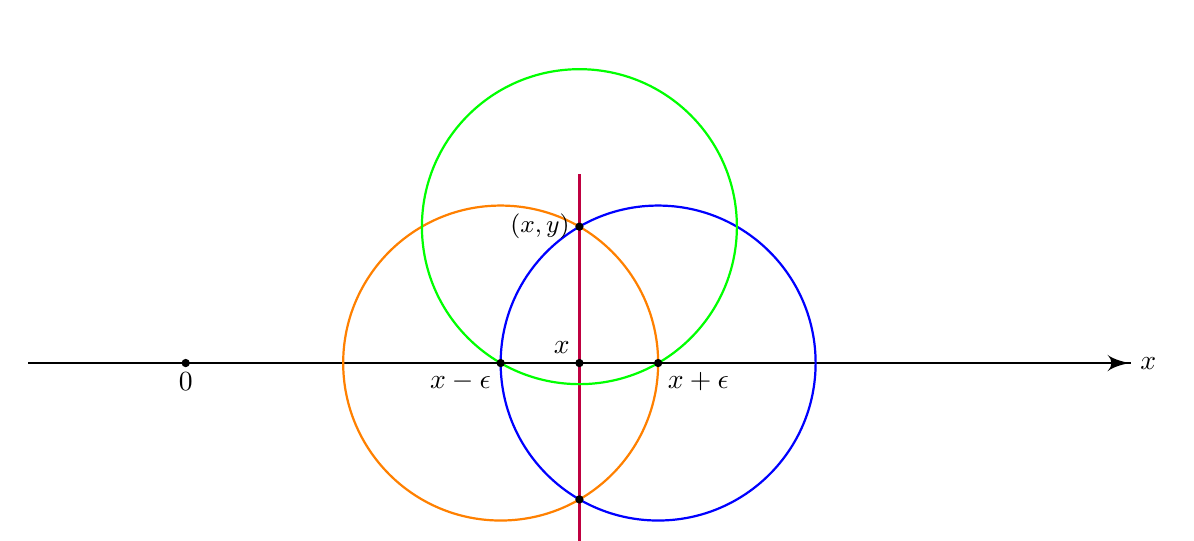
\begin{tikzpicture}[scale=1]
      \draw[->] (-7, 0) -- (7, 0) node[right] {$x$};
      \draw[-,purple,thick] (0, 2.4) -- (0, -2.4);

      \draw[thick, orange] (-1,0) circle (2);
      \draw[thick, blue] (1,0) circle (2);
      \draw[thick, green] (0,{sqrt(3)}) circle (2);
      \fill (-5,0) circle (1.5pt) node[below] {$0$};
      \fill (-1,0) circle (1.5pt) node[below left] {$x-\epsilon$};
      \fill (1,0) circle (1.5pt) node[below right] {$x+\epsilon$};
      \fill (0,{sqrt(3)}) circle (1.5pt) node[left] {{\small $(x,y)$}};
      \fill (0,{-sqrt(3)}) circle (1.5pt);
      \fill (0,0) circle (1.5pt) node[above left] {$x$};
    \end{tikzpicture}
  \end{center}
\end{example}

\begin{corollary}
  $S_{\infty} = T^{\pm}_{\infty} \times T^{\pm}_{\infty}$.
\end{corollary}
\begin{proof}
  This is an immediate corollary to \Cref{exmp:lemma} since
  any point $(x,y) \in S_{\infty}$ implies $(x,0),(0,y) \in S_{\infty}$
  and thus $x,y \in T_{\infty}^{\pm}$.
  The other side of the inclusion follows from a simple construction.
  Let $(x,y) \in T^{\pm}_{\infty} \times T^{\pm}_{\infty}$.
  Then $(x,0),(0,y) \in S_{\infty}$ and we can see that $(x,y) \in S_{\infty}$
  by noticing that it is the intersection of the circle of radius
  $|x-0|$ and center $y$ and the circle of radius $|y-0|$ and center $x$.
  \begin{center}
    \begin{tikzpicture}[scale=1]
      \draw[->] (-7, 0) -- (7, 0) node[right] {$x$};
      \draw[->] (0,-1.5) -- (0,3) node[right] {$y$};

      \draw[thick, orange] (1.5,0) circle (1);
      \draw[thick, blue] (0,1) circle (1.5);
      \fill (0,0) circle (1.5pt) node[above left] {$0$};
      \fill (0,1) circle (1.5pt) node[left] {$y$};
      \fill (1.5,0) circle (1.5pt) node[below] {$x$};
      \fill (1.5,1) circle (1.5pt) node[above right] {$(x,y)$};
    \end{tikzpicture}
  \end{center}
\end{proof}

\begin{example}
  \label{exmp:product-and-division}
  Let $s,r \in T_{\infty}$.
  Then $r s \in T_{\infty}$ and if $r \neq 0$
  then $\frac{s}{r} \in T_{\infty}$.
  We may assume that $s,r \neq 0$.
  From \Cref{exmp:sum} and \Cref{exmp:division-by-two} and \Cref{exmp:lemma}
  we know that the points $A = (0,0)$, $B = (1,0)$, $C = (1,s)$ and
  $D = (r,0)$ are construcible.
  We can now draw a line passing through $A$ and $C$ and a line
  perpendicular to the $x$-axis passing through $D$.
  We will denote their intersection point by $E$.
  The triangles $\triangle ABC$ and $\triangle ADE$ are similar, and so
  \[
    \frac{AB}{BC} = \frac{AD}{DE} \implies
    \frac{1}{s} = \frac{r}{DE} \implies DE = rs
  \]
  which completes the proof.
  Below is a diagram to visualize the process.
  \begin{center}
    \begin{tikzpicture}[scale=2.5]
      \draw[->] (-1,0) -- (5,0) node[right] {$x$};
      \draw[orange] (0,0) -- (4,2);
      \draw[blue] (4,0) -- (4,2);

      \fill (0,0) circle (1pt) node[below] {$0$};
      \fill (1,0) circle (1pt) node[below] {\small $(1,0)$};
      \fill (1,.5) circle (1pt) node[above left] {\small $(1,s)$};
      \fill (4,0) circle (1pt) node[below] {\small $(r,0)$};
      \fill (4,2) circle (1pt) node[right] {\small $(r,sr)$};

      \draw[decorate,decoration={brace,mirror}] (1+0.05/2,0) -- (1+0.05/2,.5)
        node[midway,right] {{\small $s$}};
      \draw[decorate,decoration={brace,mirror}] (4+0.05/2,0) -- (4+0.05/2,2)
        node[midway,right] {{\small $sr$}};
      \draw[decorate,decoration={brace,}] (0,0.05/2) -- (1,0.05/2)
        node[midway,above] {{\small $1$}};
      \draw[decorate,decoration={brace,mirror}] (0,-0.05/2) -- (4,-0.05/2)
        node[midway,below] {{\small $r$}};
      \draw[] node[above left] at (0,0) {A};
      \draw[] node[right] at (1,0.1) {B};
      \draw[] node[above right] at (1,0.55) {C};
      \draw[] node[right] at (4,0.1) {D};
      \draw[] node[left] at (4,2.05) {E};
    \end{tikzpicture}
  \end{center}
    In order to show that $\frac{s}{r} \in T_{\infty}$ we use a very
    similar construction
    \begin{center}
    \begin{tikzpicture}[scale=2.5]
      \draw[->] (-1,0) -- (5,0) node[right] {$x$};
      \draw[-,orange] (0,0) -- (4,2);
      \draw[-,blue] (4,0) -- (4,2);

      \fill (0,0) circle (1pt) node[below] {$0$};
      \fill (1,0) circle (1pt) node[below] {\small $(1,0)$};
      \fill (1,.5) circle (1pt) node[above left] {\small $(1,\frac{s}{r})$};
      \fill (4,0) circle (1pt) node[below] {\small $(r,0)$};
      \fill (4,2) circle (1pt) node[right] {\small $(r,s)$};

      \draw[decorate,decoration={brace,mirror}] (1+0.05/2,0) -- (1+0.05/2,.5)
        node[midway,right] {{\small $\frac{s}{r}$}};
      \draw[decorate,decoration={brace,mirror}] (4+0.05/2,0) -- (4+0.05/2,2)
        node[midway,right] {{\small $s$}};
      \draw[decorate,decoration={brace,}] (0,0.05/2) -- (1,0.05/2)
        node[midway,above] {{\small $1$}};
      \draw[decorate,decoration={brace,mirror}] (0,-0.05/2) -- (4,-0.05/2)
        node[midway,below] {{\small $r$}};
      \draw[] node[above left] at (0,0) {A};
      \draw[] node[right] at (1,0.1) {B};
      \draw[] node[above right] at (1,0.55) {C};
      \draw[] node[right] at (4,0.1) {D};
      \draw[] node[left] at (4,2.05) {E};
    \end{tikzpicture}
  \end{center}
  which completes the proof.
\end{example}

\begin{example}
  \label{exmp:square-root}
  Let $c \in T_{\infty}$.
  Then $\sqrt{c} \in T_{\infty}$.
  From the \Cref{exmp:product-and-division} we can assume that $r < 1$
  (we have already seen that if $1/t \in T_{\infty}$ then $t \in T_{\infty}$).
  We know from earlier examples that the point $(\frac{c+1}{2},0)$ can
  be constructed.
  We now construct the point $(1,y)$ by letting it be the intersection
  of the line perpendicular to the $x$-axis passing through $(1,0)$
  and the circle with radius $\frac{c+1}{2}$ and center $(\frac{c+1}{2},0)$.
  We can see this in the following diagram.
  \begin{center}
    \begin{tikzpicture}[scale=2.5]
      \draw[->] (-2,0) -- (2,0) node[right] {$x$};
      \draw[->] (0,-1) -- (0,1);
      \pgfmathsetmacro{\c}{0.4}
      \draw[thick, blue] ({(\c+1)/(2)},0) circle ({(\c+1)/(2)});
      \draw[thick,orange] (1,0) -- (1,{sqrt(\c)});

      \fill ({(\c+1)/(2)},0) circle (1pt) node[above] {\tiny$\del{\frac{c+1}{2},0}$};
      \fill (0,0) circle (1pt) node[above left] {$0$};
      \fill (1,0) circle (1pt) node[below] {\tiny$(1,0)$};
      \fill (1,{sqrt(\c)}) circle (1pt) node[above] {\tiny$(1,y)$};
    \end{tikzpicture}
  \end{center}
  This shows that $y$ is construcible and from the pythagorean theorem we
  have that
  \[
    y^2 + \del{1 - \frac{c+1}{2}} = \del{\frac{c+1}{2}}^2 \implies
    y^2 + 1 - (c + 1) + \del{\frac{c+1}{2}}^2 = \del{\frac{c+1}{2}}^2 \implies
    y = \sqrt{c}
  \]
  which completes the proof.
\end{example}

\begin{corollary}
  \label{cor:constructible-numbers-are-a-field}
  $T^{\pm}_{\infty}$ is a field.
\end{corollary}
\begin{proof}
  We have seen that $0,1 \in T_{\infty}^{\pm}$ and we have shown
  in examples
  that if $r,s \in T^{\pm}_{\infty}$ then $r \pm s, rs \in T^{\pm}_{\infty}$
  and if $r \neq 0$ that $s/r \in T^{\pm}_{\infty}$.
\end{proof}

\subsection{Lines and circles}

\begin{definition}[$F$-lines and $F$-circles]
  Let $F \subseteq \R$ be a field.
  \begin{enumerate}
    \item[(1)] A line $L \subset \R^2$ is called an $F$-line if its equation
    is $x = a$ or $y = ax + b$ for $a,b \in F$.
    \item[(2)] A circle $C \subseteq \R^2$ is called an $F$-circle if its
      equation is $(x - a)^2 + (y - b)^2 = c$ for $a,b,c \in F$.
  \end{enumerate}
\end{definition}
\begin{remark}
  Let $S_0 \subseteq F \times F$ for some field $F$.
  Then each point that is constructible from $S_0$ in one step
  is either an intersection of two $F$-lines,
  an intersection of $F$-circles
  or an intersection of an $F$-line and an $F$-circle.
\end{remark}

\begin{lemma}
  \label{lem:previous}
  Let $F \subseteq \R$ be a field,
  let $L_1 \neq L_2$ be $F$-lines
  and let $C_1 \neq C_2$ be $F$-circles.
  Then
  \begin{enumerate}
    \item[(1)] $L_1 \cap L_1 = \emptyset$ or they intersect at one point
      in $F \times F$.
    \item[(2)] $L_1 \cap C_1 = \emptyset$ or they intersect at two points
      or less and there exists $0 < \alpha \in F$ so that each intersection
      point is an element of $F(\sqrt \alpha) \times F(\sqrt \alpha)$.
    \item[(3)] $C_1 \cap C_2 = \emptyset$ or they intersect at two points
      or less and there exists $0 < \alpha \in F$ so that each intersection
      point is an element of $F(\sqrt \alpha) \times F(\sqrt \alpha)$.
  \end{enumerate}
\end{lemma}
\begin{proof}
  We are only going to prove case $(2)$ under the assumption that
  the equation of $L_1$ is $y = ax + b$ for $a,b \in F$.
  The equation of $C_1$ is $(x - c)^2 + (y - d)^2 = e$ for $c,d,e \in F$.
  In order to solve for the intersection points we need to substitute
  $y$ in $ax + b$ in the equation of the circle, and after some
  algebraic manipulations we see that intersection points must satisfy
  the equation
  \[
    (a^2 + 1) x^2 - 2(c + a(d - b))x =
    e - c^2 - (d - b)^2
  \]
  and so the intersection is nonempty if and only if this equation has
  a real solution, and in this case there exist $\alpha,\beta \in F$
  so that $0 \le \beta$ and the solutions are $\alpha \pm \sqrt{\beta}$.
  We conclude that
  \[
    x = \alpha \pm \sqrt{\beta} \in F\left(\sqrt \beta\right) \stand
    y = ax + b \in F\left(\sqrt \beta\right)
  \]
  which completes the proof.
\end{proof}

\begin{theorem}
  \label{thm:constructible-iff-tower-of-fields}
  Let $(0,0),(1,0) \in S_0 \subseteq \R^2$.
  We denote $F_0 := \Q(T_0)$.
  Then a real number $\alpha \in \R_{\geq 0}$ is constructible from $S_0$
  if and only if there exists a tower of fields
  $F_0 \subseteq F_1 \subseteq \cdots \subseteq F_k \subseteq \R$
  so that $\alpha \in F_k$ and for all $1 \le i \le k$
  there exists $0 \le \alpha_i \in F_{i-1}$ so that
  $F_i = F_{i-1}(\sqrt{\alpha_i})$.
\end{theorem}
\begin{proof}
  The previous lemma shows that this condition is necessary.
  \Cref{cor:constructible-numbers-are-a-field} shows that
  the constructible numbers are a field and \Cref{exmp:square-root}
  shows that if elements of a field $E \subseteq \R$ are constructible
  and $0 \le \alpha \in E$ then $\sqrt \alpha$ is constructible,
  and then from \Cref{cor:constructible-numbers-are-a-field} we
  have that $E(\sqrt \alpha)$ is a field.
  Thus we can use induction on $k$ to show that for every $1 \le i \le k$
  that the elements of $F_i$ are constructible which completes the proof.
\end{proof}
\begin{corollary}
  \label{cor:necessary-condition-for-constructability}
  Let $S_0 = \set{(0,0),(1,0)}$.
  Then a necessary condition for some $\alpha \in \R_{\geq 0}$ to be
  constructible is that $\left[\Q(\alpha) : \Q\right] = 2^k$
  for some $k \geq 0$.
\end{corollary}

\begin{remark}
  In this stage we still don't know that if $\alpha$ is constructible
  from $S_0 = F_0 \times F_0$ then there exists a tower of fields
  $F_0 \subseteq F_1 \subseteq \cdots \subseteq F_k = F(\alpha)$
  so that for all $1 \le i \le k$ we have $\left[F_i : F_{i-1}\right] = 2$
  but it is a corollary of \Cref{thm:constructible-iff-tower-of-fields}.
\end{remark}
% this is true tho ? we will see it later
\begin{remark}
  In later sections we will see a concrete example of some $\alpha \in \R$
  such that $\left[\Q(\alpha) : \Q\right] = 4$
  but $\alpha$ is not constructible from $S_0 = \set{(0,0),(1,0)}$.
\end{remark}

\begin{example}
  We know that $\pi$ is transcendental over $\Q$ and thus
  $\sqrt \pi$ is transcendental over $\Q$.
  This implies that we can't construct using a ruler and a compass
  a square with area $\pi$.
\end{example}

\begin{example}
  The polynomial $x^3 - 2$ is irreducible over $\Q$ by Eisenstein's
  criterion and thus it is the minimal polynomial of $\sqrt[3]{2} \in \R$.
  We get that $[\Q(\sqrt[3]{2}) : \Q] = 3$
  which shows that we can't draw the edge of a cube with volume $2$.
\end{example}

\begin{definition}[Fermat number]
  A Fermat number is a number of the form $F_{n}=2^{2^{n}}+1$,
  where $n$ is a positive integer.
\end{definition}

\begin{definition}[Fermat prime]
  Since if $2^k + 1$ is prime for a natural number $k > 0$
  it follows that $k$ itself is a power of two,
  any prime number of the form $2^k + 1$ is called a Fermat prime.
\end{definition}
\begin{remark}
  The only known Fermat primes are $3$, $5$, $17$, $257$ and $65537$.
  Moreover, it is unknown whether there are finitely or inifinitely many
  Fermat primes.
\end{remark}

\begin{example}
  \label{exmp:when-pgon-construcible-p-is-fermat}
  Let $p$ be an odd prime.
  We will show that if $\cos(2\pi/p)$ is constructible then $p$
  is a Fermat prime.
  We can see this by first denoting $\eta = e^{\alpha i}$
  and $\alpha = \frac{2\pi}{p}$.
  We have seen earlier in \Cref{cor:special-polynomial}
  that $\left[\Q(\eta) : \Q\right] = p - 1$.
  We see that
  \[
    \eta + \eta^{-1} =
    e^{\alpha i} + e^{-\alpha i} =
    2 \cos(\alpha) \implies
    \eta^2 - 2\cos(\alpha) \eta + 1 = 0
  \]
  which means that $\eta$ is a root of
  $x^2 - 2\cos(\alpha)x + 1 \in \Q(\cos(\alpha))$,
  and thus $\left[\Q(\eta) : \Q(\cos(\alpha))\right] \le 2$.
  On the other hand we have that $\Q(\cos(\alpha)) \subseteq \R$
  and since $\eta \notin \R$ that $\Q(\eta) \subsetneq \R$ so
  finally $\left[\Q(\eta) : \Q(\cos(\alpha))\right] = 2$.
  We have that
  \[
    \underbrace{\left[\Q(\eta) : \Q\right]}_{=\,p-1} =
    \underbrace{\left[\Q(\eta) : \Q(\cos(\alpha))\right]}_{=\,2}
    \left[\Q(\cos(\alpha)) : \Q\right]
  \]
  which implies that $\left[\Q(\cos \alpha) : \Q\right] = \frac{p-1}{2}$.
  Thus if $\cos(\alpha)$ is constructible then there exists $0 \le s$
  so that $\frac{p-1}{2} = 2^s$
  and thus $p = 2^{s+1} + 1$ which completes the proof.
\end{example}

\begin{remark}
  We will see later that the other direction of the proposition also holds.
  If $p$ is a Fermat prime then $\cos(2\pi/p)$ is constructible
  from $S_0 = \set{(0,0),(1,0)}$.
\end{remark}

\begin{exercise}
  Let $p$ be an odd prime.
  Show that $\cos(2\pi/p)$ is constructible if and only if
  it is possible to construct the vertices of a regular $p$-sided polygon,
  or equivalently, if and only if $p$ is a Fermat prime.
\end{exercise}

\newpage

\section{Introduction to Galois theory}
\subsection{Splitting fields}

\begin{definition}[Splitting over a field]
  Let $F$ be a field and let $g(x) \in F[x]$ be a polynomial of degree $n$.
  Then $g$ is said to split over $F$ if there exist
  $\alpha_1,\dots,\alpha_n \in F$
  not necessarily distinct so that
  \[
    g(x) = c (x - \alpha_1) (x - \alpha_2) \cdots (x - \alpha_n).
  \]
\end{definition}

\begin{definition}[Splitting field]
  \label{def:splitting-field}
  Let $F$ be a field and let $g(x) \in F[x]$ of degree $n$.
  A field extension $E/F$ is said to be a splitting field for $g$
  over $F$ if
  \begin{enumerate}
    \item[(1)] $g$ splits in $E$;
    \item[(2)] if $F \subseteq L \subsetneq E$ then $g$ does not split
      in $L$.
  \end{enumerate}
\end{definition}
\begin{remark}
  Condition $(2)$ in \Cref{def:splitting-field} means that $E$ is the minimal
  field where $g$ splits, with respect to containment of fields.
\end{remark}

\begin{remark}
  The splitting field of a polynomial is unique up to isomorphism.
\end{remark}

\begin{proposition}
  Let $F$ be a field and let $g(x) \in F[x]$ be a polynomial of degree $n$.
  Then there exists a field extension $E/F$ that is a splitting field
  of $g$ over $F$.
  Moreover, $[E : F] \le n!$.
\end{proposition}
\begin{proof}
  We will prove this by induction on $n$.
  When $n = 1$ then $g(x)$ is a linear polynomial and thus $F$
  is the splitting field of $g$ over $F$.
  Assume that $2 \le n$ and that the proposition holds for polynomials
  of degree less than $n$.

  Let $\alpha$ be a root of $g$.
  We have seen in \Cref{thm:basic-extension}
  that there exists a simple field extension $L/F$ so that
  $L = F(\alpha)$ and $[L : F] \le n$.
  We denote $h(x) = g(x) / (x - \alpha) \in L[x]$.
  From the induction hypothesis there exists a splitting field $E$ of $h$
  over $L$ and $[E : L] \le (n-1)!$,
  so we have that
  \[
    [E : F] = [E : L] [L : F] \le n!,
  \]
  and we want to show that $E$ is a splitting field of $g$ over $F$,
  so it is left to show that $E$ is the minimal field where $g$ splits.
  Assume, by way of contradiction,
  that $F \subseteq M \subsetneq E$ and $g$ splits in $M$.
  Then $M$ contains all the roots of $g$ and in particular $\alpha \in M$.
  Since $g$ splits over $M$, it follows that $h$ splits in $M$.
  From the previous two statements, and from the fact $E$ is the splitting
  field of $h$ over $L = F(\alpha)$ it follows that $E \subseteq M$.
  This contradiction completes the proof.
\end{proof}

\begin{example}
  \label{exmp:x-three-two}
  Let $f(x) = x^3 - 2 \in \Q[x]$.
  The roots of $f$ in $\C$ are $\alpha$, $\alpha w$, $\alpha w^2$
  where $\alpha = \sqrt[3]{2}$ and $w = e^{\frac{2 \pi i}{3}}$.
  Thus $\Q(\alpha,w)$ is the splitting field of $f$ over $\Q$.
  Notice that we have
  \[
    \left[\Q(\alpha,w) : \Q\right] =
    \left[\Q(\alpha,w) : \Q(\alpha)\right]
    \left[\Q(\alpha) : \Q\right].
  \]
  From Eisenstein's criterion we have that $f(x) = x^3 - 2$ is irreducible
  and is the minimal polynomial of $\alpha$ so
  $\left[\Q(\alpha) : \Q\right] = 3$.
  Since $w$ is a root of
  $\frac{x^3 - 1}{x - 1} = x^2 + x + 1 \in \Q(\alpha)[x]$
  we get that $\left[\Q(\alpha,w) : \Q(\alpha)\right] \le 2$
  so since clearly $w \notin \Q(\alpha)$ we get
  \[
    \left[\Q(\alpha,w) : \Q\right] =
    \underbrace{\left[\Q(\alpha,w) : \Q(\alpha)\right]}_{=\,2}
    \underbrace{\left[\Q(\alpha) : \Q\right]}_{=\,3} = 6.
  \]
\end{example}

\begin{definition}[Primitive $n$th root of unity]
  A primitive $n$th root of unity is a complex number $\zeta$
  satisfying $\zeta^n = 1$ and $\zeta^k \neq 1$ for all $1 \le k < n$.
\end{definition}
\begin{remark}
  Note that a primitive $n$th root of unity is not necessarily unique.
\end{remark}

\begin{example}
  Let $E/F$ be a field extension so that $E = F(\alpha)$ and let $\alpha$
  be a primitive $n$th root of unity.
  Then $\set{1,\alpha,\dots,\alpha^{n-1}}$ is the set of roots
  of the polynomial $x^n - 1$ and thus the splitting field of $x^n - 1$
  is $F(\alpha)$ and $[F(\alpha) : F] \le n$.
\end{example}

\begin{example}
  \label{exmp:splitting-field-prime}
  We know that for any prime $p \in \N$ we have for all $1 \le k \le p - 1$
  that $p \mid \binom{p}{k}$.
  This implies an identity that is colloquially known as
  the ``freshman's dream'' identity.
  It states that if $F$ is a field of prime characteristic $p$
  then for any $a,b \in F$ we get
  \[
    (a + b)^{p} = \sum_{i=0}^{p} \binom{p}{i} a^{i} b^{p-i} = a^p + b^p
  \]
  and in particular if $f(x) = x^p - a \in F[x]$ and $E = F(b)$
  is a simple field extension of $F$ where $b$ is a root of $f$,
  then $b^p = a$, and thus $f(x) = x^p - b^p = (x - b)^p$.
  This implies that $E$ is the splitting field of $f$.
\end{example}

\begin{exercise}
  \label{ex:show-x-p-irreducible}
  In example \Cref{exmp:splitting-field-prime}
  show that if $b \notin F$ then $f$ is irreducible over $F$
  and thus $[E : F] = p$.
\end{exercise}
% \begin{solution}
%   to be added.
% \end{solution}

\begin{definition}[Algebraic closure]
  Let $F$ be a field.
  An algebraic extension $E/F$ is said to be an algebraic closure of $F$
  if
  \begin{enumerate}
    \item[(1)] $E/F$ is algebraic;
    \item[(2)] $E$ is an algebraically closed field;
  \end{enumerate}
\end{definition}

\begin{exercise}
  Show that $(1) + (2)$ imply that if $F \subsetneq L \subsetneq E$ then $L$
  is not algebraically closed.
\end{exercise}

\begin{lemma}
  \label{lem:algebraic-closure}
  Let $E/F$ be an algebraic extension.
  Suppose that every $f(x) \in F[x]$ splits over $E$.
  Then $E$ is an algebraic closure of $F$.
\end{lemma}
\begin{proof}
  It suffices to show that $E$ is an algebraically closed field.
  Let $f(x) \in E[x]$ be a nonconstant polynomial.
  Let $L/E$ be an algebraic extension of $E$ so that $f$ has a root
  $\alpha \in L$.
  Since $L/E$ and $E/F$ are algebraic extensions,
  the extension $L/F$ is algebraic
  and in particular $\alpha$ is algebraic over $F$.
  Let $m(x) \in F[x]$ be the minimal polynomial of $\alpha$ over $F$,
  and let $h(x) \in E[x]$ be an irreducible element (over $E$) of $f(x)$
  so that $h(\alpha) = 0$.
  Then $h(x)$ is the minimal polynomial of $\alpha$ over $E$.
  This means that $h(x)$ divides $m(x)$.
  From the assumption we get that $m(x)$ splits over $E$
  and thus $h(x)$ also splits over $E$ and in particular $\alpha \in E$
  and $f(x)$ has a root in $E$.
\end{proof}

\begin{proposition}
  Let $F$ be a field.
  Then there exists an algebraic closure of $F$.
\end{proposition}
\begin{proof}
  Let $\set{f_{\alpha} \mid \alpha < \kappa}$ be an indexing of
  the elements of $F[x]$.
  We may assume that $\kappa$ is an infinite cardinal,
  and hence a limit ordinal.
  For all $\alpha \le \kappa$ we define an extension of $F$ in the following
  way:
  \begin{enumerate}
    \item[(1)] $F_0 = F$;
    \item[(2)] if $\alpha = \beta + 1$ is a successor ordinal then $F_{\alpha}$
      is the splitting field of $f_{\beta}$ over $F_{\beta}$;
    \item[(3)] if $\alpha$ is a limit ordinal then
      $F_{\alpha} = \bigcup\limits_{\beta < \alpha} F_{\beta}$;
  \end{enumerate}
  and we want to say that $F_{\kappa}$ is the algebraic closure of $F$.
  From \Cref{lem:algebraic-closure} it suffices to show that
  $F_{\kappa}/F$ is an algebraic extension.
  We will show by transfinite induction that for all $\alpha \le \kappa$
  the extension $F_{\alpha}/F$ is an algebraic extension.
  For the base $\alpha = 0$ it is clear that $F_{\alpha}/F = F/F$ is algebraic.
  Suppose that $\alpha$ is a successor ordinal so that $\alpha = \beta + 1$.
  From the induction hypothesis $F_{\beta}/F$ is algebraic.
  By definition of $F_{\alpha}$, $F_{\alpha}/F_{\beta}$ is algebraic.
  Thus $F_{\alpha}/F$ is algebraic.
  Suppose that $\alpha$ is a limit ordinal.
  Then $F_{\alpha}/F$ is algebraic since an increasing union of
  algebraic extensions is an algebraic extension.
  This completes the proof.
\end{proof}

\begin{lemma}
  \label{lem:simple-extension-isomorphism}
  Let $\sigma \colon E \to L$ be an isomorphism of fields.
  Let $f(x) = x^n + a_{n-1} x^{n-1} + \cdots + a_0 \in E[x]$ be irreducible,
  and denote
  $g(x) = \sigma(f) =  
    x^n + \sigma(a_{n-1}) x^{n-1} + \cdots + \sigma(a_0) \in L[x]$.
  Let $E(a) = \overline E$ and $L(b) = \overline L$ be field extensions
  so that $a$ is a root of $f$ and $b$ is a root of $g$.
  Then there exists a unique isomorphism
  $\overline \sigma \colon \overline E \to \overline L$ so that
  $\overline \sigma\vert_{E} = \sigma$ and $\overline \sigma(a) = b$.
  This could be summarized by the following commutative diagram:
  \[\begin{tikzcd}[ampersand replacement=\&,cramped]
    F \& {F(a)} \\
    L \& {L(b)}
    \arrow["{i_F}",hook, from=1-1, to=1-2]
    \arrow["\sigma"', from=1-1, to=2-1]
    \arrow["{\exists !\overline \sigma}", from=1-2, to=2-2]
    \arrow["{i_L}"',hook, from=2-1, to=2-2]
  \end{tikzcd}\]
\end{lemma}
\begin{proof} \phantom{}
  \begin{description}
    \item[Uniqueness:]
  We have that $\set{1,a,\dots,a^{n-1}}$ is a basis of $\overline E$
  over $E$ and thus $\overline \sigma\vert_E$ and $\overline \sigma(a)$
  uniquely determine $\overline \sigma$.
    \item[Existence:]
      There exist isomorphisms
      $\tau_1 \colon \overline E \to E[x]/\del{f(x)}$
      so that for every $e \in E$ we have $\tau_1(e) := e + \del{f(x)}$
      and $\tau_1(a) = x + \del{f(x)}$
      and $\tau_2 \colon \overline L \to L[x]/\del{g(x)}$ defined similarly.
      Also we define $\tau_3 \colon E[x]/\del{f(x)} \to L[x]/\del{g(x)}$
      by $h + \del{f(x)} \mapsto \sigma(h) + \del{g(x)}$.
      In this way we have that $\tau_2^{-1} \circ \tau_3 \circ \tau_1$
      is the desired isomorphism.
  \end{description}
\end{proof}

\begin{proposition}
  Let $F$ be a field.
  Let $E$ and $L$ be algebraic closures of $F$.
  Then there exists some isomorphism (not necessarily unique)
  $\rho \colon E \to L$ so that $\rho\vert_F = \id_F$.
\end{proposition}
\begin{proof}
  Let $\set{a_{\alpha} \mid \alpha < \kappa}$ where $\kappa$ is an infinite
  cardinal be an indexing of the elements of $E$.
  For all $\alpha \le \kappa$ we inductively define a field
  $F \subseteq F_{\alpha} \subset E$ in the following way:
  \begin{enumerate}
    \item[(1)] $F_0 := F$;
    \item[(2)] if $\alpha = \beta + 1$
      then $F_{\alpha} = F_{\beta}(\alpha_{\beta})$;
    \item[(3)] if $\alpha$ is a limit orindal then
      $F_{\alpha} = \bigcup\limits_{\beta < \alpha} F_{\beta}$.
  \end{enumerate}
  It is clear that $E = F_{\kappa}$.
  For every $\beta < \kappa$ we denote $m_{\beta}$ the minimal polynomial
  of $\alpha_{\beta}$ over $F_{\beta}$.
  Then $\deg m_{\beta} = \left[F_{\beta+1} : F_{\beta}\right]$.
  We can now define an embedding $\rho_{\alpha} \colon F_{\alpha} \to L$
  for every $\alpha \le \kappa$ so that for all $\beta \le \alpha \le \kappa$
  we have $\rho_{\alpha}\vert_{F_\beta} = \rho_{\beta}$
  (this means that $\rho_{\beta} \subseteq \rho_{\alpha}$).
  If $\rho_{\alpha}$ has already been defined
  then we denote $L_{\alpha} = \im(\rho_{\alpha})$.
  \begin{enumerate}
    \item[(1)] $\rho_0 = \id_F$;
    \item[(2)] if $\alpha = \beta + 1$ is a successor ordinal then
      since $L$ is algebraically closed we can choose $b_{\beta} \in L$
      which is the root of the irreducible polynomial
      $\rho_{\beta}(m_{\beta}) \in L_{\beta}[x]$ (it is irreducible
      since $\rho_{\beta}\vert_{F_{\beta}}$
      is an isomorphism and $m_{\beta}$ is irreducible).
      From \Cref{lem:simple-extension-isomorphism},
      there exists a unique extension of $\rho_{\beta}$ to an isomorphism
      \[
        \rho_{\alpha} \colon
        F_{\alpha} = F_{\beta}(a_{\beta}) \to L_{\beta}(b_{\beta}) \subseteq L
      \]
      so that $\rho_{\alpha}(a_{\beta}) = b_{\beta}$;
    \item[(3)] if $\alpha$ is a limit ordinal then
      we let $\rho_{\alpha} = \bigcup\limits_{\beta < \alpha} \rho_{\beta}$.
  \end{enumerate}
  Denote $\rho := \rho_{\kappa}$.
  We get that $\rho \colon F_{\kappa} = E \to L$
  is an embedding of $E$ in $L$ so that $\rho\vert_{F} = \id_F$,
  which also respects the field operations.
  It is left to show that $\rho$ is surjective.
  Let $b \in L$ and let $g$ be the minimal polynomial of $b$ over $\rho(E)$.
  We have that $\rho^{-1}(g)$ (we map $x$ to $x$) splits over $E$
  (since $E$ is algebraically closed),
  and thus $g$ splits over $\rho(E)$ and in particular $b \in \rho(E)$.
\end{proof}

\begin{exercise}
  Let $\sigma \colon F \to E$ be an isomorphism of fields.
  Let $g(x) \in F[x]$ and $h(x) = \sigma(g) \in E[x]$.
  Let $L/F$ and $M/E$ be the splitting fields of $g$ and $f$.
  Then $\sigma$ extends (not uniquely) to an isomorphism
  $\overline \sigma \colon M \to L$.
\end{exercise}
% \begin{solution}
%   to be added
%   % solution available in notes
% \end{solution}

\begin{corollary}
  \label{cor:splitting-fields-isomorphism}
  Let $F$ be a field.
  Let $E/F$ and $L/F$ be splitting fields
  of the same polynomial $f \in F[x]$.
  Then there exists an isomorphism $\sigma \colon E \to L$
  so that $\sigma\vert_F = \id_F$.
\end{corollary}

\begin{remark}
  Let $p \in \N$ be prime and let $E$ be a finite field of size $p^n$.
  Then the set $F = \set{0,1,2,\dots,p-1} \subseteq E$ is a subfield
  of $F$, and there exists a unique isomorphism
  $\rho \colon \Z/p\Z = F_{p} \to F$.
\end{remark}

\begin{lemma}
  Let $p$ be prime.
  Let $E$ be a field with $p^n$ elements and identify $F_p$ as
  a subfield of $E$.
  Then $E$ is the splitting field (over $F_p$) of the polynomial
  $x^{p^n} - x \in F_p[x]$.
\end{lemma}
\begin{proof}
  The multiplicative group $E^{\times}$ is of size $p^n - 1$,
  and thus from Cauchy's theorem for all $a \in E^{\times}$ we have
  $a^{p^n-1} = 1$.
  Since we also have that $0^{p^n-1} = 0$ it follows that all elements
  of $E$ are roots of the polynomial $x(x^{p^n-1} - 1) = x^{p^n} - x \in F[x]$.
  Since $|E| = p^n$, and a polynomial of degree $m$ has at most
  $m$ roots, it follows that $x^{p^n} - x$ splits over $E$.
  We get that $E$ is the splitting field
  of $x^{p^n} - x$ over $F_p$ which completes the proof.
\end{proof}

\begin{corollary}
  Let $p \in \N$ be prime and $1 \le n \in \N$.
  Then every two fields of order $p^n$ are isomorphic.
\end{corollary}
\begin{proof}
  The two fields are both splitting fields of $x^{p^n} - x$ over $F_p$,
  which is embedded uniquely in both of them.
  The result now follows directly from \Cref{cor:splitting-fields-isomorphism}.
\end{proof}

\begin{remark}
  This shows that any field of size $p^n$ is unique.
  In the next section we will show that there exists a field of size $p^n$
  for any prime $p$ and natural number $n \geq 1$.
\end{remark}

\subsection{The automorphism group of a field}
\begin{definition}[Automorphism group]
  Let $L$ be a field.
  The automorphism group of $L$ is given by
  \[
    \Aut(L) :=
    \set{\sigma \colon L \to L \mid \sigma \text{ is an isomorphism}}
  \]
  with the group operation being function composition.
\end{definition}

\begin{example}
  We will show that $\Aut(\Q) = \set{\id_{\Q}}$.
  Let $\sigma \in \Aut(\Q)$.
  We must have $\sigma(0) = 0$ and $\sigma(1) = 1$ and thus for any $n \in \N$
  \[
    \sigma(n) =
    \sigma(\underbrace{1 + 1 + \cdots + 1}_{n \text{ times}}) =
    \underbrace{\sigma(1) + \cdots \sigma(1)}_{n \text{ times}} =
    \underbrace{1 + 1 + \cdots + 1}_{n \text{ times}} = n,
  \]
  and from other properties of isomorphisms we get
  $\sigma(-n) = - \sigma(n) = -n$.
  From this follows that for any $a/b \in \Q$ we have
  $\sigma(a/b) = \sigma(a)/\sigma(b) = a/b$,
  which implies that $\sigma = \id_{\Q}$.
\end{example}

\begin{example}
  Let $p \in \N$ be a prime number.
  Then $\Aut(F_p) = \{\id_{F_p}\}$.
\end{example}

\begin{example}
  We want to find $\Aut(\R)$.
  Let $\sigma \in \Aut(\R)$.
  In particular $\sigma\vert_{\Q}$ is an isomorphism of $\Q$ and thus
  $\sigma\vert_{\Q} = \id_{\Q}$.
  We will show that $\sigma$ preserves the order of the real numbers.
  Let $x,y \in \R$ so that $x \le y$.
  There exists $m \in \R$ so that $y - x = m^2$.
  Hence
  \[
    \sigma(y - x) = \sigma(m^2) \implies
    \sigma(y) - \sigma(x) = \del{\sigma(m)}^2 \geq 0 \implies
    \sigma(y) \geq \sigma(x).
  \]
  We will now show that $\sigma = \id_{\R}$.
  Let $x \in \R$, and let
  $\set{y_n}_{n=1}^{\infty},\set{z_n}_{n=1}^{\infty} \subset \R$
  be sequences of rational numbers that converge to $x$ from above
  and from below respectively.
  We then have that
  \begin{align*}
    y_n \le x \le z_n &\implies
    \sigma(y_n) \le \sigma(x) \le \sigma(z_n) \\ &\implies
    \lim_{n \to \infty} \sigma(y_n) \le \sigma(x) \le
    \lim_{n \to \infty} \sigma(z_n) \\ &\implies
    x \le \sigma(x) \le x \\& \implies \sigma(x) = x.
  \end{align*}
\end{example}

\begin{definition}[Frobenius' endormophism]
  Let $L$ be a field of prime characteristic $p$.
  The map $\phi \colon L \to L$ given by $x \mapsto x^p$
  is an embedding called Frobenius's endomorphism
\end{definition}

\begin{exercise}
  Verify that Frobenius' endomorphism is injective.
\end{exercise}
% \begin{solution}
%   to be added
% \end{solution}

\begin{example}
  Let $F$ be a finite field.
  Then any injective function from $F$ to $F$ is surjective
  and thus $\phi \in \Aut(F)$.
  If $|F| = p$ then from Fermat's little theorem we get that $\phi = \id$,
  but when $|F| > p$ we have $\phi \neq \id$ since there are exactly $p$
  elements that satisfy $x^p = x$, namely the elements of the prime subfield.
\end{example}

\begin{example}
  Let $F = F_p(t)$ be a simple extension of the field with $p$ elements.
  Then we get that $\phi(F) = F_p(t^p) \subsetneq F_p(t)$,
  so $\phi$ is not surjective.
\end{example}

\subsection{The automorphism group of a field extension}

\begin{definition}[Automorphism group of a field extension]
  Let $E/F$ be a field extension.
  The automorphism group of the extension $E/F$
  is given by
  \[
    \Aut(E/F) := \set{\sigma \in \Aut(E) \mid \sigma\vert_{F} = \id_{F}}.
  \]
\end{definition}

\begin{exercise}
  Verify that $\Aut(E/F)$ is a subgroup of $\Aut(E)$.
\end{exercise}
% \begin{solution}
%   to be added.
% \end{solution}

\begin{example}
  Let us find the automorphism group $\Aut(\C/\R)$.
  The automorphism we may think about is
  the identity map $\id \colon \C \to \C$.
  Indeed $\id \in \Aut(\C/\R)$, but this doesn't really help us find
  the other automorphisms.
  In order to find the other automorphisms,
  we note that for $\sigma \in \Aut(\C/\R)$
  we have $\sigma(x^2 + 1) = 0$
  if and only if $x \in \set{-i,i}$,
  and since $\sigma(x^2 + 1) = \del{\sigma(x)}^2 + 1$ for any $x \in \C$,
  we must have $\sigma\del{\set{-i,i}} = \set{-i,i}$.
  In the case $\sigma(i) = i$,
  we obtain $\sigma = \id$,
  and in the case $\sigma(i) = -i$
  we obtain $\sigma = \tau$,
  where $\tau$ is the complex conjugation map.
  Both of these are automorphisms of $\C$ that fix $\R$
  and thus $\Aut(\C/\R) = \set{\id,\tau}$.
\end{example}

\begin{lemma}
  \label{lem:simple-extension-unqiueness}
  Let $E = F(\alpha)$ be a simple field extension.
  Then any $\sigma \in \Aut(E/F)$ is uniquely determined by
  the image of $\alpha$.
\end{lemma}
\begin{proof}
  Let $\sigma,\tau \in \Aut(E/F)$ be such that $\sigma(\alpha) = \tau(\alpha)$.
  Let $e \in E$, then there exist $f,g \in F[\alpha]$ so that
  $g(\alpha) \neq 0$ and $e = f(\alpha) / g(\alpha)$.
  We now have that
  \[
    \sigma(e) =
    \frac{\sigma(f(\alpha))}{\sigma(g(\alpha))} =
    \frac{f(\sigma(\alpha))}{g(\sigma(\alpha))} =
    \frac{f(\tau(\alpha))}{g(\tau(\alpha))} =
    \frac{\tau(f(\alpha))}{\tau(g(\alpha))} =
    \tau(e),
  \]
  which completes the proof.
\end{proof}

\begin{exercise}
  Let $E = F(\alpha_1,\dots,\alpha_n)$ be a field extension.
  Then any $\sigma \in \Aut(E/F)$ is determined uniquely by
  the images of $\alpha_1$,\dots,$\alpha_{n}$.
\end{exercise}
% \begin{solution}
%   to be added.
%   % For all $x \in E$ there exist $p,q \in F[x_1,\dots,x_n]$
%   % so that $q(\alpha_1,\dots,\alpha_r) \neq$
%   % \frac{sss}{sss}
% \end{solution}

\begin{lemma}
  \label{lem:galois-correspondence-intro}
  Let $E = F(\alpha)$ be a simple algebraic field extension.
  Let $m(x) \in F[x]$ be the minimal polynomial of $\alpha$ over $F$.
  Then
  \begin{enumerate}
    \item[(1)] for all $\sigma \in \Aut(E/F)$, $\sigma(\alpha)$ is a root
      of $m(x)$;
    \item[(2)] for all roots $\beta \in E$ of $m(x)$ there exists a unique
      $\sigma \in \Aut(E/F)$ so that $\sigma(\alpha) = \beta$.
  \end{enumerate}
\end{lemma}
\begin{proof} \phantom{}
  \begin{enumerate}
    \item[(1)] Since $m(x) \in F[x]$ we have $\sigma\del{m(x)} = m(\sigma(x))$,
      hence
      $0 = \sigma(0) = \sigma\del{m(\alpha)} = m\del{\sigma(\alpha)}$.
    \item[(2)] Existence follows from \Cref{lem:simple-extension-isomorphism}
      and the uniqueness follows from \Cref{lem:simple-extension-unqiueness}.
  \end{enumerate}
\end{proof}

\begin{corollary}
  \label{cor:size-of-Aut}
  Let $E = F(\alpha)$ be a simple algebraic extension
  and let $m(x) \in F[x]$ be the minimal polynomial of $\alpha$.
  Then
  \begin{enumerate}
    \item[(1)] there exists a bijective correspondece between elements
      of $\Aut(E/F)$ and the distinct roots of $m(x)$ in $E$
      (multiple roots count as a single root);
    \item[(2)] we have $\left|\Aut(E/F)\right| \le [E : F]$ and equality holds
      if and only if $m(x)$ splits into distinct linear factors over $E$.
  \end{enumerate}
\end{corollary}
\begin{proof} \phantom{}
\begin{enumerate}
  \item[(1)] This follows directly from \Cref{lem:galois-correspondence-intro}.
  \item[(2)] We have that $[E : F] = \deg\del{m(x)}$,
    and by \Cref{lem:galois-correspondence-intro},
    an automorphism $\sigma \in \Aut(E/F)$
    sends $\alpha$ (a root of $m(x)$) to another root of $m(x)$.
    We also know that $\sigma$ is determined by where it sends $\alpha$
    (remember, $E/F$ is a simple extension),
    and therefore $\abs{\Aut(E/F)}$ is at most the number of distinct
    roots of $m(x)$ which is less or equal to $\deg\del{m(x)} = [E : F]$.
    Moreover, an equality holds if and only if all roots of $m(x)$ are in $E$,
    or in other words, when $m(x)$ splits into distinct linear
    factors over $E$.
\end{enumerate}
\end{proof}

\begin{remark}
  \Cref{cor:size-of-Aut}
  is very important for the devlopement of Galois theory.
  We will later see that in what we call ``Galois extensions''
  we always have the equality $\left|\Aut(E/F)\right| = [E : F]$.
  That is because we explicitly require, in the case of this
  simple extension $F(a)$ for example,
  for the minimal polynomial $m(x)$
  to split into distinct linear factors over $E$
  (in particular we require it does not have multiple roots).
\end{remark}

\begin{example}
  \label{exmp:aut-of-q}
  Consider the polynomial $p(x) = x^3 - 2 \in \Q[x]$.
  Its roots are $z_1 = \sqrt[3]{2}$
  and two other complex roots $z_2,z_3 \in \C\setminus(\Q(\sqrt[3]{2})/\Q)$.
  Since by \Cref{lem:galois-correspondence-intro}
  any automorphism in $\Aut(\Q(\sqrt[3]{2})/\Q)$
  must send $z_1$ to some root of $p$ in $\Q(\sqrt[3]{2})/\Q$,
  and since $z_2,z_3 \in \C\setminus(\Q(\sqrt[3]{2})/\Q)$,
  we conclude that $\Aut(\Q(\sqrt[3]{2})/\Q) = \set{\id}$.
\end{example}

\begin{remark}
  I suggest trying to visualize \Cref{exmp:aut-of-q}.
  Hold a mental image of $\Q \subset \Q(\sqrt[3]{2}) \subset \C$
  in your head, fix $\Q$ and see how $\Q(\sqrt[3]{2})\setminus\Q$
  is also fixed in place for all $\sigma \in \Aut(\Q(\sqrt[3]{2})/\Q)$.
  Now try to visualize how many embeddings of $\Q(\sqrt[3]{2})/\Q$
  that fix $\Q$ are there in $\C$ in total (this time we can
  send $\sqrt[3]{2}$ to other roots as well because the embeddings
  are not required to be automorphisms of $E$).
\end{remark}

\begin{example}
  \label{exmp:aut-of-field-of-char-p}
  Let $F_p$ be a field of prime characteristic $p$,
  and denote $F := F_p(t^p)$ for $t^p \notin F_p$.
  Now denote $E := F(t)$, and notice that $E = F_p(t)$.
  We have that $x^p - t^p = (x - t)^p \in F[x]$ is the minimal
  polynomial of $t$, and since $E/F$ is simple we conclude $[E : F] = p$.
  However, since any $\sigma \in \Aut(E/F)$ must send $t$ to another
  root of $x^p - t^p = (x - t)^p$,
  it follows that $\sigma(t) = t$,
  and since $E = F(t)$,
  the automorphism is determined to be the identity map,
  and thus $\abs{\Aut(F_p(t)/F_p(t^p))} = \abs{\set{\id}} = 1 < n = [E : F]$.
\end{example}

\begin{theorem}
  \label{thm:injection-to-sn}
  Let $F$ be a field, let $g(x) \in F[x]$ and let $E$ be the splitting
  field of $g$ over $F$.
  Let $\alpha_1,\dots,\alpha_n$ be the distinct roots of $g$ in $E$.
  Then
  \begin{enumerate}
    \item[(1)] there exists an injective homomorphism
      $\rho \colon \Aut(E/F) \to \mathrm{Sym}\set{\alpha_1,\dots,\alpha_n}
        \cong S_n$;
    \item[(2)] $\abs{\Aut(E/F)}$ divides $n!$.
  \end{enumerate}
\end{theorem}
\begin{proof} \phantom{}
  \begin{enumerate}
    \item[(1)] Verify that the map
      $\varphi \colon \sigma \mapsto \sigma\vert_{\set{\alpha_1,\dots,\alpha_n}}$
      is the desired homomorphism.
    \item[(2)] This part follows from $(1)$ and from Lagrange's theorem
      since
      \[
        \abs{\Aut(E/F)} = \abs{\im \varphi} \biggr\vert \abs{S_n} = n!.
      \]
  \end{enumerate}
\end{proof}

\begin{remark}
  In the setting of \Cref{cor:size-of-Aut}
  we had that $E = F(a)$ is a simple extension,
  and $m(a)$ is its minimal polynomial.
  Now in \Cref{thm:injection-to-sn} we have that $g(x) \in F[x]$
  is some polynomial and $E$ is its splitting field.
  These are different settings because for example
  we saw in \Cref{exmp:aut-of-q} that $\Q(\sqrt[3]{2})$
  is not the splitting field of any polynomial $g(x) \in \Q[x]$.
\end{remark}

\begin{question}
  \Cref{thm:injection-to-sn} is another step in developing Galois theory.
  We now require $E$ to be the splitting field of a polynomial $g \in F[x]$.
  Under this extra condition $g$ must split into linear factors (not necessarily
  distinct yet, so it could be of the form $g(x) = (x - 1)^2$).
  However, if $g(x)$ does not have multiple roots,
  will the equality from \Cref{cor:size-of-Aut} always hold?
\end{question}

\begin{example}
  Let $E/\Q$ be the splitting field of $x^3 - 2 \in \Q[x]$.
  Denote $\alpha = \sqrt[3]{2}$ and $w = e^{2\pi i / 3}$.
  We know that $E = \Q(\alpha,w)$.
  We have seen in \Cref{exmp:x-three-two} that $[E : \Q] = 6$.
  The complex conjugation map $\tau$ satisfies
  \begin{align*}
    \tau(\alpha) &= \alpha, \\
    \tau(\alpha w) &= \alpha \bar w = \alpha w^2, \\
    \tau(\alpha w^2) &= \alpha \bar w^2 = \alpha w,
  \end{align*}
  so $\tau$ permutates the roots $\set{\alpha,\alpha w,\alpha w^2}$,
  and thus $\tau\vert_{E} \in \Aut(E/\Q)$.
  Similarly, by \Cref{lem:simple-extension-isomorphism}
  we can show that exists automorphisms such that
  $\eta(\alpha) = \alpha w$ and $\iota(\alpha) = \alpha w^2$
  (which unlike in \Cref{lem:simple-extension-isomorphism}
  are not necessarily unique as the extension is not necessarily simple).
  Thus $\set{\id,\sigma,\eta,\iota} \subset \Aut(E/\Q)$,
  and since by \Cref{thm:injection-to-sn} we get that $\Aut(E/\Q)$
  is isomorphic to a subgroup of $S_3$ we conclude that $\Aut(E/\Q) \cong S_3$.
\end{example}

\begin{exercise}
  Let $f \in \Q[x]$ and let $E$ be the splitting field of $f$ over $\Q$.
  Then $\tau\vert_{E} \in \Aut(E/\Q)$.
\end{exercise}

\begin{remark}
  Let $E = F(\alpha)$ be a simple field extension such that $\alpha$
  is a primitive $n$th root of unity.
  Then if $m_1 \equiv m_2 \pmod n$,
  we have $\alpha^{m_1} = \alpha^{m_2}$,
  and thus for any $m \in \Z/n\Z$, the expression $\alpha^{m}$ is well defined.
\end{remark}

\begin{exercise}
  Show that
  \[
    \set{\alpha^m \middle\vert m \in \del{\Z/n\Z}^{\times}} =
    \set{\beta \in E \mid \beta \text{ is a primitive $n$th root of unity}}.
  \]
  In particular, there are exactly $\phi(n)$ (Euler's totient function of $n$)
  primitive $n$th roots of unity.
\end{exercise}

\begin{example}
  Let $E = F(\alpha)$ be a simple field extension such that $\alpha$
  is a primitive $n$th root of unity
  and let $\sigma \in \Aut(E/F)$.
  Then $\sigma(\alpha)$ is also a primitive $n$th root of unity,
  and we can define the map
  \[
    \psi \colon \Aut(E/F) \to \del{\Z/n\Z}^{\times}
  \]
  by $\psi(\sigma) = m$ if and only if $\sigma(\alpha) = \alpha^m$.
  Since any $\sigma \in \Aut(E/F)$ is determined by the image of $\alpha$,
  it follows that $\psi$ is injective,
  and since it is also a homomorphism, we get that $\Aut(E/F)$
  is isomorphic to a subgroup of $\del{\Z/n\Z}^{\times}$.
\end{example}

\begin{example}
  \label{exmp:p-one}
  Let $p$ be a prime number and let $\eta \in \C$ be a primitive $p$th root
  of unity.
  We have seen that the minimal polynomial of $\eta$ over $\Q$ is
  \[
    \phi_p(x) =
    \frac{x^p - 1}{x-1} =
    x^{p-1} + \cdots + x + 1 =
    \prod_{1 \le k \le p - 1} (x - \eta^k).
  \]
  In particular all roots of $\phi_p(x)$ are elements of $\Q(\eta)$.
  Thus,
  \[
    p - 1 \le \abs{\Aut(\Q(\eta)/\Q)} \le p - 1
  \]
  where the first inequality follows
  from the existence of an automorphism that sends $\eta$
  to any other one of $p - 1$ roots,
  and the second inequality follows from the fact
  $\Aut(\Q(\eta)/\Q)$ is isomorphic
  to a subgroup of $\del{\Z/p\Z}^{\times}$.
  Thus
  \[
    \abs{\Aut(\Q(\eta)/\Q)} = p - 1,
  \]
  and
  \[
    \Aut(\Q(\eta)/\Q) \cong \del{\Z/p\Z}^{\times} \cong C_{p-1}.
  \]
\end{example}

\begin{example}
  \label{exmp:eta-eta}
  Let $p \geq 3$ be a prime number and let $\eta$ be defined like in
  \Cref{exmp:p-one}.
  Since $\eta \notin \R$ and $\eta + \eta^{-1} \in \R$,
  we get that
  \[
    \Q(\eta) \supsetneq \Q(\eta + \eta^{-1}).
  \]
  On the other hand, $\eta$ is a root of
  \[
    f(x) =
    (x - \eta)(x - \eta^{-1}) =
    x^{2} - (\eta + \eta^{-1})x + 1,
  \]
  and thus $\left[\Q(\eta) : \Q(\eta + \eta^{-1})\right] = 2$.
  Then since $\sigma \in \Aut(\Q(\eta)/\Q)$ must send $\eta$
  to a root of its minimal polynomial
  we also have $\Aut(\Q(\eta)/\Q) = \{\id_{\Q(\eta)},\tau\}$
  where $\tau$ is the restriction of the complex conjugation map to
  $\Q(\eta)$.
\end{example}


\subsection{Galois correspondence}
\begin{definition}[Galois correspondence]
  Let $E/F$ be a field extension and let $G = \Aut(E/F)$.
  For any subfield $F \subseteq M \subseteq E$,
  The Galois correspondence sends $M$ to the group
  \[
    \GG(M) := \Aut(E/M) \leqslant \Aut(E/F).
  \]
  For any subgroup $H \leqslant G := \Aut(E/F)$,
  the Galois correspondence sends $H$ to the fixed field of $H$
  \[
    \FF(H) := \set{x \in E \mid (\forall \sigma \in H) \sigma(x) = x}.
  \]
  The correspondence is given by:
  \[
  \begin{tikzcd}
    \set{M \mid F \subseteq M \subseteq E \text{ is a subfield}}
    \arrow[r, shift left, "\GG"] &
    \set{H \mid H \leqslant G}
    \arrow[l, shift left, "\FF"].
  \end{tikzcd}
  \]
\end{definition}

\begin{example}
  Let $F = \R$ and $E = \C$.
  Then $G = \Aut(E/F) = \set{\id,\tau}$, and we have
  $\FF\del{\set{\id}} = \C$ and $\FF\del{G} = \R$,
  and there aren't any more subfields.
  $\GG(\R) = G$ and $\GG(\C) = \set{\id}$.
\end{example}

\begin{proposition}
  \label{prop:notations}
  With regards to the notations above,
  \begin{enumerate}
    \item[(1)] $\FF(H)$ is a field contained in $E$ and containing $F$;
    \item[(2)] $E = \FF\del{\set{\id_E}}$;
    \item[(3)] if $H_1 \leqslant H_2$ then $\FF(H_1) \supseteq \FF(H_2)$.
  \end{enumerate}
\end{proposition}
\begin{proof} \phantom{}
  \begin{enumerate}
    \item[(1)] Any $\sigma \in G$ fixes the elements of $F$ and
      thus $F \subseteq \FF(H)$.
      For any $\sigma \in G$ and for all $x,y \in E$ if $\sigma(x) = x$
      and $\sigma(y) = y$, then $\sigma(x \pm y) = x \pm y$ and
      $\sigma(xy) = xy$ and $\sigma(x/y) = x/y$ (if $y \neq 0$).
      We get that $\FF(H)$ is closed under addition multiplication
      multiplication and division and contains $0$ and $1$,
      so $\FF(H)$ is a subfield of $E$.
    \item[(2)] Immediate.
    \item[(3)] In particular $H_1 \subseteq H_2$,
      and thus $\FF(H_1) \supseteq \FF(H_2)$.
  \end{enumerate}
\end{proof}

\begin{exercise}
  With regards to the notations above,
  \begin{enumerate}
    \item[(1)] $\GG(M)$ is a subgroup of $G$;
    \item[(2)] $\GG(E) = \set{\id}$ and $\GG(F) = G$;
    \item[(3)] if $M_1 \subseteq M_2$ then $\GG(M_1) \supseteq \GG(M_2)$.
  \end{enumerate}
\end{exercise}

\begin{remark}
  Notice that the exercise is almost symmetrical to \Cref{prop:notations},
  except that in part $(2)$ of \Cref{prop:notations}
  we did not claim that $\FF(G) = F$.
  Indeed, this claim is false.
\end{remark}

\begin{example}
  \label{exmp:galois-correspondence-not-inverse-one}
  We see that $\Aut(\Q(\sqrt[3]{2}) / \Q) = \set{\id}$
  since $\sqrt[3]{2}$ is the only root of $x^3 - 2$ in $\Q(\sqrt[3]{2})$.
  Thus we have $\FF\del{\set{\id}} = \FF(G) = \Q(\sqrt[3]{2}) \neq \Q$.
\end{example}

\begin{example}
  \label{exmp:galois-correspondence-not-inverse-two}
  Let $E/F$ be as in \Cref{exmp:aut-of-field-of-char-p}.
  We have seen that $E$ is the splitting field of $x^p - t^p$
  over $F$, and that $G := \Aut(E/F) = \set{\id_E}$.
  In particular we obtain that $\FF(G) = E \neq F$.
\end{example}

\begin{proposition}
  With regards to the notations above,
  \begin{enumerate}
    \item[(1)] for any subfield $M$ we have $M \subseteq \FF\del{\GG(M)}$;
    \item[(2)] for any $H \leqslant G$ we have $H \subseteq \GG\del{\FF(H)}$.
  \end{enumerate}
\end{proposition}
\begin{proof} \phantom{}
  \begin{enumerate}
    \item[(1)] Let $m \in M$.
      Then for any $\sigma \in \GG(M)$, $\sigma(m) = m$,
      and thus $m \in \FF\del{\GG(M)}$.
    \item[(2)] Let $\sigma \in H$.
      Then for any $a \in \FF(H)$, $\sigma(a) = a$,
      and thus $\sigma \in \GG\del{\FF(M)}$.
  \end{enumerate}
\end{proof}

\begin{exercise}
  Show that the following claims hold.
  \begin{enumerate}
    \item[(1)] For any subfield $M$
      we have $\GG(M) = \GG(\FF\del{\GG(M)})$.
    \item[(2)] For any subfield $H \leqslant G$
      we have $\FF(M) = \FF(\GG\del{\FF(H)})$.
  \end{enumerate}
\end{exercise}

\begin{lemma}
  Every quadratic extension $K/\Q$ is of the form $\Q(\sqrt r)$ for some
  squarefree integer $r \in \Z \setminus \set{0,1}$.
\end{lemma}
\begin{proof}
  Let $K$ be a quadratic extension of $\Q$, this means that $[K : \Q] = 2$.
  Then there exists an element $\alpha \in K \setminus \Q$ such that
  $K = \Q(\alpha)$ and the minimal polynomial of $\alpha$ over $\Q$ has
  degree $2$.
  Thus, the minimal polynomial has the form
  \[
    f(x) = x^2 + bx + c \in \Q[x],
  \]
  for some $b, c \in \Q$.
  The roots of this polynomial are
  \[
    \alpha = \frac{-b \pm \sqrt{b^2 - 4c}}{2}.
  \]
  Let $d = b^2 - 4c \in \Q$ be the discriminant.
  Then $\alpha \in \Q(\sqrt{d})$, so $\Q(\alpha) \subseteq \Q(\sqrt{d})$.
  Conversely, since $\sqrt{d} = \pm (2\alpha + b) \in \Q(\alpha)$,
  we have $\Q(\sqrt{d}) \subseteq \Q(\alpha)$. 
  Hence $\Q(\alpha) = \Q(\sqrt{d})$.
  It is left to show that $\Q(\sqrt d) = \Q(\sqrt r)$ for a squareless
  $r \in \Z \setminus \set{0,1}$.
  Write $d = \frac{a}{b} \in \Q$ with $a, b \in \Z$ where $b$ is a perfect
  square. Then
  \[
    \sqrt{d} = \sqrt{\frac{a}{b}} = \frac{\sqrt{a}}{\sqrt{b}} \in \Q(\sqrt{a}),
  \]
  so $\Q(\sqrt{d}) = \Q(\sqrt{a})$.
  Let $r$ be the squarefree part of $a$, so $a = rs^2$ for some $s \in \Z$.
  Then
  \[
    \Q(\sqrt{a}) = \Q(\sqrt{r}),
  \]
  since $\sqrt{a} = s\sqrt{r}$ with $s \in \Q$.
  Therefore, $K = \Q(\sqrt{r})$ for some squarefree integer
  $r \in \Z \setminus \set{0,1}$.
\end{proof}

\begin{example}
  \label{exmp:galois-q-sqrt-two-sqrt-three}
  Let $\Q(\sqrt 2,\sqrt 3) / \Q$.
  We notice that
  $\Q(\sqrt 2,\sqrt 3) = \Q(\sqrt 2,\sqrt 6) = \Q(\sqrt 3,\sqrt 6)$.
  \begin{enumerate}
    \item[(I)] Assume, by way of contradiction,
      that $\sqrt{3} \in \Q(\sqrt 2)$.
      Then $\sqrt{3} = a + b\sqrt{2}$ for some $a,b \in \Q$ and
      \[
        3 =
        \del{a + b\sqrt{2}}^2 =
        a^2 + 2b^2 + 2ab\sqrt{2}
      \]
      which implies that $ab = 0$, but since $3 \neq a^2$
      for any $a \in \Q$ and $3 \neq 2b^2$ for any $b \in \Q$
      we get a contradiction and thus $\sqrt{3} \notin \Q(\sqrt 2)$.
      We get that
      \[
        \left[\Q(\sqrt 2,\sqrt 3) : \Q\right] =
        \left[\Q(\sqrt 2,\sqrt 3) : \Q(\sqrt 2)\right]
        \left[\Q(\sqrt 2) : \Q\right] = 2 \cdot 2 = 2
      \]
      and thus from \Cref{cor:size-of-Aut}
      we get that $\abs{\Aut(\Q(\sqrt 2,\sqrt 3) / \Q)} \le 4$.
    \item[(II)] If $E = F(\alpha)$ is a field extension of degree $2$
      and $\alpha^2 \in F$ then the minimal polynomial of $\alpha$ over $F$ is
      $x^2 - \alpha^2 = (x - \alpha)(x + \alpha)$,
      and thus there exists $\sigma \in \Aut(E/F)$ so that
      $\sigma(\alpha) = -\alpha$ and
      $\Aut(E/F) = \set{\id_E,\sigma}$.
    \item[(III)] From (II) we get that there exists
      $\sigma \in \Aut(\Q(\sqrt 2, \sqrt 3) / \Q(\sqrt 2)) \leqslant
      \Aut(\Q(\sqrt 2, \sqrt 3) / \Q)$ such that $\sigma(\sqrt 3) = -\sqrt 3$
      and $\sigma(\sqrt 2) = \sqrt 2$, and thus $\sigma(\sqrt 6) = -\sqrt 6$.
      Similarly, there exist $\tau,\eta \in \Aut(\Q(\sqrt 2, \sqrt 3) / \Q)$
      so that
      \begin{gather*}
        \tau\del{\sqrt 2} = -\sqrt 2 \tand
        \tau\del{\sqrt 3} = \sqrt 3 \tand
        \tau\del{\sqrt 6} = -\sqrt 6, \\
        \eta\del{\sqrt 2} = -\sqrt 2 \tand
        \eta\del{\sqrt 3} = -\sqrt 3 \tand
        \eta\del{\sqrt 6} = \sqrt 6,
      \end{gather*}
      so necessarily from (I) we conclude
      $\Aut(\Q(\sqrt 2, \sqrt 3) / \Q) = \set{\id,\sigma,\tau,\eta}$.
      Since all elements of the automorphism group
      $\Aut(\Q(\sqrt 2, \sqrt 3) / \Q)$ are of
      order $\le 2$, it is a \textit{Boolean group}, and in particular
      it is an abelian group so it is the \textit{inner direct
      product} of $\langle \sigma \rangle$ and $\langle \tau \rangle$.
      \[
        \Aut(\Q(\sqrt 2,\sqrt 3) / \Q) =
        \langle \sigma \rangle \dot{\times}
        \langle \tau \rangle \cong C_2 \times C_2.
      \]
    \item[(IV)] If $\Q \subsetneq M \subsetneq \Q(\sqrt 2, \sqrt 3)$
      then $M = \Q(\sqrt r)$ for some squarefree integer $2 \le r \in \Z$.
      We want to show that $r \in \set{2,3,6}$.
      Assume that $\sqrt r \in \Q(\sqrt 2, \sqrt 3)$,
      then for any automorphism $\mu \in \Aut(\Q(\sqrt 2, \sqrt 3) / \Q)$,
      we have that $\mu(\sqrt r) = \pm \sqrt r$.
      There exist $a,b,c,d \in \Q$ so that
      \[
        \sqrt r = a + b\sqrt 2 + c\sqrt 3 + d\sqrt 6.
      \]
      As we saw there exists
      $\id \neq \mu \in \Aut(\Q(\sqrt 2, \sqrt 3) / \Q(\sqrt r))$ so that
      $\mu(\sqrt r) = \sqrt r$.
      If $\mu = \sigma$ then
      \[
        a + b\sqrt 2 + c\sqrt 3 + d\sqrt 6 =
        \sqrt r =
        \mu(\sqrt r) =
        a + b\sqrt 2 - c\sqrt 3 - d\sqrt 6 \implies c = d = 0,
      \]
      which implies
      \[
        \sqrt r = a + b\sqrt 2 \implies r = b\sqrt 2 \implies r = 2.
      \]
      where the last step follows from the fact that $r$ is squarefree.
      Similarly if $\mu = \tau$ then $r = 3$ and if
      $\mu = \eta$ then $r = 6$.
      \item[(V)] The subgroups and subfields form lattices, and the Galois
        correspondence gives a bijection between them.
        We can see this in the following diagram:
        \begin{center}
          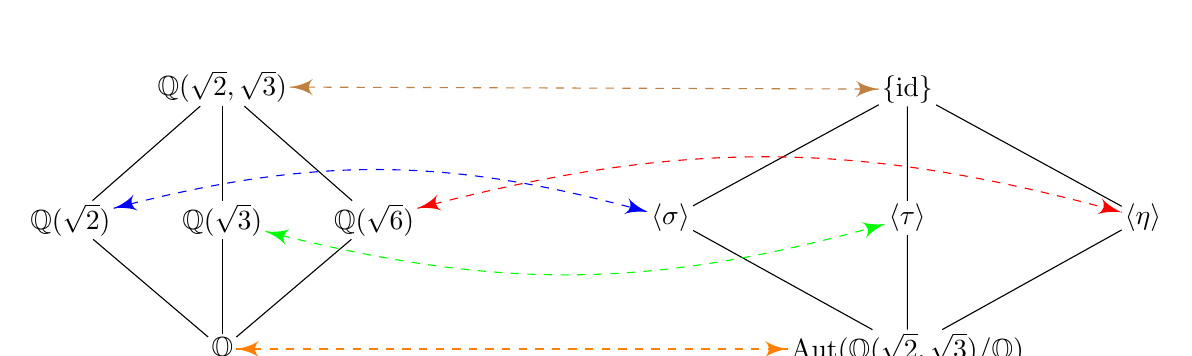
\begin{tikzpicture}[
            node distance=1.2cm and 1.2cm,
            every node/.style={inner sep=1pt},
            correspondence/.style={dashed, <->},
            scale=0.8
          ]

            \node (Q)                        {$\Q$};
            \node[above left=of Q] (Q2)     {$\Q(\sqrt{2})$};
            \node[above right=of Q]      (Q6)     {$\Q(\sqrt{6})$};
            \node[above=of Q] (Q3)    {$\Q(\sqrt{3})$};
            \node[above=of Q3]     (K)      {$\Q(\sqrt{2}, \sqrt{3})$};

            \draw (Q) -- (Q2);
            \draw (Q) -- (Q3);
            \draw (Q) -- (Q6);
            \draw (Q2) -- (K);
            \draw (Q3) -- (K);
            \draw (Q6) -- (K);

            \node[right=7cm of Q]      (Gal)    {$\Aut(\Q(\sqrt{2}, \sqrt{3})/\Q)$};
            \node[above right=of Gal]    (eta)   {$\langle \eta \rangle$};
            \node[above=of Gal]          (tau)    {$\langle \tau \rangle$};
            \node[above left=of Gal]     (sigma)    {$\langle \sigma \rangle$};
            \node[above=of tau]            (G)    {$\set{\id}$};

            \draw (Gal) -- (eta);
            \draw (Gal) -- (tau);
            \draw (Gal) -- (sigma);
            \draw (eta) -- (G);
            \draw (tau) -- (G);
            \draw (sigma) -- (G);

            \draw[correspondence,orange] (Q) -- (Gal);
            \draw[correspondence, bend left=15,blue] (Q2) to (sigma);
            \draw[correspondence, bend right=15,green] (Q3) to (tau);
            \draw[correspondence, bend left=15,red] (Q6) to (eta);
            \draw[correspondence,brown] (K) -- (G);
          \end{tikzpicture}
        \end{center}
  \end{enumerate}
  In this case, $\FF$ and $\GG$ are the inverse
  of each other and invert the containment order.
  Note that the fact these are all the subfield of $\Q(\sqrt{2}, \sqrt{3})$
  follows from (V).
\end{example}

\begin{example}
  \label{exmp:galois-eta}
  Let $\eta \in \C$ be the primitive $5$th root of unity.
  \begin{enumerate}
    \item[(o)]
  We saw in \Cref{exmp:p-one} that $\left[\Q(\eta) : \Q\right] = 4$
  and that
  \[
    \Aut\del{\Q(\eta) : \Q} \cong \del{\Z/5\Z}^{\times} \cong C_4.
  \]
  We will find a generator for $\Aut\del{\Q(\eta)/\Q}$.
  Let $\sigma \in \Aut\del{\Q(\eta) / \Q}$ be the automorphism that satsifies
  $\sigma(\eta) = \eta^2$.
  Such an automorphism must exist since $\eta^2$
  is a root of $\frac{x^5 - 1}{x - 1}$
  which is the minimal polynomial of $\eta$.
  We see that
  \begin{align*}
    \sigma(\eta) &= \eta^2, \\
    \sigma^2(\eta) &= \eta^4, \\
    \sigma^3(\eta) &= \eta^3, \\
    \sigma^4(\eta) &= \eta,
  \end{align*}
  so $\langle \sigma \rangle = \Aut\del{\Q(\eta) / \Q}$.
    \item[(I)]
      We have seen in \Cref{exmp:eta-eta} that
      \[
        \left[\Q(\eta) : \Q(\eta + \eta^{-1})\right] = 2,
      \]
      and thus from
      \[
        4 = \left[\Q(\eta) : \Q\right] =
        \underbrace{\left[\Q(\eta) : \Q(\eta + \eta^{-1})\right]}_{=\,2}
        \left[\Q(\eta + \eta^{-1}) : \Q\right]
      \]
      we get $\left[\Q(\eta + \eta^{-1}) : \Q\right] = 2$,
      so it is a quadratic extension and thus
      there exists a squarefree integer $2 \le r \in \Z$
      so that
      \[
        \Q(\sqrt r) = \Q(\eta + \eta^{-1}).
      \]
    \item[(II)]
      We want to show that $\Q(\sqrt r)$ is the only subfield that is
      properly contained in (not equal) $\Q(\eta)$ which contains $\Q$.

      Let $\Q \subsetneq M \subsetneq \Q(\eta)$.
      Then
      \[
        4 = \left[\Q(\eta) : \Q\right] =
        \underbrace{\left[\Q(\eta) : M\right]}_{1 <}
        \underbrace{\left[M : \Q\right]}_{1 <} \implies
        \left[M : \Q\right] = 2.
      \]
      This implies that there exists a squarefree integer $s \neq 0,1$
      so that $N = \Q(\sqrt s)$ ($s$ may be negative).
      If $s \neq r$, then from the same arguments as in
      \Cref{exmp:galois-q-sqrt-two-sqrt-three} (we didn't use
      the fact that the roots are real)
      we could obtain that $\Aut\del{\Q(\eta) / \Q} \cong C_2 \times C_2$,
      % or at least a subgroup, the isomorphism follows from size
      which is a contradiction.
    \item[(III)] In this case we also get
      that $\FF$ and $\GG$ are the inverse of each other:
      \begin{center}
          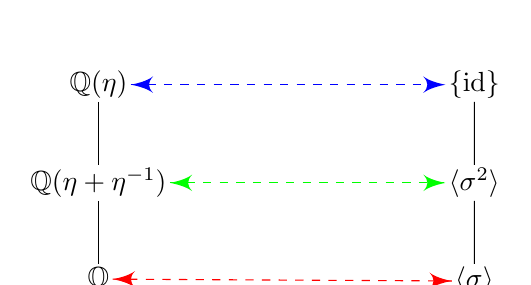
\begin{tikzpicture}[
            node distance=0.8cm and 0.4cm,
            every node/.style={inner sep=1pt},
            field/.style={},
            group/.style={},
            correspondence/.style={dashed, <->},
            scale=0.8
          ]

            \node[field] (Qn)                 {\( \Q(\eta) \)};
            \node[field, below=of Qn] (Qnn)    {\( \Q(\eta + \eta^{-1}) \)};
            \node[field, below=of Qnn] (Q)     {\( \Q \)};

            \draw (Qn) -- (Qnn);
            \draw (Qnn) -- (Q);

            \node[group, right=4cm of Qn] (id)   {$\set{\id}$};
            \node[group, below=of id]  (sig2)   {\( \langle \sigma^2 \rangle \)};
            \node[group, below=of sig2]  (sig)    {\( \langle \sigma \rangle \)};

            \draw (id) -- (sig2);
            \draw (sig) -- (sig2);

            \draw[correspondence,blue] (Qn) -- (id);
            \draw[correspondence,green] (Qnn) -- (sig2);
            \draw[correspondence,red] (Q) -- (sig);
          \end{tikzpicture}
        \end{center}
  \end{enumerate}
\end{example}

\begin{exercise}
  Show that the Galois correspondence induces a bijection between
  the lattice of the subgroups of $\Aut(E/G)$ and the lattice of
  the subfields of $E$ over $\Q$ where $E$ is the splitting field
  of $x^3 - 2$ over $\Q$.
\end{exercise}

\begin{remark}
We have seen examples where $\FF$ and $\GG$ were the inverse of each other
like \Cref{exmp:galois-q-sqrt-two-sqrt-three} and \Cref{exmp:galois-eta},
and examples where they weren't like
\Cref{exmp:galois-correspondence-not-inverse-one}
and \Cref{exmp:galois-correspondence-not-inverse-two}.
We want to figure out what was the difference between these examples.

\begin{itemize}
\item
In \Cref{exmp:galois-q-sqrt-two-sqrt-three} and \Cref{exmp:galois-eta}
the extensions were the splitting fields of polynomials with distinct roots
(all roots were simple - with multiplicity $1$).

\item
In \Cref{exmp:galois-correspondence-not-inverse-one} the extension
$\Q(\sqrt[3]{2}) / \Q$ is not the splitting field of $x^3 - 2 \in \Q[x]$ since
it does not contain the complex roots (although all roots of $x^3 - 2$
\textit{are} distinct/simple).

\item
In \Cref{exmp:galois-correspondence-not-inverse-two}
the extension was $E/F$ where $F$ is of prime characteristic $p$
and $E = F(\alpha)$ for some $\alpha \notin F$ such that $\alpha^p \in F$.
Here $E$ \textit{is} the splitting polynomial of $x^p - a^p$,
but all roots of $x^p - a^p$ are equal - they are not distinct/simple.
\end{itemize}
\end{remark}

\newpage

\section{Separable extensions}
\subsection{Separable polynomials and separable extensions}
\begin{definition}[Simple and multiple roots]
  Let $E/F$ be the splitting field over $F$ of a polynomial
  $0 \neq g(x) \in F[x]$.
  Let $\alpha \in E$ be a root of $g(x)$.
  The multiplicity of $\alpha$ is the maximal value of $k \geq 1$
  so that $(x - \alpha)^k$ divides $g$ (in $E[x]$).
  If the multiplicity of $\alpha$ is $1$ then $\alpha$
  is said to be a simple root.
  Otherwise it is said to be a multiple root.
\end{definition}
\begin{definition}[Separable polynomial]
  Let $F$ be a field and $0 \neq g(x) \in F[x]$.
  Then $g$ is called separable if there exists a splitting field $E/F$
  of $g$ over $F$ so that $g$ doesn't have multiple roots.
\end{definition}

\begin{remark}
  If $g$ is separable with regards to some spliting field,
  then $g$ is separable in all fields in which it splits.
\end{remark}

\begin{definition}[Derivative]
  Let $g(x) = \sum_{i=0}^{n} a_i x^i \in F[x]$ be a polynomial.
  The derivative of $g$ is
  \[
    g'(x) = \sum_{i=1}^{n} i a_i x^{i-1}.
  \]
\end{definition}

\begin{remark}
  If $\char(F) = 0$,
  then $\deg(g') = \deg(p) - 1$.
  If $\char(F) > 0$ the degree might be smaller.
\end{remark}

\begin{example}
  When $g(x) = x^p \in F_p[x]$ we have $g'(x) = p x^{p-1} = 0$.
  Thus $\deg(g) = p$ but $\deg(g') = 0$.
\end{example}

\begin{exercise}
  Show that the derivative is linear.
\end{exercise}
\begin{solution}
  Let $g,h \in F[x]$ be so that $g(x) = \sum_{i=0}^{n} a_i x^i$ and
  $h(x) = \sum_{i=0}^{n} b_i x^i$ and let $c \in F$.
  We have that
  \[
    (cg)'(x) =
    \sum_{i=1}^{n} i c a_i x^{i-1} =
    c \sum_{i=1}^{n} i a_i x^{i-1} =
    c(g')(x)
  \]
  and
  \[
    (g + h)' = 
    \sum_{i=1}^{n} i  (a_i + b_i) x^{i-1} =
    \sum_{i=1}^{n} i a_i x^{i-1} +
    \sum_{i=1}^{n} i b_i x^{i-1} =
    (g)' + (h)'.
  \]
  This shows that the derivative is linear which completes the proof.
\end{solution}

\begin{lemma}
  Let $F$ be a field,
  let $0 \neq g(x) \in F[x]$,
  let $L$ be the splitting field of $g$ over $F$
  and let $\alpha \in L$ be a root of $g$.
  Then $\alpha$ is a multiple root if and only if $\alpha$ is a root
  of $g'$.
\end{lemma}
\begin{proof}
  Let $\alpha = \alpha_1,\dots,\alpha_r$ be the distinct roots of $g$
  in $L$ and let $e_1,\dots,e_r$ be their multiplicities.
  Then there exists $0 \neq C \in F$ so that
  \[
    g(x) = C \prod_{i=1}^{r} (x - \alpha_i)^{e_i},
  \]
  and thus from the product rule:
  \[
    g'(x) =
    C \sum_{i=1}^{r}
    \del{e_i (x - \alpha_i)^{e_i - 1} \prod_{i \neq j} (x - \alpha_j)^{e_j}},
  \]
  and so
  \[
    g'(\alpha) =
    C \sum_{i=1}^{r}
    \del{e_i (\alpha_1 - \alpha_i)^{e_i - 1}
    \prod_{i \neq j} (\alpha_1 - \alpha_j)^{e_j}} =
    C
    \del{e_1 (\alpha_1 - \alpha_1)^{e_1 - 1}
    \prod_{1 \neq j} (\alpha_1 - \alpha_j)^{e_j}}
  \]
  so $g'(\alpha) = 0$ if and only if $e_1 > 1$.
\end{proof}

% Euclid algorithm reminder

\begin{remark}
  Let $g,h \in F[x]$ be polynomials.
  If $E/F$ is a field extension of $F$,
  then when we apply Eulid's algorithm
  we would get the same polynomials in both fields, and thus
  $\gcd(g,h) = r$ in both $F[x]$ and $E[x]$.
\end{remark}

\begin{corollary}
  \label{cor:euclid}
  Let $g,h \in F[x]$ be polynoimals and let $E/F$ be a field extension
  of $F$.
  Then $g$ and $h$ are coprime over $E$ if and only if they are
  coprime over $F$.
\end{corollary}

\begin{exercise}
  \label{ex:coprime-iff-no-common-root}
  Let $F$ be a field and let $h,g \in F[x]$.
  Suppose that $h$ splits in $F$.
  Then $g$ and $h$ are coprime if and only if they don't have a common
  root.
\end{exercise}
\begin{solution}
  Suppose that $g$ and $h$ are coprime.
  Assume, by way of contradiction, that they have a common root $r \in F$.
  Then $(x - r)$ divides both $g$ and $h$ and thus it must divide
  $\gcd(g,h)$ in contradiction to $\gcd(g,h) = 1$.

  Next suppose that $g$ and $h$ don't have a common root.
  Let $\gcd(g,h) = r$.
  Assume, by way of contradiction, that $r \neq 1$.
  Then since $r \mid h$ and $h$ splits in $F$
  we get that $r$ must split in $F$.
  Let $z \in F$ be a root of $r$,
  so that $p := (x - z) \mid r$.
  By properties of $\gcd$ it follows that $p \mid h$ and $p \mid g$
  so they have a common root which is a contradiction.
\end{solution}

\begin{corollary}
  \label{cor:sep-iff-hdh-coprime}
  Let $0 \neq h \in F[x]$.
  Then $h$ is separable if and only if $h$ and $h'$ are coprime
  in $F[x]$.
\end{corollary}
\begin{proof}
  Let $E$ be the splitting field of $h$ over $F$.
  Then by definition
  $h$ is is separable if and only if
  $h$ doesn't have multiple roots.
  Then $h$ doesn't have multiple roots if and only if
  $h$ and $h'$ don't have common roots,
  so combining this with \Cref{ex:coprime-iff-no-common-root}
  we get that $h$ is separable if and only if $h$ and $h'$
  are coprime in $E$.
  From \Cref{cor:euclid} we now get that $h$ is separable if and only if
  $h$ and $h'$ are coprime in $F[x]$.
\end{proof}

\begin{corollary}
  \label{cor:char-zero-implies-irreducible-implies-separable}
  Let $F$ be a field of characteristic $0$.
  Let $h \in F[x]$ be irreducible.
  Then $h$ is separable.
\end{corollary}
\begin{proof}
  Since $h$ is irreducible every divisor of $h$ of degree less than
  $\deg(h)$ is invertible.
  Since $\char F = 0$
  we obtain that $\deg(\gcd(h,h')) \le \deg(h') = \deg(h) - 1 < \deg(h)$,
  so the greatest common divisor of $h$ and $h'$ is invertible.
  Hence $\gcd(h,h') = 1$ so $h$ and $h'$ are coprime.
  Then from \Cref{cor:sep-iff-hdh-coprime} we obtain that $h$ is separable,
  which completes the proof.
\end{proof}

\begin{example}
  \label{exmp:irreducible-and-nonseparable}
  Let $F$ be a field of prime characteristic $p$
  and let $a \in F$ be so that there does not exist $b \in F$
  so that $a = b^p$.
  We have seen in \Cref{ex:show-x-p-irreducible}
  that $h(x) = x^p - a$ is irreducible in $F[x]$.
  Since $h' = 0$ we get that $h$ and $h'$ are not coprime in $F[x]$.
  This shows that $h$ is not separable.
\end{example}

\begin{remark}
  Let $F$ be a field of characteristic $p$.
  We want to understand the polynomials $g \in F[x]$
  which are irreducible and nonseparable.
  Since $g$ is irreducible,
  every polynomial of degree less than $\deg(g)$ that is not
  the zero polynomial is coprime to $g$.
  In particular if $g' \neq 0$ then $g$ and $g'$ are coprime,
  so \Cref{cor:sep-iff-hdh-coprime} implies that $g$ is separable,
  which is a contradiction.
  The implication is that all irreducible and nonseparable
  polynomials $g \in F[x]$ satisfy $g' = 0$, so they must
  be of the form
  \[
    g(x) = \sum_{i=0}^{n} a_i x^{ip}.
  \]
  If we denote $h(x) := \sum_{i=0}^{n} a_i x^i$,
  we can even write $g(x) = h(x^p)$.
  We can even show that $h(x)$ is irreducible.
  Assume, by way of contradiction,
  that there exist $h_1,h_2 \in F[x] \setminus F$ so that
  \[
    h(x) = h_1(x) h_2(x).
  \]
  Then $g(x) = h_1(x^p) h_2(x^p)$
  where both $h_{1,2}(x^p) \in F[x] \setminus F$.
  However, $g$ is irreducible, so we get a contradiction.
  Therefore all irreducible and nonseparable polynomials in a field
  of characteristic $p$ are of the form $g(x) = h(x^p)$
  for some irreducible polynomial $h(x) = \sum_{i=0}^{n} a_i x^i \in F[x]$.
\end{remark}

\begin{proposition}
  \label{prop:irreducible-in-prime-char-fields}
  Let $F$ be a field of a prime characterstic $p$,
  and let $f \in F[x]$ be an arbitrary irreducible polynomial.
  Then there exists a number $e \geq 0$,
  and an irreducible, separable polynomial
  $h(x) \in F[x]$ so that
  \begin{enumerate}
    \item[(1)] $f(x) = h(x^{p^e})$;
    \item[(2)] the multiplicity of each of the roots of $f$ is $p^e$.
  \end{enumerate}
\end{proposition}

\begin{corollary}
  Let $F$ be a field and let $g \in F[x]$ be  irreducible.
  Then any root $r$ in some splitting field of $g$ over $F$
  has has the same multiplicity.
\end{corollary}

\subsection{Finite fields}

\begin{proposition}
  Let $p$ be a prime number.
  Then for all $n \geq 1$ there exists a unique (up to isomorphism)
  field $F$ of order $p^n$.
\end{proposition}
\begin{proof}
  Let $n \geq 1$.
  We have seen that any field of order $p^n$ is isomorphic
  to the splitting field of $x^{p^n} - x$ over $F_p$.
  We now prove existence.
  Denote $h(x) = x^{p^n} - x$.
  Let $E$ be the splitting field of $h(x)$.
  Since $h'(x) = -1$
  we conclude that $h$ and $h'$ are coprime and thus $h(x)$ is separable.
  By definition of seperability we get that
  \[
    L = \set{a \in E \mid h(a) = 0} \subseteq E
  \]
  is a set of cardinality $p^n$.
  Notice that $0,1 \in L$ and that
  it is closed under addition and multiplication,
  since for all $a,b \in L$ we have
  \begin{align*}
    h(a + b) &= (a + b)^{p^n} - (a + b) = a^{p^n} + b^{p^n} - a - b = 0 \\
    h(a \cdot b) &= (a \cdot b)^{p^n} - (a \cdot b) = 0
  \end{align*}
  A nonempty subset of a finite field that contains $0$ and $1$
  and is closed under addition and multiplication is a subfield
  so $L$ is a field of order $p^n$ which completes the proof.
\end{proof}

\begin{remark}
  Notice that since $h(x)$ splits in $L$
  we actually have that $L = E$.
\end{remark}

\begin{definition}[Perfect field]
  A field $F$ is said to be perfect
  if any irreducible polynomial $g(x) \in F[x]$ is separable.
\end{definition}

\begin{example}
  According to \Cref{cor:char-zero-implies-irreducible-implies-separable}
  any field of characteristic $0$ is perfect.
\end{example}

\begin{remark}
  The next proposition shows that any finite field is perfect and 
  any field of rational functions $F(x)$ where $\char(F) = p$
  is not perfect.
\end{remark}

\begin{proposition}
  Let $F$ be a field of charateristic $p > 0$.
  Then $F$ is perfect if and only if the endomorphism of Frobenius
  is surjective.
\end{proposition}
\begin{proof}
  Suppose that $\phi_p$ is not surjective,
  and let $b \in F \setminus \phi_p(F)$.
  We have seen in \Cref{exmp:irreducible-and-nonseparable}
  that $x^p - b$ is irreducible and also nonseparable
  so $F$ is not perfect.

  Next suppose that $\phi_p$ is surjective.
  Let $g(x) \in F[x]$ be irreducible.
  Then from \Cref{prop:irreducible-in-prime-char-fields}
  there exists an irreducible and separable $h(x) \in F[x]$
  and a number $e \geq 0$ so that $g(x) = h(x^{p^e})$.
  Denote $h(x) = \sum_{i=0}^{n} a_i x^i$.
  If we show that $p^e = 1$ then $g(x) = h(x)$
  is separable which completes the proof.
  Since $\phi_p$ is surjective, for all $0 \le i \le n$ there exists
  $b_i \in F$ so that $(b_i)^{p^e} = a_i$.
  We get that
  \[
    g(x) =
    h(x^{p^e}) =
    \sum_{i=0}^{n} a_i x^{i p^e} =
    \sum_{i=0}^{n} \del{b_i x^{i}}^{p^e} =
    \del{\sum_{i=0}^{n} b_i x^{i}}^{p^e},
  \]
  where the last transition follows from the fact $F$ has characteristic
  $p$.
  Since $g(x)$ is irreducible we get that $p^e = 1$, so
  $g(x) = h(x)$ is separable, which completes the proof.
\end{proof}

\begin{remark}
  Every finite field is perfect.
\end{remark}

\subsection{Embeddings of field extensions}

\begin{definition}[Separable element]
  Let $E/F$ be an algebraic field extension.
  Then $\alpha \in F$ is said to be separable over $F$ if
  its minimal polynomial is separable.
\end{definition}

\begin{definition}[Separable extension]
  A field extension $E/F$ is said to be separable if all of its elements
  are separable.
\end{definition}

\begin{example}
  Let $F$ be a field with characteristic $0$.
  Then any algebraic extension of $F$ is separable.
\end{example}

\begin{definition}
  Let $E/F$ be a finite extension,
  let $\varphi \colon F \to \Omega$ be an embedding of $F$ in
  an algebraically closed field $\Omega$.
  Denote
  \[
    i_{\varphi,\Omega}(E/F) =
    \# \set{\hat \varphi \colon E \to \Omega \mid
    \hat \varphi \vert_F = \varphi}.
  \]
\end{definition}

\begin{remark}
  We will soon see that $i_{\varphi,\Omega}(E/F)$
  is not dependent on $\varphi$ or $\Omega$.
  It is only dependent on $E/F$.
\end{remark}

\begin{lemma}
  \label{lem:i}
  Let $E = F(a)$ be a finite simple field extension.
  Let $\Omega$ be an algebraically closed field and let
  $\varphi \colon F \to \Omega$ be an embedding.
  Let $m_a(x) \in F[x]$ be the minimal polynomial of $a$ over $F$.
  Then $i_{\varphi,\Omega}(E/F)$ is equal to the number of different
  embeddings of $E$ in the splitting field of $m_a$ over $F$.
  In particular if $E/F$ is a simple algebraic extension then
  \begin{enumerate}
    \item[(1)] $i_{\varphi,\Omega}(E/F)$ is not dependent on $\varphi$
      or on $\Omega$;
    \item[(2)] $i_{\varphi,\Omega}(E/F) \le [E : F]$;
    \item[(3)] in $(2)$ there is equality if and only if $m_a(x)$
      is separable.
  \end{enumerate}
\end{lemma}
\begin{proof}
  We know that if $\hat \varphi \colon E \to \Omega$ is an extension
  of $\varphi$ then $\hat \varphi(a)$ is a root of $\varphi(m_a)$
  and that the number of different roots of $\varphi(m_a)$ in $\Omega$
  is equal to the number of distinct roots of $m_a(x)$ in the splitting field
  of $m_a$ over $F$.
  \Cref{lem:simple-extension-isomorphism}
  shows that $\hat \varphi$ is determined by the image of $a$ and that
  if $b \in \Omega$ is a root of $\varphi(m_a)$ then $\varphi$ is extendable
  to an embdedding $\hat \varphi \colon E \to \Omega$ so that
  $\hat \varphi(a) = b$.

  Since each embedding is determined by $m_a(a)$,
  which must be a root of $m_a$,
  we immediately get $i_{\varphi,\Omega}(E/F) \le \deg(m_a) = [E : F]$,
  and equality holds if and only if $m_a$ has no multiple roots
  (is seperable).
\end{proof}

\begin{remark}[Intuition for $i(E/F)$]
  We know that $i(E/F)$ is the number of $F$-embeddings of $E$ in
  an algebraic closure of $F$ which we denote $\Omega$.
  For example, the inclusion map $i \colon E/F \to \Omega$
  is always such an embedding (this may be the reason for the notation too).
  In general, if we have a simple field extension $F(a)/F$ (though
  this is true for nonsimple extensions as well),
  for example $\Q(\sqrt[3]{2})/\Q$,
  and we want to understand what $i(\Q(\sqrt[3]{2})/\Q)$ is,
  we first find an algebraically closed field containing $\Q(\sqrt[3]{2})/\Q$,
  for example $\C$.
  Then we notice the most imporatant fact,
  that any $F$-embedding $\sigma$ fixes $F$,
  so it must send roots of the minimal polynomial of $\sqrt[3]{2}$ over $\Q$
  to other roots.
  Therefore, for any $F$-embedding $\sigma$ we obtain
  $\sigma(\sqrt[3]{2}) \in \set{z_1,z_2,z_3}$,
  where $z_1,z_2,z_3$ are the roots of $x^3 - 2$.
  Since $\sigma$ is determined by the value of $\sigma(\sqrt[3]{2})$
  we get $i(\Q(\sqrt[3]{2})/\Q) = 3$.
  Make sure you can visualize the embeddings, each as a union of $\Q$
  and a ``line'' passing through a different root of $x^3 - 2$.
  Make sure you understand why there are $3$ and not $6$ embeddings
  (answer: because we can only send roots to roots).
\end{remark}

\begin{example}
  Since $x^2 + 1$ is separable and $[\C : \R] = 2$
  we can use \Cref{lem:i} to conclude that $i(\C/\R) = 2$,
  which are exactly the identity and complex cojugation (both interchange
  the roots of $x^2 + 1$).
\end{example}

\begin{example}
  Recall \Cref{exmp:aut-of-field-of-char-p}.
  In that case, since any embedding sends a root of
  the minimal polynomial to another root of the minimal polynomial,
  and is determined by it, and the minimal polynomial
  only has one root $t$ we conclude that $i(F_p(t)/F_p(t^p)) = 1$.
  However, $[F_p(t) : F_p(t^p)] = p$,
  because the minimal polynomial of $t$ over $F_p(t^p)$
  is $x^p - t^p = (x - t)^p$ of degree $p$.
  In this case we have $1 = i(F_p(t)/F_p(t^p)) < [F_p(t) : F_p(t^p)] = p$,
  since the point $p$ is a multiple root of the minimal polynomial.
\end{example}

\begin{proposition}
  Let $E/F$ be a finite field extension.
  \begin{enumerate}
    \item[(1)] Let $\varphi_1 \colon F \to \Omega_1$ and
                $\varphi_2 \colon F \to \Omega_2$
                where $\Omega_1$, $\Omega_2$ are algebraically closed.
                Then
                $i_{\varphi_1,\Omega_1} = i_{\varphi_2,\Omega_2}$.
    \item[(2)] If $F \subseteq L \subseteq E$ then
      \[
        i(E/F) = i(E/L) \cdot i(L/F).
      \]
    \item[(3)] $1 \le i(E/F) \le [E : F]$.
  \end{enumerate}
\end{proposition}
\begin{proof} \phantom{}
\begin{enumerate}
  \item[(1) + (2)] The proof is by induction on $[E : F]$
    such that the base case is $[E : F] = 2$ and in this
    case the extension is simple and thus $(1)$ follows from
    the previous lemma (\Cref{lem:i}) and also if
    $F \subseteq L \subseteq E$ then $L = F$ or $L = E$
    and the proposition is trivial.

    Assume that $n = [E : F] > 2$ and we have shown the proposition holds
    for $k < n$.
    Suppose that there does not exist
    a subfield $F \subsetneq L \subsetneq E$
    then $E/F$ is a simple extension and the proof is like in the base case.
    Otherwise, there exists $F \subsetneq L \subsetneq E$.
    For all $1 \le i \le r$ let
    $\varphi_i \colon F \to \Omega_i$ be an embedding of $F$ in an
    algebraically closed field $\Omega_i$.
    For all $1 \le i \le r$ we denote
    \begin{align*}
      A_i &= \set{\hat \varphi \colon L \to \Omega \mid
          \hat \varphi\vert_F = \varphi_i]} \\
      B_i &= \set{\hat \varphi \colon E \to \Omega \mid
          \hat \varphi\vert_F = \varphi_i]}
    \end{align*}
    For all $\psi \in A_i$ we denote
    \[
      C_{\psi,i} = \set{\hat \varphi \colon E \to \Omega \mid
        \hat \varphi\vert_L = \psi]}
    \]
    Then we have
    \[
      B_i = \bigsqcup_{\psi \in A_i} C_{\psi,i}
    \]
    Since $[E : F] > [E : L]$ from the induction hypothesis we know
    that $i_{\psi,\Omega_i}(E/L)$ is independent of $\psi$ and $\Omega_i$
    so we can simply write $i_{\psi,\Omega_i}(E/L) = i(E/L)$.
    Moreover, $|A_i|$ is independent of $\varphi_i$ and $\Omega_i$
    and it is simply equal to $i(L/F)$.
    Then using these observations we get
    \[
      i_{\varphi_i,\Omega_i}(E/F) =
      \sum_{\psi \in A_i} i_{\psi,\Omega_i}(E/L) =
      \sum_{\psi \in A_i} i(E/L) =
      i(E/L) \cdot i(L/F),
    \]
    which completes the proof.
  \item[(3)] Suppose that $E = F(a_1,\dots,a_k)$
    and for all $1 \le j \le k - 1$
    denote $L_j := F(a_1,\dots,a_j)$.
    Then from $(2)$ we obtain that
    \[
      i(E/F) =
      \underbrace{i(E/L_{k-1})}_{\geq 1} \cdots
      \underbrace{i(L_{1}/L)}_{\geq 1} \le
      [E : L_{k-1}] \cdots
      [L_{1} : L] = [E : F],
    \]
    where the inequality follows from \Cref{lem:i}.
    This completes the proof.
\end{enumerate}
\end{proof}

\begin{proposition}
  \label{prop:i}
  Let $E/F$ be a finite field extension.
  Then the following conditions are equivalent:
  \begin{enumerate}
  \item[(1)] There exist $a_1,\dots,a_k \in E$ separable over $F$
    so that $E = F(a_1,\dots,a_k)$.
  \item[(2)] $i(E/F) = [E : F]$.
  \item[(3)] $E/F$ is a separable extension.
  \end{enumerate}
\end{proposition}
\begin{proof} \phantom{}
 \begin{enumerate}
  \item[$(1 \to 2)$] For all $0 \le i \le k$ denote
    $L_i := F(a_1,\dots,a_i)$ and in particular denote $L_0 := F$.
    Since any $a_i$ is separable over $F$, the minimal polynomial 
    of $a_i$ over $F$ denoted by $m_{i,F}$ has no multiple roots.
    Also denote by $m_{i,L_{i-1}}$ the minimal polynomial of $a_i$
    over $L_i$.
    We get that $m_{i,L_{i-1}}$ divides $m_{i,F}$ so it must also have
    no multiple roots.
    Thus each $a_i$ is separable over $L_{i-1}$ so
    \[
      i(E/F) =
      i(E/{L_{k-1}}) \cdots i(L_1/F) =
      [E : L_{k-1}] \cdots [L_1 : F] = [E : F],
    \]
    where the second transition follows from part $(3)$ of \Cref{lem:i}.
  \item[$(2 \to 3)$] Assume, by way of contradiction,
    that there exists $\beta \in E$ which is not separable over $F$.
    Then, from \Cref{lem:i} we get
    \[
      i(E/F) =
      \underbrace{i(E / F(\beta))}_{\le [E : F(\beta)]} \cdot
      \underbrace{i(F(\beta) / F)}_{< [F(\beta) : F]} <
      [E : F(\beta)] \cdot [F(\beta) : F] = [E:F]
    \]
    which is a contradiction to $(2)$ which completes the proof.
  \item[$(3 \to 1)$] Immediate.
  \end{enumerate}
\end{proof}

\begin{corollary}
  The splitting field of a separable polynomial is a separable extension.
\end{corollary}
\begin{proof}
  Let $E$ be a splitting field of a separable polynomial $f \in F[x]$
  and let $a$ be a root of $f$.
  Then the minimal polynomial of $a$ over $F$ is seprable,
  since it divides $f$ which is seprable.
  The result follows since $E = F(a_1,\dots,a_k)$
  where $a_1,\dots,a_k$ are the roots of $f$ in $E$.
\end{proof}

\begin{corollary}
  \label{cor:seperability-of-extensions}
  If $E/L$ and $L/F$ are finite extensions, then $E/F$
  is separable if and only if $E/L$ and $L/F$ are separable.
\end{corollary}
\begin{proof}
  Suppose that $E/F$ is separable.
  If $a \in E$ is seprable over $F$,
  then it is clearly seprable over $L$.
  This implies that $E/L$ and $L/F$ are separable.

  Suppose next that $E/L$ and $L/F$ are separable.
  This implies that
  \[
    [E : F] =
    [E : L] \cdot [L : F] =
    i(E / L) \cdot i(L / F) = i(E / F).
  \]
  Thus from \Cref{prop:i} we get that $E/F$ is separable,
  which completes the proof.
\end{proof}

\begin{exercise}
  Prove \Cref{cor:seperability-of-extensions}
  for $E/L$ and $L/E$ not necessarily finite.
\end{exercise}

\begin{corollary}
  A field is prefect if and only if all of its algebraic extensions
  are separable.
\end{corollary}

\newpage

\section{Normal and Galois extensions}

\subsection{Normal extensions}

\begin{definition}[Normal extension]
  An algebraic field extension $E/F$ is said to be normal if every
  irreducible polynomial (over $F$) which has a root in $E$,
  splits over $E$.
\end{definition}

\begin{example}
  The extension $\Q(\sqrt[3]{2})/\Q$ is not normal
  since the minimal polynomial of $\sqrt[3]{2}$
  has complex roots.
\end{example}

\begin{example}
  The extension $\Q(\sqrt{2})/\Q$ is normal.
\end{example}

\begin{lemma}
  Every finite field extension $E/F$ satisifes
  $\abs{\Aut(E/F)} \le i(E/F)$.
\end{lemma}
\begin{proof}
  Let $\Omega$ be an algebraic closure of $E$.
  Then
  \[
    \Aut(E/F) \subseteq
    \set{\varphi \colon E \to \Omega \mid \varphi\vert_F = \id_F}
  \]
  which is of size $i(E/F)$.
\end{proof}

\begin{remark}
  Geometrically, it is healthy to visualize any element in $\Aut(E/F)$,
  as an $F$-embedding $\sigma$ of $E$ in an algebraically closed $\Omega$,
  such that $\sigma(E) = E$.
  Visualizing is also going to help in the following important proposition.
\end{remark}

\begin{proposition}
  \label{prop:i-normality}
  Let $E/F$ be a finite field extension.
  The following conditions are equivalent:
  \begin{enumerate}
    \item[(1)] $E/F$ is normal.
    \item[(2)] $\abs{\Aut(E/F)} = i(E/F)$.
    \item[(3)] $E$ is the splitting field of some polynomial $g \in F[x]$. 
  \end{enumerate}
\end{proposition}
\begin{proof} \phantom{}
  \begin{enumerate}
    \item[$(1 \to 3)$] Suppose that $E = F(\alpha_1,\dots,\alpha_k)$.
      Denote the minimal polynomial of $\alpha_i$ over $F$
      by $f_i$ for all $1 \le i \le k$.
      Then $f_i$ is irreducible over $F$ and has a root in $E$
      and thus splits in $E$.
      This means that $E$ is the splitting field of the polynomial
      $f_1 \cdot f_2 \cdots f_k$.
    \item[$(3 \to 2)$] Let $\alpha_1,\dots,\alpha_k$ be the roots of $g$.
      In particular $E = F(\alpha_1,\dots,\alpha_k)$.
      Let $\Omega$ be an algebraic closure of $E$.
      It suffices to show that if $\rho \colon E \to \Omega$
      is an embedding such that $\rho_F = \id_F$, then $\rho \in \Aut(E/F)$.
      Since $\rho(g) = g$ we get that
      $\rho$ is a permutation on the roots of $g$,
      and thus
      \[
        \rho(E) =
        \rho\del{F(\alpha_1,\dots,\alpha_k)} =
        F\del{\rho(\alpha_1),\dots,\rho(\alpha_k)} \subseteq E.
      \]
      Moreover,
      \[
        [E : F] =
        \left[\rho(E) : \rho(F)\right] =
        \left[\rho(E) : F\right]
      \]
      and since $\rho(E) \subseteq E$ we get that $\rho(E) = E$
      and therefore $\rho \in (\Aut(E/F))$.
    \item[$(2 \to 1)$]
      Assume, by way of contradiction,
      that there exists $g \in F[x]$ which is irreducible over $F$,
      has a root $\alpha$ in $E$, and does not split over $E$.
      Let $\Omega$ be an algebraic closure of $E$.
      We know that
      \[
        \Aut(E/F) \subseteq
        \set{\varphi \colon E \to \Omega \mid \varphi_F = \id_F},
      \]
      and so in order to get a contradiction it suffices to show
      that there exists $\varphi \colon E \to \Omega$
      so that $\varphi_F = \id_F$ and $\varphi(E) \neq E$.

      Let $\beta \in \Omega \setminus E$ be a root of $g$.
      From \Cref{lem:simple-extension-isomorphism}
      we know that there exists an isomorphism
      $\psi \colon F(\alpha) \to F(\beta)$
      so that $\psi\vert_F = \id$ and $\psi(\alpha) = \beta$.
      We can extend $\psi$ to an embedding $\varphi$ of $E$ in $\Omega$
      (since $1 \le i_{\psi,\Omega}(E/F(\alpha))$).
      Now, $\varphi\vert_F = \psi\vert_F = \id_F$
      but $\varphi(E) \ni \varphi(\alpha) = \psi(\alpha) = \beta$
      which implies that $\varphi(E) \neq E$, and completes the proof.
  \end{enumerate}
\end{proof}

\begin{corollary}
  \label{cor:normal-intermediate-extension}
  Let $E/F$ be a finite normal extension and let $F \subseteq L \subseteq E$
  be an intermediate field.
  Then $E/L$ is normal.
\end{corollary}
\begin{proof}
  There exists $g(x) \in F[x]$ so that $E$ is the splitting field of $g$
  over $F$.
  We know that $E$ is also the splitting field of $f$ over $L$
  and thus $E/L$ is normal.
\end{proof}

\begin{corollary}
  \label{cor:normal-extension-does-not-move}
  Let $F \subseteq E \subseteq L$ be field extensions
  such that $E/F$ is a normal finite extension.
  Then for every $\sigma \in \Aut(L/F)$,
  we have $\sigma(E) = E$.
\end{corollary}
\begin{proof}
  Assume, by way of contradiction,
  that there exists $\sigma \in \Aut(L/F)$ so that $\sigma(E) \neq E$.
  Since $[E : F] = [\sigma(E) : F]$ it is not possible
  that $\sigma(E) \subseteq E$ so there exists $\alpha \in E$
  so that $\sigma(\alpha) \notin E$.
  Let $m_{\alpha}(x) \in F[x]$ be the minimal polynomial of $\alpha$ over $F$.
  Since $m_{\alpha}(x)$ is irreducible and has a root $\alpha \in E$
  and $E/F$ is normal, we get that $m_{\alpha}(x)$ splits in $E$.
  Let $\alpha_1,\dots,\alpha_k \in E$ be the roots of $m_{\alpha}(x)$.
  Since $m_{\alpha}(x) \in F[x]$ and $\sigma \in \Aut(L/F)$ we get that
  \[
    \sigma(m_{\alpha}(\alpha)) = m_{\alpha}(\sigma(\alpha)) = 0,
  \]
    so $\sigma(\alpha)$ is a root of $m_{\alpha}(x)$, but all roots
    of $m_{\alpha}(x)$ are in $E$ so $\sigma(\alpha) \in E$.
    This contradiction completes the proof.
\end{proof}

\begin{example}
  Let $E/F := \Q(i,\sqrt{2})/\Q$ be a finite field extension.
  It is normal with minimal polynomial $m(x) = (x^2 + 1)(x^2 - 2)$,
  and it is also separable as the splitting field of a seprable polynomial.
  From separability we get $i(E/F) = [E : F] = 4$,
  and from normality we get $\abs{\Aut(E/F)} = i(E/F)$,
  and thus $\abs{\Aut(E/F)} = 4$.
  By \Cref{cor:normal-extension-does-not-move},
  we must have $\sigma(i) \in \set{-i,i}$ and
  $\sigma(\sqrt{2}) \in \{\sqrt 2,-\sqrt 2\}$ for all
  $\sigma \in \Aut(E/F)$,
  and therefore these automorphisms form exactly the group $\Aut(E/F)$,
  and it can easily be shown that $\Aut(E/F) = C_2 \times C_2$.
\end{example}

\begin{lemma}
  \label{lem:quadratic-implies-normal}
  Every quadratic field extension is normal.
\end{lemma}
\begin{proof}
  Let $E/F$ be a quadratic field extension.
  That is, $[E : F] = 2$.
  Let $m(x)$ be an irreducible polynomial with a root
  $\alpha \in E \setminus F$.
  Since $E/F$ is quadratic, we have $\deg(m) = 2$ so
  \[
    m(x) = ax^2 + bx + c \in F[x].
  \]
  Now, denote the other root of $m(x)$ by $\alpha'$.
  We know that $\alpha + \alpha' = -b$
  so $\alpha' = -\alpha - b \in E$.
  This means that $m(x)$ splits over $E$ so $E/F$ is normal.
\end{proof}

\begin{question}
  Let $E/L$ and $L/F$ be normal extensions.
  Is $E/F$ necessarily normal?
\end{question}
\begin{answer}
  No!
  Let
  \[
    F := \Q \tand
    L := \Q(\sqrt{2}) \tand
    E := \Q(\sqrt[4]{2}).
  \]
  The extensions $E/L$ and $L/F$ are normal
  since by \Cref{lem:quadratic-implies-normal}
  any quadratic field extension is normal.
  However $E/F$ is not normal since the minimal polynomial of $\sqrt[4]{2}$
  over $F$ is $x^4 - 2$ (irreducible from Eisenstein's criterion),
  and it has a root in $E$, but not all of its roots are in $E$
  since some of them are complex.
  Therefore $E/F$ is not normal.
\end{answer}

\begin{remark}
  Note that when we consider $E/F := \Q(\sqrt[4]{2})/\Q$,
  it becomes very easy to understand it is not a normal extension
  when we visualize things.
  The minimal polynomial of $\sqrt[4]{2}$ is $x^4 - 2$,
  and it has complex roots.
  We can see that we can embed $\Q(\sqrt[4]{2})$ in $\C$
  by sending $\sqrt[4]{2}$ to one of the complex roots,
  so clearly $\abs{\Aut(E/F)} < i(E/F)$,
  so the extension is not normal.
\end{remark}

\subsection{Galois extensions}

\begin{definition}[Galois extension]
  A field extension $E/F$ is said to be a Galois extension
  if it is separable and normal.
\end{definition}
\begin{remark}
  If $E/F$ is a Galois extension
  then the automorphism group $\Aut(E/F)$ is called the Galois group
  of $E/F$ and we denote it by $\Gal(E/F)$.
\end{remark}
\begin{remark}
  Note that a Galois extension is also implicitly required
  to be algebraic, since we require it to be normal.
\end{remark}
\begin{remark}
  Note that if $F \subseteq L \subseteq E$ are fields
  and $E/F$ is a Galois extension,
  then by \Cref{cor:seperability-of-extensions}
  and \Cref{cor:normal-intermediate-extension}
  we get that $E/L$ is a Galois extension.
\end{remark}

\begin{proposition}
  \label{prop:quivalent-galois-conditions-for-finite-extensions}
  Let $E/F$ be a finite field extension.
  Then the following conditions are equivalent:
  \begin{enumerate}
    \item[(1)] $E/F$ is a Galois extension.
    \item[(2)] $\abs{\Aut(E/F)} = i(E/F) = [E : F]$.
    \item[(3)] $E$ is the splitting field of
      a separable polynomial $g \in F[x]$.
  \end{enumerate}
\end{proposition}
\begin{proof} \phantom{}
  \begin{enumerate}
    \item[$(1 \leftrightarrow 2)$]
      We have seen in \Cref{prop:i} and \Cref{prop:i-normality} that
      \[
        1 \le
        \Aut(E/F) \le 
        i(E/F) \le
        [L : K]
      \]
      and that the second inequality is an equality if and only if $E/F$
      is normal, and the third inequality is an equality if and only if $E/F$
      is separable.
      This is the inequality at the center of all things.
    \item[$(3 \to 1)$]
      Let $g \in F[x]$ be a separable polynomial so that $E$ is the splitting
      field of $g$ over $F$.
      Every splitting field is immediately a normal extension.
      If $a$ is a root of $g$ then the minimal polynomial of $a$ over $F$
      divides $g$, and thus that minimal polynomial
      is separable and so $a$ is a separable element.
      Since the extension $E/F$ is generated by roots of $g$,
      and an extension generated by separable elements is separable,
      we conclude that $E/F$ is normal and separable, thus it is Galois.
    \item[$(1 \to 3)$] Assume that $E = F(\alpha_1,\dots,\alpha_k)$
      and for all $1 \le i \le k$ denote $m_i$ the minimal polynomial
      of $\alpha_i$ over $F$.
      Since $E/F$ is seprable we get that $m_i$ is separable.
      Since $E/F$ is normal and $\alpha_i$ is a root of
      the irreducible polynomial $m_i$ then $E$
      contains all roots of $m_i$ for all $1 \le i \le k$.
      By a reordering of the elements we can assume that
      there exists $1 \le j \le k$ so that $m_1,\dots,m_j$
      are distinct and $\set{m_1,\dots,m_k} = \set{m_1,\dots,m_j}$.
      If $1 \le r \neq s \le j$ then $m_r$ and $m_s$ are distinct
      irreducible polynomials over $F$ and thus they don't have a common
      root in $E$.
      We obtain that $E$ is the splitting field of the separable
      polynomial $m_1 m_2 \cdots m_j$.
  \end{enumerate}
\end{proof}

\newpage

\section{The Fundamental Theorem of Galois Theory}

\subsection{A different criterion for a finite Galois extension}

\begin{theorem}[Artin]
  \label{thm:artin}
  Let $E$ be a field and let $G \leqslant \Aut(E)$ be a finite group.
  Denote the fixed field of $G$ by
  $F := \set{x \in E \mid (\forall \sigma \in G) \sigma(x) = x}$.
  Then $[E : F] = \abs{G}$.
\end{theorem}
\begin{proof}
  Since by definition of $F$
  we have that $G \leqslant \Aut(E/F)$ we can immediately obtain that
  $\abs{G} \le [E : F]$.
  It is left to show that $\abs{G} \geq [E : F]$.
  Suppose that $G = \set{\sigma_1,\dots,\sigma_m}$ (so that $\abs{G} = m$).
  We need to show that if $\alpha_1,\dots,\alpha_{m+1} \in E$
  then there exist $x_1,\dots,x_{m+1} \in F$
  not all $0$ so that $\alpha_1 x_1 + \cdots + \alpha_{m+1} x_{m+1} = 0$.
  (this is simply saying that $\alpha_1,\dots,\alpha_{m+1}$
  are linearly dependent over $F$).
  Consider the system of equations:
  \[
    \begin{cases}
      \sigma_1(\alpha_1) x_1 + \cdots + \sigma_1(\alpha_{m+1}) x_{m+1} = 0 \\
      \sigma_2(\alpha_1) x_1 + \cdots + \sigma_2(\alpha_{m+1}) x_{m+1} = 0 \\
      \vdotswithin{
      \sigma_m(\alpha_1) x_1 + \cdots + \sigma_m(\alpha_{m+1}) x_{m+1} = 0} \\
      \sigma_m(\alpha_1) x_1 + \cdots + \sigma_m(\alpha_{m+1}) x_{m+1} = 0
    \end{cases}
  \]
  This system of equations has a nontrivial solutions since there are
  more variables ($x_1,\dots,x_{m+1}$) than equations ($m$ equations).
  Choose a nontrivial solution with the smallest number of nonzero
  coordinates, and denote it $(y_1,\dots,y_k,0,\dots,0)$
  (without loss of generality
  we assume the nonzero entries are the first entries).
  We can multiply this solution by a scalar so that $y_1 = 1$
  so we may assume $y_1 = 1$.
  If $y_2,\dots,y_k \in F$ then the proof is complete.
  We will show that necessarily $y_2,\dots,y_k \in F$
  which will complete the proof.
  Assume, by way of contradiction, that there exists $2 \le j \le k$ so that
  $y_j \in E \setminus F$.
  Without loss of generality $y_2 \in E \setminus F$.
  By definition of $F$
  there exists $\sigma \in G$ so that $\sigma(y_2) \neq y_2$.
  We notice that $(\sigma(y_1),\sigma(y_2),\dots,\sigma(y_k),0,\dots,0)$
  is also a solution to the system of equations,
  since for any $1 \le i \le m$ there exists $1 \le j \le m$
  so that $\sigma^{-1} \sigma_i = \sigma_j$ so
  \begin{align*}
  \sigma_i(\alpha_1) \sigma(y_1) + \cdots +
  \sigma_i(\alpha_{m+1}) \sigma(y_{m+1}) &=
  \sigma\del{\sigma^{-1} (\sigma_i(\alpha_1) \sigma(y_1)) + \cdots +
  \sigma^{-1} (\sigma_i(\alpha_{m+1}) \sigma(y_{m+1}))} \\ &=
  \sigma\del{\sigma^{-1} (\sigma_i(\alpha_1)) y_1 + \cdots +
  \sigma^{-1} (\sigma_i(\alpha_{m+1})) y_{m+1})} \\ &=
  \sigma(\sigma_j(\alpha_1) y_1 + \cdots +
  \sigma_j(\alpha_{m+1}) y_{m+1}) \\ &=
  \sigma(0) = 0.
  \end{align*}
  Thus
  $(y_1 - \sigma(y_1),y_2 - \sigma(y_2),\dots,y_k - \sigma(y_k),0,\dots,0)$
  is also a solution but $y_1 - \sigma(y_1) = 1 - 1 = 0$
  and thus this solution has less than $k$ nonzero entries
  in contradiction to the minimality of $k$.
  This contradiction implies that $y_2,\dots,y_k \in F$.
  This completes the proof.
\end{proof}

\begin{remark}
  If one pictures the lattices of subgroups and subfields as in
  \Cref{exmp:galois-q-sqrt-two-sqrt-three}
  or \Cref{exmp:galois-eta},
  then if $H$ is a subgroup corresponding to a subfield $M$,
  then Artin's theorem shows that $\abs{H}$
  is equal to $[E : M]$,
  and this is true for all corresponding subgroups and subfields.
\end{remark}

\begin{corollary}[Artin's criterion]
  Let $E/F$ be a finite field extension.
  Then $E/F$ is a Galois extension if and only if $F$ is
  the fixed field of $\Aut(E/F)$.
\end{corollary}
\begin{proof}
  Denote the fixed field of $\Aut(E/F)$ by $F \subseteq L \subseteq E$.
  Then
  \[
    L = F \iff
    [E : L] = [E : F] \overset{(1)}{\iff}
    \abs{\Aut(E/F)} = [E : F] \overset{(2)}{\iff}
    E/F \text{ is Galois},
  \]
  where $(1)$ follows from \Cref{thm:artin} and $(2)$
  follows from \Cref{prop:quivalent-galois-conditions-for-finite-extensions}.
\end{proof}

\subsection{The fundamental theorem of Galois theory}

\begin{remark}
  Let $E/F$ be a field extension and denote $G = \Aut(E/F)$.
  Recall we have the Galois correspondence
  \[
  \begin{tikzcd}
    \set{M \mid F \subseteq M \subseteq E \text{ is a subfield}}
    \arrow[r, shift left, "\GG"] &
    \set{H \mid H \leqslant G}
    \arrow[l, shift left, "\FF"].
  \end{tikzcd}
  \]
  with the functions
  \begin{align*}
    &\GG(M) := \Aut(E/M) \leqslant \Aut(E/F) \\
    &\FF(H) := \set{x \in E \mid (\forall \sigma \in H) \sigma(x) = x}.
  \end{align*}
\end{remark}

\begin{theorem}[Fundamental theorem of Galois theory, part A] 
  \label{thm:galois-part-a}
  Let $E/F$ be a finite Galois extension.
  Denote $G = \Gal(E/F)$.
  Then the maps $\FF$ and $\GG$
  are bijections, inverse of each other, and reverse the containment
  order.
  That is,
  \begin{enumerate}
    \item[(1)] For every intermediate field $F \subseteq M \subseteq E$,
      we have that $\FF\del{\GG(M)} = M$.
    \item[(2)] For every subgroup $H \leqslant G$,
      we have that $\GG\del{\FF(H)} = H$.
    \item[(3)] If $M_1 \subseteq M_2$ are intermediate fields,
      then $\GG(M_2) \subseteq \GG(M_1)$.
    \item[(4)] If $H_1 \leqslant H_2$ are subgroups of $G$, then
      $\FF(H_2) \subseteq \FF(H_1)$.
    \item[(5)] If $M = \FF(H)$, then $[E : M] = \abs{H}$.
  \end{enumerate}
\end{theorem}
\begin{proof}
  We have already seen $(3) + (4)$ earlier, and $(5)$ follows from Artin's
  theorem. We will proceed to show $(1)$ and $(2)$.
  \begin{enumerate} 
    \item[(1)] Let $F \subseteq M \subseteq E$ be an intermediate field.
      We know that $M \subseteq \FF(\GG(M))$ so it suffices
      to show that $[E : M] = [E : \FF\del{\GG(M)}]$.
      Indeed,
      \[
        [E : M] \overset{(1)}{=}
        \abs{\Gal(E/M)} \overset{(2)}{=}
        [E : \FF\del{\GG(M)}],
      \]
      where $(1)$ holds since $E/M$ is a finite Galois extension,
      and $(2)$ holds since we know that $\GG(M)$ is finite which means
      we can use Artin's theorem.
    \item[(2)] Let $H \leqslant G$.
    Since $E/F$ is a finite extension,
    its Galois group $G = \Gal(E/F)$ is a finite group,
    and thus $H$ is also finite.
    We know that $H \subseteq \GG\del{\FF(H)}$
    and thus it suffices to show that $\abs{H} = |\GG\del{\FF(H)}|$.
    Indeed,
    \[
      \abs{H} \overset{(1)}{=}
      [E : \FF(H)] \overset{(2)}{=}
      \abs{\Gal(E/\FF(H))} = \abs{\GG\del{\FF(H)}},
    \]
    where $(1)$ follow from Artin's theorem (which is applicable
    since $H$ is finite), and $(2)$ holds since $E/\FF(H)$ is
    a finite Galois extension.
  \end{enumerate}
\end{proof}

\begin{corollary}
  Let $E/F$ be a finite Galois extension and
  let $H \leqslant G = \Gal(E/F)$.
  Denote $M = \FF(H)$.
  Then the degree of the extension $M/F$ is equal to the index of $H$ in $G$
  as groups.
  That is,
  \[
    [M : F] = [G : H].
  \]
\end{corollary}
\begin{proof}
  We have
  \[
    [M : F] =
    \frac{[E : F]}{[E : M]} =
    \frac{\abs{G}}{\abs{H}} =
    [G : H]
  \]
  where the middle equality follows from Artin's theorem,
  which we can apply since $L/M$ and $L/K$
  are finite Galois extensions.
\end{proof}

\begin{lemma}
  \label{lem:lemma-for-galois-part-b}
  Let $E/F$ be a field extension and let $G = \Aut(E/F)$.
  For  all $H \leqslant G$ and all $\sigma \in G$ we have
  $\FF(\sigma H \sigma^{-1}) = \sigma(\FF(H))$.
\end{lemma}
\begin{proof}
  Let $x \in L$.
  Then
  \begin{gather*}
    x \in \FF\del{\sigma H \sigma^{-1}} \\
    \viff \\
    \forall h \in H \quad \sigma h \sigma^{-1}(x) = x \\
    \viff \\
    \forall h \in H \quad h \sigma^{-1} (x) = \sigma^{-1} (x) \\
    \viff \\
    \sigma^{-1}(x) \in \FF(H) \\
    \viff \\
    x \in \sigma\del{\FF(H)}.
  \end{gather*}
\end{proof}

\begin{lemma}
  \label{lem:lemma-for-galois-part-b-two}
  Let $E/F$ be a finite Galois extension with Galois group
  $G = \Gal(E/F)$.
  Let $F \subseteq M \subseteq E$ be an intermediate field
  and denote $H = \GG(M)$.
  Then $M/F$ is normal if and only if for all $\sigma \in G$
  we have $\sigma(M) = M$.
\end{lemma}
\begin{proof}
  We have seen in \Cref{cor:normal-extension-does-not-move}
  that if $E/F$ is a finite field extension (not necessarily Galois)
  and $F \subseteq M \subseteq E$ such that $M/F$ is a normal
  extension then for all $\sigma \in \Aut(E/F)$
  we have $\sigma(M) = M$.

  We now show the opposite direction.
  Assume, by way of contradiction,
  that $M/F$ is not a normal extension
  and let $\Omega$ be an algebraic closure of $E$.
  We have seen in \Cref{prop:i-normality} that when $M/F$ is not normal
  there exists an embedding $\rho \colon M \to \Omega$
  so that $\rho\vert_F = \id$ and $\rho(M) \neq M$.
  We also know that we can extend $\rho$
  to an embedding $\bar \rho \colon E \to \Omega$.
  Since $E/F$ is a finite Galois extension, it is a finite normal extension, so
  we can recall \Cref{cor:normal-extension-does-not-move} and similarly obtain
  that $\bar \rho(E) = E$ and thus $\bar \rho \in \Gal(E/F)$.
  However, now for $\sigma := \bar \rho \in \Gal(E/F)$
  we have that $\sigma(M) = \rho(M) \neq M$, in contradiction to
  what was given.
  This contradiction implies that $M/F$ is a normal extension which
  completes the proof.
\end{proof}

\begin{theorem}[Fundamental theorem of Galois, part B]
  \label{thm:galois-B}
  Let $E/F$ be a finite Galois extension with Galois group
  $G = \Gal(E/F)$.
  Let $F \subseteq M \subseteq E$ be an intermediate field and
  let $H = \GG(M)$.
  Then $M/F$ is a Galois extension if and only if $H$ is normal in $G$.
  Moreover, if $H \normalin G$ then the restriction homomorphism
  $\pi \colon \Gal(E/F) \to \Gal(M/F)$
  which maps $\sigma \mapsto \sigma\vert_M$ is surjective,
  $\ker(\pi) = H$, and there exists an isomorphism 
  which gives $\Gal(M/F) \cong G/H$.
\end{theorem}
\begin{remark}
  Note that in \Cref{thm:galois-B} we have that
  $M/F$ is a Galois extension if and only if $H$ is normal in $G$.
  However since we know that $E/F$ is seperable,
  it follows that $M/F$ is seperable,
  so this statement is equivalent to saying that
  $M/F$ is a normal extension if and only if $H$ is normal in $G$.
\end{remark}

\begin{proofof}{\Cref{thm:galois-B}}
  \begin{gather*}
    H \normalin G \\
    \viff \\
    \forall \sigma \in G \quad \sigma H \sigma^{-1} = H \\
    \viff \mathclap{\hspace{3cm} \text{ by \Cref{thm:galois-part-a}}} \\
    \forall \sigma \in G \quad \FF(\sigma H \sigma^{-1}) = \FF(H) \\
    \viff \mathclap{\hspace{3cm} \text{ by \Cref{lem:lemma-for-galois-part-b}}} \\
    \forall \sigma \in G \quad \sigma(\FF(H)) = \FF(H) \\
    \viff \\
    \forall \sigma \in G \quad \sigma(M) = M \\
    \viff \mathclap{\hspace{3cm} \text{ by \Cref{lem:lemma-for-galois-part-b-two}}} \\
    M/F \text{ is a normal extension}
  \end{gather*}
  Assume that $M/F$ is normal.
  Then clearly $\pi$ is a homomorphism and $\ker(\pi) = H$.
  We have that
  \[
    \abs{\im(\pi)} =
    \abs{G / H} =
    [G : H] \overset{(*)}{=}
    [M : F] =
    \abs{\Gal(M / F)}.
  \]
  where $(*)$ follows from \Cref{thm:galois-part-a}.
  This implies that $\pi$ is surjective.
  From the first isomorphism theorem for groups we get
  $G/H \cong \Gal(M/F)$ which completes the proof.
\end{proofof}

\begin{example}
  Let $E/\Q$ be the splitting field of $x^3 - 2$
  and let $G = \Gal(E/\Q)$.
  Denote $w = e^{2\pi i/3}$ and $\alpha = \sqrt[3]{2}$
  and
  \[
    x_0 = \alpha \qquad
    x_1 = \alpha w \qquad
    x_2 = \alpha w^2.
  \]
  We get the lattices
  \begin{center}
    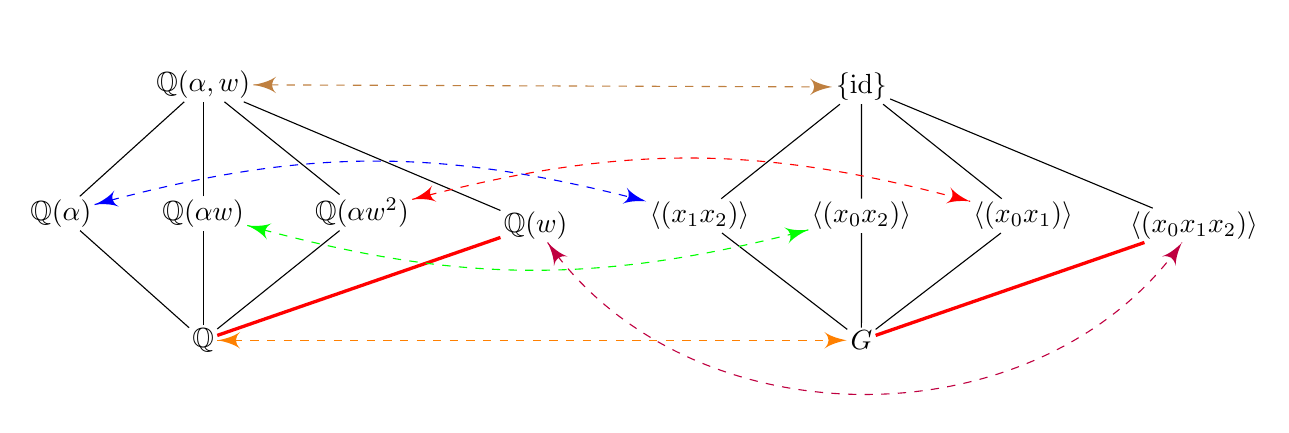
\begin{tikzpicture}[
      node distance=1.2cm and 1.2cm,
      every node/.style={inner sep=1pt},
      correspondence/.style={dashed, <->},
      scale=0.8
    ]

      \node (Q)                        {$\Q$};
      \node[above left=of Q] (Q2)     {$\Q(\alpha)$};
      \node[above right=of Q]      (Q6)     {$\Q(\alpha w^2)$};
      \node[above=of Q] (Q3)    {$\Q(\alpha w)$};
      \node[above=of Q3]     (K)      {$\Q(\alpha,w)$};
      \node[right=4cm of Q]      (mid)    {};
      \node[above=1.2cm of mid]      (w)    {$\Q(w)$};

      \draw (Q) -- (Q2);
      \draw (Q) -- (Q3);
      \draw (Q) -- (Q6);
      \draw (Q2) -- (K);
      \draw (Q3) -- (K);
      \draw (Q6) -- (K);
      \draw[red,very thick] (Q) -- (w);
      \draw (w) -- (K);

      \node[right=8cm of Q]      (Gal)    {$G$};
      \node[above right=of Gal]    (eta)   {$\langle (x_0 x_1) \rangle$};
      \node[above=of Gal]          (tau)    {$\langle (x_0 x_2) \rangle$};
      \node[above left=of Gal]     (sigma)    {$\langle (x_1 x_2) \rangle$};
      \node[above=of tau]            (G)    {$\set{\id}$};
      \node[right=4cm of Gal]      (midgal)    {};
      \node[above=1.2cm of midgal]  (123)  {$\langle (x_0 x_1 x_2) \rangle$};

      \draw (Gal) -- (eta);
      \draw (Gal) -- (tau);
      \draw (Gal) -- (sigma);
      \draw (eta) -- (G);
      \draw (tau) -- (G);
      \draw (sigma) -- (G);
      \draw (123) -- (G);
      \draw[red,very thick] (123) -- (Gal);

      \draw[correspondence,orange] (Q) -- (Gal);
      \draw[correspondence, bend left=15,blue] (Q2) to (sigma);
      \draw[correspondence, bend right=15,green] (Q3) to (tau);
      \draw[correspondence, bend left=15,red] (Q6) to (eta);
      \draw[correspondence,brown] (K) -- (G);
      \draw[correspondence, bend right=55,purple] (w) to (123);
    \end{tikzpicture}
  \end{center}
  where the thick red lines mean that
  $N := \langle (x_0 x_1 x_2) \rangle \normalin G$
  and that $\Q(w)/\Q$ is correpondingly a normal field extension.
  We can see that $G \cong S_3 \cong \Sym(\set{x_0,x_1,x_2})$,
  which implies that $N = A_3$.
  The notation $(x_1 x_2)$ etc.\ is the notation for permutations.
  For example $\langle (x_0 x_1) \rangle$
  is all field automorphisms $\varphi \in \Aut(E/\Q)$ such that exists
  $\sigma \in \langle (x_0 x_1) \rangle$ so that
  $\varphi(x_i) = \sigma(x_i)$.
\end{example}

\begin{corollary}
  \label{cor:constructibles}
  Denote $S_0 = \set{(0,0),(1,0)}$ and let $p$ be an odd prime.
  Then we can construct from $S_0$ a perfect $p$-gon if and only
  if $p$ is a Fermat prime.
\end{corollary}
\begin{proof}
  We have seen in \Cref{exmp:when-pgon-construcible-p-is-fermat}
  that when $p$ is an odd prime
  that the condition that $p$ is a Fermat prime is necessary
  for a $p$-gon to be construcible.
  We will show that this condition is also sufficient.
  Let $p$ be a Fermat prime,
  it suffices to show that $\cos(2\pi/p)$ is constructible.

  Let $\eta \in \C$ be a primitive root of unity of order $p$.
  Thus, we have the identity $\eta + \eta^{-1} = 2\cos(2\pi/p)$.
  We know that $\Q(\eta)/\Q$ is a Galois extension with
  a cyclic Galois group of order $p - 1$.
  Denote $G_0 := \Gal(\Q(\eta) / \Q)$.
  Since $p$ is a Fermat prime there exists a tower of subgroups
  \[
    1 = G_m \leqslant \cdots \leqslant G_1 \leqslant G_0,
  \]
  so that for all $1 \le i \le m - 1$ we have $G_{i-1}/G_{i} = \Z/2\Z$,
  and in particular $[G_{i-1} : G_i] = 2$.
  For all $1 \le i \le m$ denote $\FF(G_i) := F_i$.
  Then from the fundamental theorem of Galois we get that
  \[
    \Q = F_0 \subseteq F_1 \subseteq \cdots \subseteq F_m = \Q(\eta),
  \]
  and from Artin's theorem we get that
  $[F_{i+1} : F_{i}] = 2$ for all $0 \le i \le m - 1$.
  Also, since any cyclic group has at most one cyclic group
  of order $2$, we can conclude that $F_{m-1}$
  is the unique subfield of $\Q(\eta)$ so that $[\Q(\eta) : F_{m-1}] = 2$.
  Since $[\Q(\eta) : \Q(\eta + \eta^{-1})] = 2$
  it follows that $F_{m-1} = \Q(\eta + \eta^{-1})$.
  Recall that $\Q(\eta + \eta^{-1}) = \Q(\cos(2\pi)/p)$,
  so we can write $F_{m-1} = \Q(\cos(2\pi)/p)$.
  Finally, we conclude that there is a tower of fields
  \[
    F_0 \subseteq F_1 \subseteq \cdots
    \subseteq F_{m-2} \subseteq F_{m-1} = \Q(\cos(2\pi)/p)
  \]
  and $[F_{i+1} : F_{i}] = 2$ for all $0 \le i \le m - 2$.
  According to \Cref{thm:constructible-iff-tower-of-fields}
  we get that $\cos(2\pi/p)$ is constructible,
  which completes the proof.
\end{proof}
\begin{remark}
  In \Cref{cor:constructibles}
  we claimed that $[F_{i+1} : F_{i}] = 2$ follows from Artin's theorem
  without explaining too much.
  We will now show a more general claim.
\end{remark}
\begin{proposition}
  Let $E$ be a field and let $1 \leqslant H \leqslant G \leqslant \Aut(E)$
  be finite groups.
  Denote the fixed field of $H$ and $G$ by
  $E^H$ and $E^G$ respectively.
  Then $[E^H : E^G] = \frac{\abs{G}}{\abs{H}} = [H : G]$.
\end{proposition}
\begin{proof}
  By Artin's theorem we have
  $[E : E^H] = \abs{H}$ and $[E : E^G] = \abs{G}$.
  Now we simply have
  \[
    [E^H : E^G] =
    \frac{[E : E^G]}{[E : E^H]} =
    \frac{\abs{G}}{\abs{H}} = [E : G],
  \]
  which completes the proof.
\end{proof}

\newpage

\section{Corollaries from Galois theory}
\subsection{Ruler and compass constructions}
\begin{remark}
  Let $S_0 = \set{(0,0),(1,0)}$.
  We have seen that a $p$-gon (for an odd prime number $p$)
  is constructible if and only if $p$ is a Fermat prime.
  In this section we will generalize this,
  and find a necessary and sufficient condition
  for an $n$-gon to be constructible.
\end{remark}

\begin{definition}[Cyclotomic polynomial]
  Let $\eta \in \C$ be a primitve $n$th root of unity
  for some natural number $n \geq 1$,
  and let $A := \{\eta^d \mid d \in (\Z/n\Z)^{\times}\}$
  be the set of all primitive $n$th roots of unity.
  Then the $n$th cyclotomic polynomial is given by:
  \[
    \Phi_n(x) :=
    \prod_{\alpha \in A}(x - \alpha) =
    \prod_{d \in (\Z/n\Z)^{\times}}(x - \eta^d).
  \]
\end{definition}

\begin{remark}
  Our current goal is to show that $\Phi_n(x) \in \Z[x]$.
\end{remark}

\begin{lemma}
  \label{lem:cyclotomic-polynomials-are-over-z}
  Let $f,g \in \Z[x]$ be polynomials and suppose that $g$ is monic,
  such that $g \mid f$ in $\Q[x]$.
  Then $f/g \in \Z[x]$.
\end{lemma}
\begin{proof}
  We show this by induction on $k = \deg(f) - \deg(g)$.
  If $k = 0$ then $f = \alpha g$ for $\alpha \in \Q$.
  Since $g$ is monic and $f \in \Z[x]$ it follows that $\alpha \in \Z$
  and thus $f/g = \alpha \in \Z[x]$.

  Suppose that $0 < k$ and that we have shown the lemma for values
  less than $k$.
  Write
  \[
    f(x) = a_n x^n + \cdots + a_1 x + a_0
  \]
  so that $a_n \neq 0$.
  Define $h(x) := f(x) - a_n x^k g(x) \in \Z[x]$.
  We have $\deg(h) < n$ and $g \mid h$ in $\Q[x]$.
  Therefore we can use the induction hypothesis to obtain
  \[
    \frac{f}{g} = \frac{a_n x^k g + h}{g} =
    a_n x^k + \frac{h}{g} \in \Z[x].
  \]
\end{proof}

\begin{lemma}
  For all $n \geq 1$ we have $\Phi_n(x) \in \Z[x]$.
\end{lemma}
\begin{proof}
  We will prove this by induction on $n$.
  We have that $\Phi_1(x) = x - 1 \in \Z[x]$.
  Assume that we have shown the lemma for values less than $n > 0$.
  We notice that
  \[
    x^n - 1 =
    \prod_{\substack{\alpha \in \C \\ \alpha^n = 1}} (x - \alpha) =
    \prod_{d \mid n} \Phi_{d}(x) =
    \del[4]{\prod_{\substack{d \mid n \\ d < n}} \Phi_{d}(x)}  \cdot \Phi_n(x).
  \]
  By the induction hypothesis
  $\prod_{\substack{d \mid n \\ d < n}} \Phi_{d}(x)$
  is a monic polynomial in $\Z[x]$,
  and then by \Cref{lem:cyclotomic-polynomials-are-over-z}
  we get that $\Phi_n(X) \in \Z[x]$.
\end{proof}

\begin{exercise}
  \label{ex:polynomials}
  Let $f(x),g(x) \in \Q[x]$ be monic polynomials so that $f \cdot g \in \Z[x]$.
  Then $f,g \in \Z[x]$.
\end{exercise}

\begin{theorem}
  \label{thm:cyclotomic-are-irreducible}
  The cyclotomic polynomials $\set{\Phi_n(x)}_{n=1}^{\infty}$
  are irreducible over $\Q$.
\end{theorem}
\begin{proof}
  Because $\Phi_n(x)$ is monic, Gauss's lemma shows that
  $\Phi_n(x)$ is irreducible over $\Z$ if and only if
  it is irreducible over $\Q$.
  Denote some primitive $n$th root of unity by $\eta$.
  Let $g(x)$ be the minimal polynomial of $\eta$ over $\Q$.
  We want to show that $g = \Phi_n$.
  We know that $g \mid \Phi_n$ over $\Q$
  and that $\Phi_n$ is separable (because $x^n - 1$ is separable).
  Thus since $g$ and $\Phi_n$ are monic,
  it suffices to show that every root of $\Phi_n$ is a root of $g$.
  In other words, we need to show that for each $1 \le d \le n$
  that is coprime to $n$, that $\eta^d$ is a root of $g$.
  Since $d$ is a product of primes (not necessarily different),
  it suffices to show that for any prime $p$ coprime to $n$,
  that $\eta^p$ is a root of $g$ while only using the fact $\eta$
  is a root and a primitive $n$th root of unity.
  Then we could obtain that since $\eta^{p_1}$
  is an $n$th root of unity, and a root of $g$ that $\del{\eta^{p_1}}^{p_{2}}$
  is also a root of $g$, and similarly that
  $n^d = (\eta^{p_1 \cdots p_k}) = \del{\del{\eta}^{p_1}}^{p_2^{\cdots}}$
  is a root of $g$.

  Since $g \mid \Phi_n$ there exists $h(x) \in \Q[x]$ such that
  \[
    \Phi_n(x) = g(x) h(x),
  \]
  so from from \Cref{ex:polynomials} we can
  conclude that $g,h \in \Z[x]$ are monic.
  Let $p$ be a prime that is coprime to $n$.
  We will show that $\eta^p$ is a root of $g(x)$.
  Since $\eta^p$ is a root of $\Phi_n(x)$,
  it must be either a root of $h(x)$ or of $g(x)$.
  Assume, by way of contradiction, that $\eta^p$ is a root of $h(x)$.
  The assumption implies that $\eta$ is a root of $h(x^p)$.
  Thus by definition of $g$ we get that $g(x) \mid h(x^p)$ over $\Q$,
  so by applying \Cref{lem:cyclotomic-polynomials-are-over-z},
  we get that there exists $k(x) \in \Z[x]$ so that
  \[
    h(x^p) = g(x) k(x).
  \]
  If we consider this equation modulu $p$
  (by treating these functions
  as functions $\bar h, \bar g, \bar k \in F_p[x]$),
  we would get the following equation:
  \[
    \del{\bar h(x)}^p =
    \bar h(x^p) =
    \bar g(x) \bar k(x).
  \]
  Since $F_p[x]$ is a principal ideal domain and
  in particular a unit factorization domain,
  there exists a common irreducible factor of $\bar h(x)$ and $\bar g(x)$
  which we will denote by $\bar l(x)$.
  We get that
  \[
    \bar l(x)^2 \mid
    \bar h(x) \bar g(x) =
    \bar \Phi_n(x).
  \]
  This implies that $\bar \Phi_n(x)$ is nonseparable.
  However, $\bar \Phi_n(x) \mid x^n - 1 \in F_p[x]$
  and thus $x^n - 1 \in F_p[x]$ is nonseparable.
  Since $n$ and $p$ are coprime we get that
  \begin{gather*}
    \gcd(x^n - 1,(x^n - 1)') =
    \gcd(x^n - 1,n x^{n-1}) = 1,
  \end{gather*}
  which by \Cref{cor:sep-iff-hdh-coprime} means that $x^n - 1 \in F_p[x]$ 
  is separable so this is a contradiction to $x^n - 1$ being nonseparable.
  This contradiction completes the proof.
\end{proof}



\begin{corollary}
  Let $n \geq 2$ and let $\eta \in \C$ be a primitive $n$th root.
  Then $\Q(\eta)/\Q$ is a Galois extension of degree $\varphi(n)$
  where $\varphi$ is Euler's function,
  and we have $\Gal(\Q(\eta)/\Q) \cong \del{\Z/n\Z}^{\times}$.
\end{corollary}
\begin{proof}
  The extension $\Q(\eta)$ is the splitting field of the separable
  cyclotomic
  polynomial $\Phi_n(x)$ and thus $\Q(\eta)/\Q$ is a Galois extension.
  \Cref{thm:cyclotomic-are-irreducible}
  shows that $\Phi_n(x)$ is irreducible so
  \[
    \abs{\Gal(\Q(\eta)/\Q)} = \left[\Q(\eta) : \Q\right] = \varphi(n) = 
    |(\Z/n\Z)^{\times}|.
  \]
  Define the map $\Phi \colon \Gal(\Q(\eta)/\Q) \to \del{\Z/n\Z}^{\times}$
  by $\Phi(\sigma) = [a] \in \del{\Z/n\Z}^{\times}$
  where $a$ is the exponent of $\eta$ in $\sigma(\eta) = \eta^a$.
  This is a well defined group homomorphism,
  and since $\abs{\Gal(\Q(\eta)/\Q)} = |(\Z/n\Z)^{\times}|$,
  it suffices to show that it is injective.
  Indeed, it is injective since if $\Phi(\sigma) = \Phi(\tau)$
  then $\sigma(\eta) = \tau(\eta)$,
  but since $\sigma,\tau \in \Gal(\Q(\eta)/\Q)$,
  they are determined by their value at $\eta$,
  so $\sigma = \eta$.
  This shows that $\Phi$ is an automorphism and completes the proof.
\end{proof}

\begin{remark}[Group theory reminder]
  \label{rmk:gauss-wantzel}
  Let $p$ be prime and let $G$ be a finite group of order $1 < p^n$.
  Then $Z(G) \neq \set{\id}$ and in particular there exists
  a sequence of normal subgroups
  \[
    \set{\id} = G_0 \normalin G_1 \normalin \cdots \normalin G_m = G
  \]
  so that $[G_i : G_{i-1} = p]$ for all $1 \le i \le m$.
  This is a particular case of the Jordan--H\"older theorem.
\end{remark}

\begin{theorem}[Gauss--Wantzel]
  Let $S = \set{(0,0),(1,0)}$.
  Then we can construct a perferct $n$-gon
  if and only if $n = 2^m \cdot p_1 \cdots p_k$
  for $0 \le m$ and $p_1,\dots,p_k$ are distinct Fermat primes.
\end{theorem}
\begin{proof}
  Denote $\eta := e^{2 \pi i/n}$ so that $2\cos(2\pi/n) = \eta + \eta^{-1}$.
  Recall
  an $n$-gon is constructible if and only if $\cos(2\pi/n)$
  is constructible.
  We know that $\Q(\eta)/\Q$ is an abelian Galois extension
  (its Galois group is abelian),
  so every subgroup $H$ of $\Gal(\Q(\eta)/\Q)$
  is normal, so by the fundamental theorem of Galois
  the fixed field of $H$ is a normal extension of $\Q$.
  In particular $\Q(\cos(2\pi/ n))\Q$ is normal (and it is separable)
  so it is a Galois extension.
  Before continuing we will prove a short lemma.

  \begin{lemma}
    Under the notations of the theorem so far,
    $\cos(2\pi / n)$ if constructible if and only if
    $[\Q(\eta) : \Q]$ is a power of $2$.
  \end{lemma}
  \begin{proof}
  We will start by proving that
  $\cos(2\pi / n)$ is constructible if and only if
  $[\Q(\cos(2\pi/n)) : \Q]$ is a power of $2$.
  One direction follows
  from \Cref{cor:necessary-condition-for-constructability},
  so we will only show that if $\cos(2\pi / n)$ is constructible then
  $[\Q(\cos(2\pi/n)) : \Q]$ is a power of $2$.

  Denote $G := \Gal\del{\Q(\cos(2\pi/n))/\Q}$
  and suppose that $|G| = 2^m$.
  By \Cref{rmk:gauss-wantzel}
  there exists an increasing sequence of normal subgroups
  \[
    \set{\id} = G_0 \normalin G_1 \normalin \cdots \normalin G_m = G,
  \]
  so that $[G_i : G_{i-1} = 2]$ for all $1 \le i \le m$.
  Therefore, by the fundamental theorem
  \[
    \Q = \FF(G_m) \subseteq \FF(G_{m-1}) \subseteq \cdots
    \subseteq \FF(G_0) = \Q(\cos(2\pi/n))
  \]
  is a tower of fields so that $[F_{i} : F_{i-1}] = 2$
  for all $1 \le i \le m$.
  Then by applying \Cref{thm:constructible-iff-tower-of-fields}
  we get that $\cos(2\pi/n)$ is constructible.

  Now since $[\Q(\cos(2\pi/n)) : \Q]$ is a power of $2$ if and only
  if $[\Q(\eta) : \Q]$ is a power of $2$
  (because
  $[\Q(\eta) : \Q(\cos(2\pi/n))] = [\Q(\eta) : \Q(\eta+\eta^{-1})] = 2$),
  we conclude that $\cos(2\pi/n)$ is constructible if and only if
  $[\Q(\eta) : \Q] = \varphi(n)$ is a power of $2$,
  which completes the lemma.
  \end{proof}
  Factorize $n$ into its prime factors
  $n = 2^k \cdot p_1^{s_1} \cdots p_r^{s_r}$,
  and note that since $\varphi$ is multiplicative we get
  \[
    \varphi(n) =
    \varphi(2^k) \cdot \varphi(p_1^{s_1}) \cdots \varphi(p_r^{s_r}).
  \]
  We know that $\varphi(2^k) = 2^{\max\set{k-1,0}}$ so it is always
  a power of $2$.
  We also know that $\varphi(p_i^{s_i}) = (p_i - 1) p_i^{s_i - 1}$.
  Therefore $\varphi(n)$ is a power of two if and only if
  $(p_i - 1) p_i^{s_i - 1}$ is a power of two for all $1 \le i \le r$,
  and this happens if and only if $s_i = 1$ and $p_i$ is a Fermat
  prime for all $1 \le i \le r$.
  This completes the proof.
\end{proof}

\subsection{Simple extensions and the primitive element theorem}
\begin{theorem}
  \label{thm:finite-fields-extensions-are-simple-iff-finite-amount-of-intermediate-fields}
  A finite field extension $E/F$ is simple if and only if it has a finite
  amount of intermediate fields.
\end{theorem}
\begin{proof}
  Assume that $E/F$ has a finite amount of intermediate fields.
  We will show that $E/F$ is simple.
  If $F$ is finite, then $E$ is finite,
  and thus the multiplicative group of $E$ is cyclic
  (see \Cref{cor:multiplicative-group-of-finite-field-is-cyclic}).
  If $\alpha$ is a generator of $E^{\times}$ then $E = F(\alpha)$.
  Therefore, we may assume that $F$ is infinite.
  Since $E/F$ is generated by a finite amount of elements over $F$
  it suffices to show that if $\alpha, \beta \in E$ then there exists
  $\gamma \in E$ so that $F(\alpha,\beta) = F(\gamma)$.
  For every $\delta \in F$ we know that $F(\alpha + \delta \beta)$
  is an intermediate field of the extension.
  Since $F$ is infinite, there exist distinct $\delta_1, \delta_2 \in F$
  so that $L := F(\alpha + \delta_1 \beta) = F(\alpha + \delta_2 \beta)$.
  If we denote $\gamma_i := \alpha + \delta_i \beta$
  for $i = 1,2$ then by a simple arithmetic calculation we can obtain that
  \[
    \beta = \frac{\gamma_2 - \gamma_1}{\delta_2 - \delta_1} \in L,
  \]
  and thus clearly also $\alpha \in L$
  and so $L = F(\gamma_1) = F(\alpha,\beta)$ which completes this part
  of the proof.

  Assume next that $E = F(\alpha)$ is a simple extension.
  Let $g(x) \in F[x]$ be the minimal polynomial of $\alpha$ over $F$.
  We will show that there exists an injective map from the set of intermediate
  fields of $E/F$ to the set of monic polynomials that divide $g(x)$,
  which is a finite set, which will complete the proof.
  Let $F \subseteq L \subseteq E$ be an intermediate field.
  Let $h \in L[X]$ be the minimal polynomial of $\alpha$ over $L$.
  Write it by
  \[
    h(x) = x^m + b_{m-1} x^{m-1} + \cdots + b_0.
  \]
  Notice that since $E = L(\alpha)$ we have that $[E : L] = m$.
  Denote $M := F(b_{m-1},\dots,b_0)$.
  Clearly $M \subseteq L$.
  However, $h(x) \in M[x]$ is irreducible and $E = M(\alpha)$.
  Therefore $[E : M] = m$.
  Thus we must have $M = L$.
  We conclude that every intermediate field $F \subseteq L \subseteq E$
  is generated by the coefficients of a monic polynomial in $E[x]$
  that divides $g(x)$.
  Thus the map that sends each intermediate field to its corresponding
  polynomial is injective which completes the proof.
\end{proof}

\begin{lemma}
  \label{lem:primitive-element-theorem}
  Let $E/F$ be a finite separable extension.
  Then there exists a field $E \subseteq M$ such that $M/F$ is a finite
  Galois extension.
\end{lemma}
\begin{proof}
  Let $E = F(\alpha_1,\dots,\alpha_k)$ and let $g_i$
  be the minimal polynomial of $\alpha_i$ over $F$.
  Denote by $M$ the splitting field of $g = h_1h_2 \cdots h_l$
  over $F$ where $\set{g_1,\dots,g_k} = \set{h_1,\dots,h_l}$
  for distinct $h_i$.
  Then $M$ is a normal extension.
  We also have that $M$ is separable
  since the roots of $g$ are separable and $M$
  is finitely generated over $F$ by the roots of $g$.
\end{proof}

\begin{corollary}[Primitive element theorem]
  Every finite separable field extension is simple.
  In particular, every finite extension of a field of characteristic zero
  is simple.
\end{corollary}
\begin{proof}
  Let $E/F$ be a finite separable extension.
  Let $E \subseteq M$ be so that $M/F$ is a finite Galois extension
  (by \Cref{lem:primitive-element-theorem}).
  Then $\Gal(M/F)$ is finite so it must have a finite amount of subgroups.
  From fundamental theorem of Galois theory, $M/F$ has a finite amount
  of intermediate fields, which means that $E/F$
  has a finite amount of intermediate fields, so by
  \Cref{thm:finite-fields-extensions-are-simple-iff-finite-amount-of-intermediate-fields}
  $E/F$ is a simple extension.
\end{proof}

\begin{example}
  The simplest nonsimple algebraic extension is $K(x,y)/K(x^p,y^p)$
  where $K$ is an algebraically closed field of characteristic $p$.
  We notice that $[K(x,y) : K(x^p,y^p)] = p^2$ since a basis
  for $K(x,y)$ over $K(x^p,y^p)$ is given by the set
  \[
    A := \set{x^i y^j \middle\vert 0 \le i,j \le p-1}
  \]
  and $\abs{A} = p^2$.
  However, for each $\alpha \in K(x,y)$
  we notice that $\alpha^p \in K(x^p,y^p)$.
  This implies that $[K(x^p,y^p)(\alpha) : K(x^p,y^p)] \le p$,
  which means that it is not a simple extension.
  Then by the primitive element theorem
  we conclude that $K(x,y)/K(x^p,y^p)$ is nonsimple.
\end{example}

\subsection{The fundamental theorem of algebra}
\begin{lemma}
  \label{lem:R-has-no-nontrivial-extensions-of-odd-degree}
  The set of real number $\R$ does not have nontrivial extensions
  of an odd degree.
\end{lemma}
\begin{proof}
  Assume, by way of contradiction, that $E/\R$ is of an odd degree
  and let $\alpha \in E/\R$.
  Then
  \[
    \left[\R(\alpha) : \R\right] = \deg(m_{\alpha})
  \]
  is odd.
  Therefore there exists an irreducible polynomial over $\R$ of
  an odd degree $p(x)$.
  Since $\deg(p)$ is odd it has a real root so it must be reducible.
  This contradiction completes the proof.
\end{proof}

\begin{lemma}
  Let $f \in \C[x]$ be a polynomial of degree $2$.
  Then $f$ has a root in $\C$.
\end{lemma}
\begin{proof}
  Follows immediately from the quadratic formula
  and the fact every $\alpha \in \C$ has a root
  (otherwise the quadratic formula was not always defined).
\end{proof}

\begin{corollary}
  \label{cor:C-has-no-extensions-of-degree-two}
  The field of complex numbers $\C$ does not have extensions of degree $2$
\end{corollary}


\begin{theorem}[First Sylow theorem, reminder]
  Let $G$ be a finite group, let $p$ be a prime number,
  and let $m$ be the maximal natural number so that $p^m \mid |G|$.
  Then $G$ has a subgroup of order $p^m$.
\end{theorem}

\begin{theorem}[Fundamental theorem of algebra]
  The field of complex numbers is algebraically closed.
\end{theorem}
\begin{proof}
  First we will show that every $f(x) \in \R[x]$ splits in $\C$.
  Let $f(x) \in \R[x]$ and let $E$ be the splitting field of
  $(x^2 + 1) f(x)$ over $\R$.
  Since $i \in E$ the embedding $\R \hookrightarrow E$ extends
  to an embedding of $\C$ in $E$.
  We identify $\C$ as a subfield of $E$.
  The extension $E/\R$ is normal (since it is a splitting field)
  and it is separable since $\char(\R) = 0$.
  Therefore $E/\R$ is a finite Galois extension.
  Denote $G := \Gal(E/\R)$.
  Then we have that $2 = [\C : \R] \mid [E : \R] = \abs{G}$.
  Let $P$ be a $2$-Sylow subgroup of $G$ and denote $M = \FF(P)$.
  Since $P$ is $2$-Sylow we get that $[G : P] = [M : \R]$ is odd,
  but since by \Cref{lem:R-has-no-nontrivial-extensions-of-odd-degree} $\R$
  doesn't have nontrivial extensions of an odd degree,
  we get that $[G : P] = 1$ so $G = P$.

  Recall that we want to show that $E = \C$
  and from Galois correspondence it is equivalent
  to showing that $H := \GG(\C) = \set{\id}$.
  Assume, by way of contradiction, that $1 < \abs{H}$.
  Since $H \leqslant P$ it is a $2$-group (its order is a power of $2$)
  which is nontrivial, so it has a subgroup $K \leqslant H$ of index $2$.
  Now we get
  \[
    2 = [H : K] =
    [\FF(K) : \FF(H)] =
    [\FF(K) : \C],
  \]
  which is a contradiction to \Cref{cor:C-has-no-extensions-of-degree-two}.
  This completes the proof that every $f(x) \in \R[x]$ splits in $\C$.

  Next we will show that any $f \in \C[x]$ splits in $\C$.
  Let $f(x) \in \C[x]$.
  Then $f \cdot \bar f \in \R[x]$.
  It follows from what we have shown that $f \cdot \bar f$ splits over $\C$,
  and in particular $f$ splits over $\C$.
  This completes the proof.
\end{proof}

\newpage

\section{Solving equations using radicals}
\subsection{Radical extensions and Dedekind's lemma}
\begin{definition}[Galois group of a polynomial]
  Let $F$ be a field,
  and let $g(x) \in F[x]$ be a separable polynomial.
  Then the Galois group of $g$ is defined to be $G_f := \Gal(E_f/F)$,
  where $E_f$ is the splitting field of $g$.
\end{definition}

\begin{remark}
  A finite Galois extension $E/F$ is said to be abelian
  or cyclic if $\Gal(E/F)$ is cyclic or abelian respectively.
\end{remark}

\begin{definition}[Radical extension]
  A finite field extension $E/F$ is said to be a radical extension if there
  exist positive natural numbers $m_1,\dots,m_k$
  and elements $a_1,\dots,a_k \in E$ so that
  $E = F(a_1,\dots,a_k)$ and for all $1 \le i \le k$
  we have that $a_i^{m_i} \in F(a_1,\dots,a_{i-1})$.
\end{definition}

\begin{example}
  The extension $\Q(\sqrt[3]{2})/\Q$ is a radical extension.
\end{example}

\begin{remark}
  It is possible for $E/F$ to be a finite simple radical extension,
  so that there does not exist $a \in E$ so that $E = F(a)$ and
  $a^k \in F$ for some positive natural $k$.
  We will see this in the following example.
\end{remark}

\begin{example}
  Consider the extension $\Q(\sqrt[3]{2},\sqrt[3]{3})/\Q$.
  Since $\char(\Q) = 0$ this extension is separable,
  and since it is finitely generated, by the primitive element
  theorem it must be simple.
  We can also verify easily that it is a radical extension.
  However, there does not exist an element $a \in \Q(\sqrt[3]{2},\sqrt[3]{3})$
  so that $\Q(\sqrt[3]{2},\sqrt[3]{3}) = \Q(a)$
  and $a^k \in \Q$ for some positive natural $k$.
  That is because the Galois group of $\Q(\sqrt[3]{2},\sqrt[3]{3})$
  is isomorphic to $C_3 \times C_3$,
  and the Galois group of $\Q(a)$ would have to be isomorphic to $C_9$.
  We will see this in the following theorem
\end{example}

\begin{theorem}
  \label{thm:galois-of-simple-radical-is-cyclic}
  Let $F$ be a field that contains a primitive $n$th root of unity
  and let $E = F(\alpha)$ be a simple extension such that $\alpha^n \in F$.
  Then $E/F$ is a cyclic Galois extension of an order that divides $n$.
\end{theorem}
\begin{proof}
  Let $\eta \in F$ be a primitive $n$th root of unity.
  Then
  \[
    g(x) :=
    \prod_{1 \le i \le n} (x - \eta^i \alpha) =
    x^n - \alpha^n \in F[x]
  \]
  and $E$ is the splitting field of $g$ over $F$ so $E/F$ is a normal
  extension.
  Since $g$ is separable we conclude that $E/F$ is a Galois extension.

  Now for all $\sigma \in \Gal(E/F)$,
  we have that $\sigma(\alpha)$ is a root of $g(x)$,
  so there exists $1 \le i \le n$ so that $\sigma(\alpha) = \alpha \eta^i$.
  We get that there exists a map
  $\varphi \colon \Gal(E/F) \to \langle \eta \rangle$
  defined by $\varphi(\sigma) = \sigma(\alpha)/\alpha$.
  Since for any $\sigma,\tau \in \Gal(E/F)$ 
  so that $\varphi(\sigma) = \eta^i$ and $\varphi(\tau) = \eta^j$ we have that
  $\varphi(\sigma \tau) = \varphi(\sigma) \varphi(\tau) = \eta^{i + j}$,
  we get that $\varphi$ is a homomorphism.
  Moreover, $\varphi$ is injective since $\sigma$ is determined by
  the image of $\alpha$ (recall that $\sigma \in \Gal(E/F)$ and $E = F(\alpha)$).
  From the first isomorphism theorem we get that $\Gal(E/F)$
  is isomorphic to $\im(\varphi)$ which is a subgroup of $\langle \eta \rangle$
  Thus $\Gal(E/F)$ is a cyclic group of an order that divides $n$.
\end{proof}

\begin{exercise}
  Using the notation from \Cref{thm:galois-of-simple-radical-is-cyclic}
  show that if $m$ is the minimal positive natural number
  so that $\alpha^m \in F$ then $[E:F] = m$.
\end{exercise}

\begin{lemma}[Dedekind's lemma]
  Let $F$ be a field, let $G$ be a group, and
  let $\chi_1,\dots,\chi_k$ be distinct homomorphisms from $G$ to $F^{\times}$.
  Then $\chi_1,\dots,\chi_k$ are linearly independent over $F$.
  That is, if $a_1,\dots,a_k \in F$ and for all $g \in G$
  we have
  \[
    a_1 \chi_1(g) + \cdots + a_k \chi_k(g) = 0,
  \]
  then $a_1 = \cdots = a_k = 0$.
\end{lemma}
\begin{proof}
  We prove this by induction over $k$.
  When $k = 1$ the lemma is obvious.
  Assume that $k \geq 2$ and that we have shown the proposition
  for all values $n < k$.
  Let $a_1,\dots,a_k \in F$ so that for all $g \in G$
  we have
  \[
    a_1 \chi_1(g) + \cdots + a_k \chi_k(g) = 0.
  \]
  We need to show that $a_1 = \cdots = a_k = 0$.
  By the induction hypothesis we may assume that all of the coefficients
  $a_1,\dots,a_k$ are nonzero so in particular $a_2 \neq 0$.
  Since $\chi_1 \neq \chi_2$ there exists $h \in G$ so that
  $\chi_1(h) \neq \chi_2(h)$.
  Thus for all $g \in G$ we have
  \[
    0 = a_1 \chi_1(h g) + \cdots + a_k \chi_k(h g) =
    a_1 \chi_1(h)\chi_1(g) + \cdots + a_k \chi_k(h)\chi_k(g).
  \]
  We now subtract from the equation the equation
  \[
    0 = \chi_1(h)\del{a_1 \chi_1(g) + \cdots + a_k \chi_k(g)},
  \]
  so that for all $g \in G$ we get
  \[
    0 =
    a_2(\chi_2(h) - \chi_1(h)) \chi_2(g) + \cdots
    a_k(\chi_k(h) - \chi_1(h)) \chi_k(g).
  \]
  However this is a contradiction to the induction hyposthesis
  since $\set{\chi_2,\dots,\chi_k}$
  is a linearly independent set of size $k - 1$.
  This contradiction implies
  in particular that $a_2(\chi_2(h) - \chi_1(h)) = 0$
  but since $\chi_1(h) \neq \chi_2(h)$ we can divide
  by $\chi_2(h) - \chi_1(h)$ and get that $a_2 = 0$.
  This completes the proof since as we mentioned at the beginning of the
  proof if $a_2 = 0$ the induction hypothesis immediately implies that
  $a_1 = a_3 = \cdots a_k = 0$ as well.
\end{proof}

\begin{theorem}
  Let $F$ be a field that contains a primitive $n$th root of unity,
  and let $E/F$ be a cyclic Galois extension of order $n$.
  Then there exists $\alpha \in E$ so that $E = F(\alpha)$
  and $\alpha^n \in E$.
\end{theorem}
\begin{proof}
  Let $\eta \in F$ a primitive $n$th root of unity.
  Let $\sigma \in \Gal(E/F)$ so that $\langle \sigma \rangle = \Gal(E/F)$.
  We will first show that there exists $\alpha \in E$
  so that $\sigma(\alpha) = \alpha \eta^{-1}$.
  Notice that for all $\tau \in \Gal(E/F)$ the restriction of $\tau$
  to $E^{\times}$ is a homomorphism from $E^{\times}$ to $E^{\times}$.
  From Dedekind's lemma we get that
  \[
    \sum_{i=1}^{n} \eta^i \sigma^i \neq 0.
  \]
  Thus there exists $\gamma \in E^{\times}$ so that we can define
  \[
    \alpha :=
    \sum_{i=1}^{n} \eta^i \sigma^i(\gamma) \neq 0.
  \]
  Now,
  \[
    \sigma(\alpha) =
    \sum_{i=1}^{n} \sigma(\eta^i) \sigma^{i+1}(\gamma) \overset{\eta \in F}{=}
    \sum_{i=1}^{n} \eta^i \sigma^{i+1}(\gamma) =
    \eta^{-1} \sum_{i=1}^{n} \eta^{i + i} \sigma^{i+1}(\gamma) =
    \eta^{-1} \alpha.
  \]

  We will now show that the minimal polynomial of $\alpha$ over $F$
  is $x^n - \alpha^n$ (in particular $\alpha^n \in F$)
  and that $E = F(\alpha)$.
  
  For all $1 \le i \le n$,
  \[
    \sigma(\alpha^i) =
    \sigma(\alpha)^i =
    \alpha^{i} \eta^{-i}
  \]
  so in particular $\sigma(\alpha^n) = \alpha^n$
  and in particular when $1 \le i \le n$ we have
  \[
    i = n \iff
    \alpha^i \in F = \FF(\langle \sigma \rangle) = \mathrm{Fix}(\sigma).
  \]
  This means that $x^n - \alpha^n \in F[x]$ so it suffices to show
  that $x^n - \alpha^n$ is irreducible to show that it is the minimal
  polynomial of $\alpha$.
  Every monic polynomial of degree $1 \le d < n$ that divides $g(x)$
  is of the form
  \[
    g(x) =
    (x - \alpha \eta^{i_1}) \cdots (x - \alpha \eta^{i_d}) =
    x^d + \cdots + \alpha^d \cdot \eta^j \notin F[x]
  \]
  since $\alpha^d \notin F$ and $\eta^j \in F$.
  Since the minimal polynomial of $\alpha$ over $F$
  necessarily divides $g(x)$ and is in $F[x]$
  it must be equal to $g(x)$.
\end{proof}

\begin{definition}[Commutator]
  Let $G$ be a group, and let $g,h \in G$.
  The commutator of $g$ and $h$ is
  the element
  \[
    [g,h] := g^{-1} h^{-1} g h.
  \]
\end{definition}
\begin{remark}
  The element $[g,h]$ is equal to the group's
  identity if and only if $g$ and $h$ commute,
  hence it is called the commutator of $g$ and $h$.
\end{remark}

\begin{definition}[Commutator subgroup]
  Let $G$ be a group.
  The commutator subgroup (or the derived group) of $G$
  is defined to be the subgroup \textit{generated} by
  all commutators of $G$ and we denote it by $[G,G]$.
\end{definition}
\begin{remark}
  We also define the following recursive sequence of groups
  \[
    G^{(0)} := G \qquad
    G^{(1)} := [G,G] \qquad
    G^{(2)} := [G^{(1)},G^{(1)}] \qquad \cdots \qquad
    G^{(k+1)} := [G^{(k)},G^{(k)}],
  \]
  and so on.
\end{remark}

\begin{exercise} \phantom{}
  \begin{enumerate}
    \item[(1)] Show that $G^{(1)} \normalin G$ and that $G/G^{(1)}$ is abelian.
    \item[(2)] Show that if $N \normalin G$ and $G/N$ is abelian
      then $G^{(1)} \leqslant N$.
  \end{enumerate}
\end{exercise}

\begin{definition}[Solvable group]
  A group $G$ is said to be solvable if here exists a subgroup series
  \[
    1 = G_k \leqslant G_{k-1} \leqslant \cdots \leqslant G_1 \leqslant G_0 = G
  \]
  so that for all $0 \le i < k$ we have
  $G_{i+1} \normalin G_i$ and $G_{i}/G_{i+1}$ is abelian.
\end{definition}

\begin{exercise}
  Let $G$ be group.
  \begin{enumerate}
    \item[(1)] Let $G$ be a solvable group.
      Show that for all $0 \le i \le k$ we have $G^{(i)} \leqslant G_i$.
    \item[(2)] Show that $G$ is solvable if and only if $G^{(k)} = 1$
      for some natural $k$.
    \item[(3)] Let $G$ be a group and let $N \normalin G$.
      Show that $G$ is solvable if and only if $G/N$ and $N$
      are solvable.
  \end{enumerate}
\end{exercise}

% \begin{remark}
%   Let $E/F$ be a Galois extension and let $G := \Gal(E/F)$ be finite.
%   Suppose we have a sequence of subgroups
%   \[
%     1 = G_k \normalin G_{k-1} \normalin \cdots \normalin G_1 \normalin G_0 = G.
%   \]
%   Then we have a sequence
%   \[
%     F = \FF(G_0) \subseteq \FF(G_1) \subseteq \cdots
%       \subseteq \FF_{G_{k-1}} \subseteq \FF(1) = E,
%   \]
%   so that $\FF(G_n)$ is a normal extension of $\FF(G_{n-1})$.
%   Therefore
%   % https://q.uiver.app/#q=WzAsNSxbMSwwLCJcXEdhbChcXEZGKEdfaSkvXFxGRihHX3tpLTF9KSkiXSxbMSwxLCJcXEdhbChFL1xcRkYoR197aS0xfSkpIl0sWzIsMSwiXFxHR1xcZGVse1xcRkYoR197aX0pfSJdLFswLDEsIkdfe2ktMX0iXSxbMiwwLCJHX3tpLTF9L0dfe2l9Il0sWzEsMCwiXFxyaG9faSIsMl0sWzAsNCwiXFxjb25nIiwyXSxbMywxLCI9Il0sWzEsMiwiPSJdXQ==
%   \[\begin{tikzcd}[ampersand replacement=\&,cramped]
%     \& {\Gal(\FF(G_i)/\FF(G_{i-1}))} \& {G_{i-1}/G_{i}} \\
%     {G_{i-1}} \& {\Gal(E/\FF(G_{i-1}))} \& {\GG\del{\FF(G_{i})}}
%     \arrow["\cong"', from=1-2, to=1-3]
%     \arrow["{=}", from=2-1, to=2-2]
%     \arrow["{\rho_i}"', from=2-2, to=1-2]
%     \arrow["{=}", from=2-2, to=2-3]
%   \end{tikzcd}\]
%   and $\ker(\rho_i) = G_i$.
%   Therefore $G$ is solvable if and only if there exists a tower of fields
%   \[
%     F = F_0 \subseteq F_1 \subseteq \cdots \subseteq F_k = E
%   \]
%   so that for all $1 \le i \le k$, the extension $F_i / F_{i-1}$
%   has a cyclic Galois group.
%   All that's left to show is that this extension includes the $n$ primitive
%   root and is normal. %\Cref
% \end{remark}

\subsection{Radical extensions and solvable Galois groups}
\begin{lemma}
  Let $F$ be a field, let $F \subseteq \Omega$ be an algebraically
  closed field, let $g \in F[x]$ and let
  $E := F(\alpha_1,\dots,\alpha_k) \subseteq \Omega$ be a splitting
  field of $g$ over $F$.
  Suppose that $F \subseteq L \subseteq \Omega$ is an intermediate field.
  Then $L(\alpha_1,\dots,\alpha_k)$ is a splitting field of $g$ over $L$
  and the restriction map
  $\rho \colon \Gal(L(\alpha_1,\dots,\alpha_k)/L) \to \Gal(E/F)$
  is injective.
\end{lemma}
\begin{proof}
  It is clear that $L(\alpha_1,\dots,\alpha_k)$ is a splitting field
  of $g$ over $L$.
  Let $\sigma \in \Gal(L(\alpha_1,\dots,\alpha_k)/L)$.
  Then $\sigma\vert_F = \id_F$ and since $E/F$ is normal we get
  that $\im(\sigma_E) \subseteq E$
  so we can conclude that $\sigma\vert_E \in \Gal(E/F)$
  (since $\sigma$ is an $F$-embedding of $E$ into $\Omega$,
  by defintion of normality $\im(E) \subseteq E$).
  Thus $\rho$ is well defined and it is easy to verify that
  it is a homomorphism.
  In order to show that $\rho$ is injective we will show that
  $\ker(\rho) = \set{\id}$.
  Suppose that $\rho(\sigma) := \sigma\vert_E = \id_E \in \Gal(E/F)$. 
  In particular we get that
  $\sigma\vert_{\set{\alpha_1,\dots,\alpha_k}} =
  \id\vert_{\set{\alpha_1,\dots,\alpha_k}}$
  which means that $\sigma$ fixes no only the elements of $L$ (by definition)
  but it also fixes $\alpha_1,\dots,\alpha_k$,
  so clearly $\sigma = \id_L$.
\end{proof}

\begin{lemma}
  \label{lem:solvable-groups}
  Let $F$ be a field and let $E/F$ be a separable radical extension.
  Then $E$ is contained in a radical Galois extension of $E$.
\end{lemma}
\begin{proof}
  Since $E/F$ is a radical extension,
  by definition we have
  \[
    F := F_0 \subseteq F_0(\alpha_1) \subseteq F_1(\alpha_2) \subseteq \cdots
    \subseteq F_{k-1}(\alpha_k) = E
  \]
  where we denote $F_0 := F$ and $F_n := F_{n-1}(\alpha_n)$,
  such that $\alpha_i^{r_i} \in F_{i-1}$ for all $1 \le i \le k$.
  Let $m_i$ be the minimal polynomial of $\alpha_i$ over $F$,
  let $\Omega$ be an algebraic closure of $E$,
  and let $L \subseteq \Omega$ be a splitting field of
  $m_1m_2 \cdots m_k$ over $F$.
  Then since $L$ contains $\alpha_1,\dots,\alpha_k$ we get $E \subseteq L$.
  We notice that $L$ is contained in any normal extension of $F$ that contains
  $E$ (since such an extension contains $\alpha_1,\dots,\alpha_k$
  and thus the roots of $m_1$,$m_2$,\dots,$m_k$).
  Let $E \subseteq M \subseteq L$ be a normal extension of $F$
  which is maximal with respect to containment.
  We want to show that $M = L$.
  Assume, by way of contradiction, that $M \neq L$,
  then there exists $\sigma \in \Gal(L/F)$ and $1 \le i \le k$
  so that $\sigma(\alpha_i) \notin M$.
  Let $1 \le j \le k$ be the minimal index so that $\sigma(\alpha_j) \notin M$.
  We know that $\alpha_j^{r_j} \in F(\alpha_1,\dots,\alpha_{j-1})$
  (if $j = 0$ then $F(\alpha_1,\dots,\alpha_{j-1}) = F$).
  Thus
  $\sigma(\alpha_j)^{r_i} \in F(\sigma(\alpha_1),\dots,\sigma(\alpha_{j-1}))$
  (since $\sigma\vert_F = \id_F$) and
  $F(\sigma(\alpha_1),\dots,\sigma(\alpha_{j-1})) \subseteq M$ from
  minimality of $M$.
  We get that
  \[
    F \subseteq M \subseteq M(\sigma(\alpha_j)).
  \]
  These are both radical extensions,
  so $M(\sigma(\alpha_j)) / F$ is a radical extension that strictly
  contains $M$, which is a contradiction.
  This contradiction completes the proof.
\end{proof}

\begin{definition}[Solvable in radicals]
  Let $F$ be a field and let $g(x) \in F[x]$.
  Then $g$ is said to be solvable in radicals if there exists
  a radical extension $E/F$ so that $g$ splits in $E$.
\end{definition}

\begin{theorem}
  Let $F$ be a field of characteristic $0$.
  Let $h \in F[x]$.
  Then $h$ is solvable in radicals if and only if $G_h$
  is solvable.
\end{theorem}
\begin{proof}
  Let $\Omega$ be an algebraic closure of $F$.
  Denote the Galois group of $h$ by $G_h$.
  Suppose that $G_h$ is solvable and denote $n := (\deg h)!$.
  Let $\eta \in \Omega$ be a primitive $n$th root of unity,
  let $L := F(\eta)$,
  and let $M$ be the splitting field of $h$ over $L$.
  \Cref{lem:solvable-groups} shows that
  $\Gal(M/L)$ has an embedding in $\Gal(E/F)$ and thus is solvable.
  In particular there exists a sequence
  \[
    1 \normalin G_k \normalin G_{k-1} \normalin \cdots \normalin G_o = G
  \]
  so that for all $1 \le i \le k$ we have that $G_{i-1}/G_i$ is cyclic.
  For all $1 \le i \le k$ we denote $L_i = \FF(G_i)$.
  From the fundamental theorem of Galois we get that
  \[
    L = L_0 \subseteq L_1 \subseteq \cdots \subseteq L_k = M.
  \]
  Additionaly, $G_i = \Gal(M/L_i)$ for all $0 \le i \le k$.
  Since $G_i \normalin G_{i-1}$,
  part $B$ of the fundamental theorem of Galois implies that for all
  $1 \le i \le k$ that $L_i$ is a normal extension of $L_{i-1}$,
  and
  \[
    \Gal(L_i/L_{i-1}) \cong G_{i-1} / G_i.
  \]
  and thus $L_i/L_{i-1}$ is a cyclic Galois extension.
  Now since $M$ is the splitting field over $L$ of a polynomial
  of degree $n$,
  \[
    [L_i : L_{i-1}] \mid [M : L] \mid n!.
  \]
  Since $L$ containes the primitive $n!$th root of unity
  it containes a primitive root of unity of order $[L_i : L_{i-1}]$.
  Thus from a theorem from the previous lecture there exists
  $\alpha_i \in L_i$ and a natural number $r_i$ so that
  $L_i = L_{i-1}(\alpha_i)$ and $\alpha_i^{r_i} \in L_{i-1}$.
  We get that the sequence
  \[
    F \subseteq \underbrace{F(\eta)}_{L_0}
      \subseteq L_1 \subseteq \cdots \subseteq L_k = m,
  \]
  where $L_k$ is the splitting field of $h$ over $L$
  and thus contains a splitting field of $h$ over $F$.
  This implies that $h$ is solvable in radicals.

  We proceed to show the other direction.
  Denote the splitting field of $h$ over $F$ by $E$
  and suppose that $E$ is containd in a radical extension $M$.
  From \Cref{lem:solvable-groups}
  we can assume that $M$ is a Galois extension of $F$.
  It suffices to show that there exists a Galois extension $L/F$
  so that $M \subseteq L$ and $\Gal(L/F)$ is solvable
  (because $\Gal(E/F)$ is a quotient of $\Gal(L/F)$ and a quotient of 
  a solvable group is solvable).
  Let
  \[
    F = M_0 \subseteq M_1 \subseteq \cdots \subseteq M_k = M
  \]
  where $M_0 := F$ and $M_{n} = M_{n-1}(\alpha_n)$ for $n > 1$
  and $\alpha_i^{r_i} \in M_{i-1}$ for $i \geq 1$.
  A tower of fields implies solvability by radicals.
  Let $\Omega$ be an algebraic closure of $M$
  and let $\alpha_0 \in \Omega$ be a primitive root of unity of order
  \[
    r_0 := r_1 \cdots r_k.
  \]
  Note that the existence of $\alpha_0$ follows from the fact $\char(F) = 0$.
  Define $L = M(\alpha_0)$, so that $L/F$ is a Galois extension.
  That is because if $M$ is the splitting field of the polyomial $m(x)$
  then $L$ is the splitting field of $m(x)(x^r - 1)$.
  % missing diagram may be critical
  We know that $L_0/F$ is an abelian Galois extension with
  a Galois group isomorphic to $(\Z/r_0\Z)^{\times}$.
  Moreover, since for all $1 \le i \le r$
  the field $M_{i-1}$ contains a primitive $r_i$th root of unity,
  it follows that $\Gal(L_i/L_{i-1})$ is cyclic.
  For all $-1 \le i \le k$ denote $G_i = \GG(L_i)$,
  and then from the fundamental theorem of Galois theory,
  for all $0 \le i \le k$ we get $G_i \normalin G_{i-1}$
  and that $G_{i-1}/G_i \cong \Gal(L_i/L_{i-1})$ is abelian.
  This gives us a subnormal sequence
  \[
    1 = G_k \normalin G_{k-1} \normalin \cdots \normalin G_0 \normalin G_{-1}
    = \Gal(L/F),
  \]
  with abelian quotients, and thus $\Gal(L/F)$ is solvable.
\end{proof}

\begin{exercise}
  Show that $A_5$ is simple and not abelian.
  Conclude that it is not solvable.
  Conclude that $S_5$ is not solvable.
  Show that the groups $S_2,S_3,S_4$ are solvable.
\end{exercise}

\begin{remark}
  In order to construct a polynomial
  which is not solvable in radicals, it suffices to construct
  a polynomial with a Galois group that is isomorphic to $S_5$.
\end{remark}

\begin{exercise}
  Show that the only subgroup of $S_5$ that contains a transposition $(ab)$
  and a cycle of length $5$ is $S_5$.
\end{exercise}

\begin{proposition}
  Let $f \in \Q[x]$ be an irreducible polynomial of degree $5$ which
  has exactly $3$ real roots.
  Then the Galois group of $f$ is isomorphic to $S_5$.
  Thus $\Gal(L/F)$ is not solvable.
\end{proposition}

\subsection{Galois groups of polynomials of degree 
  \texorpdfstring{$n \le 4$}{n}}

Let $f(x) \in \Q[x]$ be a separable polynomial of degree $n$ and let
$\alpha_1,\dots,\alpha_n$ be its roots in a splitting field $E$ of $f$.
We know that the action of $G_f := \Gal(E/F)$
on the roots of $f$ induces an embedding
\[
  \rho \colon G_g \hookrightarrow S_n.
\]
We know that $G_f$ is transitive if and only if $f$ is irreducible.
We would like to know when the image of this embedding is contained in $A_n$.

\begin{definition}[Vandermonde product]
  Let $f \in F[x]$ be a polynomial.
  Then the Vandermonde product of $f$
  is defined to be the determinant of its associated Vandermonde matrix
  which is
  \[
    \Delta(f) :=
    \prod_{\scalebox{0.7}{$1 \le i < j \le n$}} (\alpha_i - \alpha_j).
  \]
\end{definition}

\begin{definition}[Discriminant]
  Let $f \in F[x]$ be a polynomial.
  Then its discriminant is defined by
  \[
    \Dif(f) := \Delta(f)^2 =
    \prod_{\scalebox{0.7}{$1 \le i < j \le n$}} (\alpha_i - \alpha_j)^2.
  \]
\end{definition}

\begin{lemma}
  Let $f \in F[x]$ and let $\sigma \in G_f$.
  Then
  \[
    \sigma(\Delta(f)) = \sgn(\sigma) \cdot \Delta(f),
  \]
  and in particular $\sigma(\Dif(f)) = \sigma(\Delta(f))^2 = \Dif(f)$.
\end{lemma}
\begin{proof}
  From multiplicity of the sign and since transpositions of the form
  $\begin{pmatrix} i & i+1 \end{pmatrix}$
  generate $S_n$, it suffices to show the statement in the case
  $\sigma = \begin{pmatrix} i & i+1 \end{pmatrix}$.
  In this case we get,
  \[
    \sigma(\Delta(f)) =
    \del[4]{\prod_{\substack{1 \le j < l \le n \\ (j,l) \neq (i,i+1)}}
      (\alpha_j - \alpha_l)} \cdot (\alpha_{i+1} - \alpha_{i}) =
    -\Delta(f),
  \]
  which competes the proof.
\end{proof}

\begin{corollary}
  The following propositions hold:
  \begin{enumerate}
    \item[(1)] $\Dif(f) \in \FF(G f) = \Q$.
    \item[(2)] $G_f \subseteq A_n$ if and only if $\Delta(f) \in \Q$.
  \end{enumerate}
\end{corollary}

\begin{remark}
  In what follows we show that $\Dif(f)$ is a polynomial in the coefficients
  of $f$.
  We will additionally show how to compute the Galois groups of (almost)
  any polynomial in $\Q[x]$ of degree $n \le 4$.
\end{remark}

\begin{example}[Polynomials of degree $2$]
  Let $f(x) = x^2 + bx + a \in \Q[x]$.
  Denote the roots of $f$ by $\alpha_1$ and $\alpha_2$.
  Then
  \[
    (\alpha_1 - \alpha_2)^2 =
    (\alpha_1 + \alpha^2) - 4 \alpha_1 \alpha_2 =
    (- b)^2 - 4c = b^2 - 4c,
  \]
  where the second transition follows from
  that fact that the sum of the roots is $-b/a$ and $a = 1$.
  This is the exactly the discriminant $\Delta(f)$.
  Now we have that
  \[
    \Delta(f) \notin \Q \iff
    \Dif(f) \notin \Q^2 \iff
    f \text{ is irreducible} \iff
    G_f \text{ transitive} \iff
    G_f = S_2.
  \]
\end{example}

\begin{example}[Polynomials of degree $3$]
  \label{exmp:polynomials-of-degree-three}
  Let $f(x) = ax^3 + bx^2 + cx + d \in \Z[x]$.
  We know that $f$ is reducible over $f$ if and only if it has a rational
  root of the form $\frac{r}{s} \in \Q$ where $\gcd(r,s) = 1$.
  We want to show that we can deduce whether $f$ is irreducible
  Suppose $\frac{r}{s}$ is a root of $f$,
  then $r \mid d$ and $s \mid a$.
  That is because
  \begin{gather*}
    0 = a\del{\frac{r}{s}}^3 + b\del{\frac{r}{s}}^2 + c\del{\frac{r}{s}} + d
    \iff
    0 = ar^3 + br^2s + crs^2 + ds
  \end{gather*}
  (this is the rational root theorem).
  Suppose $f$ is irreducible.
  Then $G_f$ is a isomorphic to a transitive subgroup of $S_3$,
  so $G_f \cong S_3$ or $G_f \cong A_3$.
  We will try to classify these cases.

  By change of a variable $y = rx + s$ and a multiplication by a scalar
  we can assume that $f(x) = x^3 + bx + c$ (a linear change in variables
  does not change the Galois group)
  where $b,c \in \Q$.
  Let $\alpha_1,\alpha_2,\alpha_3$ be the roots of $f$.
  We have
  \[
    \Dif(f) =
    (\alpha_1 - \alpha_2)^2 (\alpha_2 - \alpha_3)^2 (\alpha_3 - \alpha_2)^2 =
    \del{(\alpha_1 - \alpha_2) (\alpha_2 - \alpha_3) (\alpha_3 - \alpha_2)}^2.
  \]
  Notice that
  \[
    (\alpha_1 - \alpha_2) (\alpha_2 - \alpha_3) (\alpha_3 - \alpha_2) =
    \underbrace{\del{\alpha_1^2 \alpha_3 + \alpha_2^2 \alpha_1 + \alpha_3^2 \alpha_2}}_{v} -
    \underbrace{\del{\alpha_1^2 \alpha_2 + \alpha_2^2 \alpha_3 + \alpha_3^2 \alpha_1}}_{u}.
  \]
  Since $\alpha_1 + \alpha_2 + \alpha_3$ is the coefficient of the quadartic
  term we get that $\alpha_1 + \alpha_2 + \alpha_3 = 0$.
  We also know that
    $\alpha_1 \alpha_2 + \alpha_2 \alpha_1 + \alpha_3 \alpha_1 = b$
    and
    $\alpha_1 \alpha_2 \alpha_3 = -c$.
  Notice that
  \[
    u + v =
    \sum_{1 \le i < j \le 3} \alpha_i \alpha_j (\alpha_i + \alpha_j) =
    \sum_{\substack{1 \le i < j \le 3 \\ k \neq i,j}}
    \del{\alpha_i \alpha_j \underbrace{\del{\alpha_i + \alpha_j + \alpha_k}}_{=\,0} - \underbrace{\alpha_i \alpha_j \alpha_k}_{=\,c}} = -3c.
  \]
  Similarly, we can show that $uv = b^3 + 9c^2$.
  Thus
  \[
    \Dif(f) = (v - u)^2 = (v + u)^2 - 4 u v = -27c^2 - 4b^3.
  \]
  This allows us to conclude that
  $G_f \subseteq A_3$ if and only if $\Dif(f) = -27c^2 - 4b^3$
  is a square in $\Q$.
\end{example}

\begin{example}[Polynomials of degree $4$]
  Let $E/\Q$ be a splitting of a polynomial $f \in \Q[x]$
  of degree $4$ which is irreducible.
  Let $\alpha_1,\dots,\alpha_4 \in E$ be the roots of $f$.
  Denote
  \begin{align*}
    u &:= \alpha_1 \alpha_2 + \alpha_3 \alpha_4 \\
    v &:= \alpha_1 \alpha_3 + \alpha_2 \alpha_4 \\
    w &:= \alpha_1 \alpha_4 + \alpha_2 \alpha _3
  \end{align*}
  Since
  \[
    u - v = \alpha_1 (\alpha_2 - \alpha_3) + \alpha_4 (\alpha_3 - \alpha_2) =
    (\alpha_1 - \alpha_4) (\alpha_2 - \alpha_3) \neq 0,
  \]
  we obtain that $u \neq v$,
  and similarly we can show that $u$, $v$, and $w$ are distinct.
  Denote
  \[
    V := \set{\id, (12)(34), (13)(24), (14)(23)}.
  \]
  Then $V \normalin S_4$ and $S_4/V \cong S_3$ (home exercise).
  Denote $M = \Q(u,v,w)$.
  We can verify directly that $\GG(M) = G_f \cap V$.
  Now we can deduce from
  $V \normalin S_4$ that $G f \cap V \normalin G_f$.
  From the fundamental theorem
  of Galois theory $M/\Q$ is a normal extension and
  \[
    \Gal(M/\Q) \cong G_f / \GG(M).
  \]
  Denote $g(x) = (x - u)(x - v)(x - w) \in M[x]$.
  We can express the coefficients of $g(x)$ using the coefficients of $f(x)$
  (home exercise).
  By \Cref{exmp:polynomials-of-degree-three}
  we can find $G_f / \GG(M)$.
  Since $f$ is irreducible, $G_f$ acts transitively,
  and $4 \mid \abs{G_f}$,
  we can simply classifiy all subgroups of $S_4$
  that satisfy these conditions.
  The options are:
  \begin{center}
    \begin{tabular}{c|c|c}
    $G_f$ & $|\GG(M)|$ & $|G_f/\GG(M)| = [M : F]$ \\ \hline
    $S_4$ & $4$            & $6$                          \\ \hline
    $A_4$ & $4$            & $3$                          \\ \hline
    $V$   & $4$            & $1$                          \\ \hline
    $D_4$ & $4$            & $2$                          \\ \hline
    C\_4  & $2$            & $2$                          \\
    \end{tabular}
  \end{center}
  We can conclude that unless $|G_f/\GG(M)| = 2$,
  we can determine $G_f$.
  How can we differentiate between $D_4$ and $C_4$?
  We know that $G_f \cap V$ is transitive if and only if $G_f = D_4$
  if and only if $f \in M[x]$ is irreducible,
  and we will not get into it but there is a way to determine this.
\end{example}

\newpage

\section{Transcendence degree}
\begin{definition}[Algebraically independent elements]
  Let $E/F$ be a field extension.
  We say that $a_1,\dots,a_k \in E$ are algebraically
  independent over $F$ if for all $0 \neq g \in F[x_1,\dots,x_n]$
  we have $g(a_1,\dots,a_n) \neq 0$.
\end{definition}

\begin{example}
  An element $\alpha \in \R$ is algebraically independent if and only if
  it is transcendental.
\end{example}

\begin{remark}
  Notice that if $a_1,\dots,a_k$ are algebraically independent
  then $F(a_1,\dots,a_n) \cong F(x_1,\dots,x_n)$.
\end{remark}

\begin{lemma}
  \label{lem:for-steinz}
  Let $E/F$ be a field extension.
  Let $a_1,\dots,a_{k} \in F$ be algebraically independent over $F$, and
  suppose that $a_1,\dots,a_{k+1} \in F$ are algebraically dependent over $F$.
  Then $\alpha_{k+1}$ is algebraic over $F(a_1,\dots,a_k)$.
\end{lemma}
\begin{proof}
  There exists $0 \neq g \in F[x_1,\dots,x_{k+1}]$
  such that $g(a_1,\dots,a_{k+1}) = 0$.
  Write
  \[
    g = \sum_{i=0}^{m} g_i(x_1,\dots,x_k) x^i_{k+1}.
  \]
  Since $g \neq 0$,
  there exists $0 \le j \le m$ so that $g_j \neq 0$.
  Since $a_1,\dots,a_k$ are algebraically independent over $F$
  we get $g_j(a_1,\dots,a_k) \neq 0$
  and thus
  \[
    0 \neq h(x) =
    \sum_{i=0}^{m} g_i(a_1,\dots,a_k) x^i \in
    F(a_1,\dots,a_k)[x],
  \]
  and $h(a_{k+1}) = 0$,
  which completes the proof.
\end{proof}

\begin{corollary}
  Let $E/F$ be a finitely generated field extension.
  Then if $E/F$ is not an algebraic extension,
  there exist algebraically independent elements $a_1,\dots,a_k \in E$
  so that $E/F(a_1,\dots,a_k)$ is algebraic.
\end{corollary}

\begin{lemma}[Steinitz exchange lemma]
  Let $E/F$ be a finitely generated non algebraic field extension.
  Let $k \in \N^+$ be the minimal number so that there exist
  $a_1,\dots,a_k \in E$ algebraically independent over $F$,
  so that $E/F(a_1,\dots,a_k)$ is algebraic.
  Let $b \in E$ be transcendental over $F$,
  and let $1 \le j \le k$ be minimal so that $a_1,\dots,a_j,b$
  are algebraically dependent over $F$.
  Then $a_1,\dots,a_{j-1},b,a_{j+1},\dots,a_k$ are algebraically
  independent over $F$
  and $E/L$ is algebraic where
  $L = F(a_1,\dots,a_{j-1},b,a_{j+1},\dots,a_k)$.
\end{lemma}
\begin{proof}
  By definition of $j$, we get that $a_1,\dots,a_j,b$
  are algebraically dependent over $F$,
  and that $a_1,\dots,a_{j-1},b$
  are algebraically independent over $F$.
  By \Cref{lem:for-steinz} we conclude that
  $a_j$ is algebraic over $F(a_1,\dots,a_{j-1},b)$.
  We now have that $L(a_j)/L$ and $E/L(a_j)$
  are algebraic extension, and thus $E/L$ is algebraic as well.
  Finally, if $a_1,\dots,a_{j-1},b,a_{j+1},\dots,a_k$
  are algebraically dependent,
  then from the previous lemma we can conclude that
  $L/M$ is algebraic where $M = F(a_1,\dots,a_{j-1},a_{j+1},\dots,a_k)$.
  Since $E/L$ and $L/M$ are algebraic extensions we conclude that
  $E/M$ is an algebraic extension,
  which is a contradiction to the minimality of $k$.
  This contradiction completes the proof.
\end{proof}

\begin{proposition}
  Let $E/F$ be a finitely generated non algebraic field extesnion.
  Let $k \in \N$ be the minimal natural number so that
  there exist $a_1,\dots,a_k \in E$ algebraically independent over $F$
  so that $E/L$ is algebraic where $L = F(a_1,\dots,a_k)$.
  If $b_1,\dots,b_m$ are algebraically dependent then $m \le k$.
  Moreover, $m = k$ if and only if $E/M$ is algberaic where
  $M = F(b_1,\dots,b_m)$.
\end{proposition}
\begin{proof}
  First, we will prove that for all $1 \le j \le \min\set{m,k}$ there
  exist $1 \le i_{1,j} < i_{2,j} < \cdots < i_{k-j,j}$ so that
  $b_1,\dots,b_j,a_{i_{1,j}},\dots,a_{i_{k-j,j}}$
  are algebraically independent over $F$
  and the extension
  $E/F(b_1,\dots,b_j,a_{i_{1,j}},\dots,a_{i_{k-j,j}})$ is algebraic.

  The case $j = 1$ follows from the previous lemma.
  Assume that we have shown the statement for $1 \le j < k$
  and show it for $j + 1$.
  This follows from applying the previous lemma for
  $b_1,\dots,b_j,a_{i_{1,j}},\dots,a_{i_{k-j,j}}$
  and the element $b_{j+1}$.

  We now continue to prove the theorem.
  What we have shown implies that
  \begin{enumerate}
    \item[(1)] $m \le k$ since otherwise $b_{k+1}$ is algebraic over
      $b_1,\dots,b_k$.
    \item[(2)] If $k = m$ then $E$ is algberaic over
      $F(b_1,\dots,b_m)$.
    \item[(3)] If $m < k$ then there exists $1 \le i \le k$
      so that $a_i$ is transcendental over $F(b_1,\dots,b_m)$
      and in particular $E/F(b_1,\dots,b_m)$ is not algebraic.
  \end{enumerate}
  This completes the proof.
\end{proof}

\begin{definition}[Transcendence degree]
  Let $E/F$ be a finitely generated field extension.
  The transcendence degree
  of $E/F$ is the minimal $k$ so that there exist $a_1,\dots,a_k \in E$
  that are algebraically independent over $F$
  so that $E/F(a_1,\dots,a_k)$ is an algebraic extension.
\end{definition}

\begin{definition}[Transcendence basis]
  Let $E/F$ be a finitely generated field extension of
  transcendence degree $k \geq 1$.
  Then any set of $k$ algebraically independent elements over $F$
  so that $E/F(a_1,\dots,a_k)$ is an algebraic extension
  is called a transcendental basis of $E$ over $F$.
\end{definition}

\begin{example}
  \label{exmp:transcendence}
  Let $F$ be a field and let $E = F(x_1,\dots,x_n)$
  be the field of rational functions over $F$ in $n$ variables.
  Then the transcendence degree of $E$ over $F$ is $n$.
  Let $G$ be some subgroup of $S_n$.
  Then we define an embedding $\rho \colon G \to \Aut(E/F)$
  in the following way:
  For each $\sigma \in G$ we define
  \[
    \rho(\sigma)(x_i) := x_{\sigma(i)},
  \]
  for all $1 \le i \le n$.
  Denote $H = \rho(G)$ and $L = \FF(H)$.
  From Artin's theorem it follows that $E/F$ is a Galois extension
  and $\Gal(E/L) \cong H$.
\end{example}

\begin{example}
  Recall \Cref{exmp:transcendence}
  and consider the case $G = S_n$.
  For all $1 \le k \le n$ define:
  \[
    p_1 = \sum_{1 \le i \le n} x_i \qquad
    p_2 = \sum_{1 \le i_1 < i_2 \le n} x_i x_j \qquad
        \cdots \qquad
    p_k = \sum_{1 \le i_1 < \cdots < i_j \le n} x_{i_1} \cdots x_{i_j}
  \]
  Note that for all $\sigma \in S_n$ and for all $1 \le i \le k$
  we have $\rho(\sigma)(p_i) = p_i$.
  Like in \Cref{exmp:transcendence},
  denote $H = \rho(G)$, $L = \FF(H)$, and also denote $M = F(p_1,\dots,p_n)$.
  We have that $M \subseteq L$,
  and we want to show that $L = M$.
  Since the transcendence degree
  of $L$ is $n$, we get that $L$ is isomorphic to $F(x_1,\dots,x_n)$.
  The isomorphism is the map
  $\varphi \colon F(x_1,\dots,x_n) \to F(p_1,\dots,p_n)$
  given by $\varphi(x_i) = p_i$.

  We know that $M \subseteq L$ and that $[E : F] = |S_n| = n!$.
  In order to show that $M = L$ it suffices to show that $[E : M] \le n!$.
  Define
  \[
    M[t] \ni g(t) :=
    t^n - p_1 t^{n-1} + \cdots + (-1)^{n-1} p_{n-1} + (-1)^n p_n =
    (t - x_1) (t - x_2) \cdots (t - x_n).
  \]
  Thus, $E$ is the splitting field of $g$ over $M$,
  and in particular $[E : M] \le n!$.
\end{example}

\begin{exercise}
  Let $E/F$ be an extension of transcendence degree $k$.
  \begin{enumerate}
    \item[(1)] Suppose that $F \subseteq L \subseteq E$
      and $E/L$ is an algebraic extension,
      then the transcendence degree of $L/F$ is $k$.
    \item[(2)] Suppose that $E = F(a_1,\dots,a_k)$ and that $E/F$
      has transcendence degree $k$.
      Then $E$ is isomorphic to the ring of rational functions in $k$
      variables over $F$, and $a_1,\dots,a_k$ form a transcendence basis
      of $E/F$.
  \end{enumerate}
\end{exercise}

% \begin{remark}
%   We have seen that
%   \[
%     \Fix(S_n) = F(p_1,\dots,p_n).
%   \]
%   Thus,
%   \[
%     F[x_1,\dots,x_n] \cap \Fix(S_n) \supseteq F[p_1,\dots,p_n].
%   \]
% \end{remark}
% \begin{exercise}
%   Show that the containment in %\Cref previous remark
%   is actually an equality.
% \end{exercise}

% \begin{corollary}
%   There exists a polynomial $h(t_1,\dots,h_n) \in F[t_1,\dots,t_n]$
%   so that
%   \[
%     \prod_{1 \le i < j \le n} (x_i - x_j)^2 = h(p_1,\dots,p_n)
%   \]
%   where $p_1,\dots,p_n$ are defined like previously in %\Cref
%
%   Thus, if
%   \[
%     l(x) = (t - \alpha_1) \cdots (t - \alpha_n) = t^n + b_{n-1} t^{n-1} + \cdots + b_0
%   \]
%   then
%   \[
%     \Dif(l) = \prod_{1 \le i < j \le n} (\alpha_i - \alpha_j)^2,
%   \]
%   and since each $p_i \in F[x_1,\dots,x_n]$ we can simply
%   choose the variables to be $x_i = \alpha_i$ and then
%   \[
%     \Dif(l) =
%     h(p_1(\alpha_1,\dots,\alpha_n), \dots, p_n(\alpha_1,\dots,\alpha_n)) =
%     h(b_{n-1},\dots,b_{0}).
%   \]
%   This means that the discriminant of a monic polynomial is a polynomial
%   in the coefficients of the polynomial.
%   % this is good in calculation? infi3 recall
% \end{corollary}

% \newpage
%
% \section{Infinite Galois extensions}
%
% Let $p$ be a prime number
% Then
% \[
%   F_p \subseteq F_{p^2} \subseteq F_{p^4} \subseteq \cdots \subseteq F_{p^{2m}}  \subseteq \subseteq \cdots
% \]
% Denote this sequence of fields by $\set{F_n}_{n=1}^{\infty}$ then define
% \[
%   E := \bigcup_{i \geq 1} F_i.
% \]
% We denote $G = \Gal(E / F_1)$. % why is E/F_1 is galois?
%
% \begin{question}
%   How many subfields does $E$ have?
%   Find all subfields %in these notes
% \end{question}
%
% The subfields of $E$ are exactly $\set{F_n}_{n=1}^{\infty}$.
%
% What is $\Gal(E/F_1)$.
%
% We claim that
% there exists $\psi \colon \Gal(E/F_i) \to \prod_{j \geq 1} \Gal(F_j / F_1)$
% so that $\sigma \mapsto (\sigma \mid_{F_j})_j$
%
% We have that $\psi$ is injective.
%
% Show that
% \[
%   \im \psi =
%   \set{(\sigma_j)_j \in \prod_{j \geq 1} \Gal(F_j / F_1) \mid (\forall j_2 > j_1)\sigma_{j_2}\vert_{F_{j_1}} = \sigma_1}.
% \]
%
% Thus $|\Gal(E/F_1)| = 2^{\aleph_0}$
%
% How many subgroups does $\Gal(E/F_1)$ have?
% We know that
% \[
%   \abs{\# \text{cyclic subgroups}} \cdot \aleph_0 \geq 2^{\aleph_0}.
% \]
% Thus there are at least $2^{\aleph_0}$ subgroups,
% and in fact there are exactly $2^{\aleph_0}$ subgroups.
%
% There are $2^{\aleph_0}$ subgroups, and $\aleph_0$ subfields.
% What going on with Galois correspondence?
%
%
% We know that any product of finite sets is a topological compact space
% with respect to the discrete topology
%
% bluh bluh
%
% what's important is that $\im \psi$ is a closed subgroup.
%
% The Galois correspondence is between subfields and closed subgroups.
%
% \newpage
%
% \section{Traces and Norms}
% \subsection{Traces and norms}
% \begin{definition}[Traces]
%   Let $E/F$ be a finite field extension.
%   Then $E$ is a vector field of finite dimension over $F$.
%   An element $a \in E$ defines an $F$-linear map
%   $T_a \colon E \to E$ defined by
%   \[
%     T_a(x) := ax.
%   \]
%   We define
%   \[
%     \tr_{E/F}(a) = \tr(T_a)
%   \]
%   and
%   \[
%     N_{E/F}(a) = \det(T_a).
%   \]
% \end{definition}
%
% \begin{proposition}
%   Denote the characteristic polynomial of $a$ by $C_{E/F,a}(x)$.
%   If $C_{E/F,a} = x^n + a_{n-1} x^{n-1} + \cdots + a_0$,
%   then $\tr(a) = -a_{n-1}$ and $nanika = a_i (-1)^n$.
% \end{proposition}
%
% \begin{remark}
%   The map $\tr \colon E \to F$ is a homomorphism between the additive
%   groups of the field.
% \end{remark}
%
% \begin{remark}
%   The map $N \colon E^{\times} \to F^{\times}$ is a homomorphism
%   between the multiplicative groups of the field.
% \end{remark}
%
% \begin{example}
%   Let $F = \R$ and $E = \C$ and $a = x + yi \in \C$ for some
%   $x,y \in \R$.
%   Let $B = \set{1,i}$ be an ordered basis of $\C$ oover $\R$.
%   Then
%   \[
%     [T_a]_B =
%     \begin{pmatrix}
%       x & -y \\
%       y & x
%     \end{pmatrix}
%   \]
%   and $\tr_{E/F}(a) = 2x$ and $N_{E/F}(a) = x^2 + y^2$.
% \end{example}
%
% \begin{lemma}
%   Let $E/F$ be a finite field extension and let $a \in E$.
%   Denote the minimal polynomial of $a$ over $F$ by $m_a(x)$.
%   Then $C_{E/F,a}(x) = m_a(x)^{[E : F(a)]}$.
% \end{lemma}
% \begin{proof}
%   For every polynomial $g(x) \in F[x]$,
%   we know that $T_{g(a)} = g(T_a)$.
%   Thus the minimal polynomial of $T_a$ is $m_a$ and its degree must be
%   equal to $[F(a) : F]$.
%   In case $E = F(a)$ we get that $m_a(x)$ and $C_{E/F,a}(x)$
%   (which is a monic polynomial that vanishes at $T_a$) are of the same
%   degree and are thus equal.
%
%   In the general case, let $x_1,\dots,x_n$ be a basis for $F(a)/F$
%   and let $y_1,\dots,y_m$ be a basis for $E/F(a)$.
%   Then the representing matrix of $a$ in the basis
%   \[
%     \set{x^i y^j \mid 1 \le i \le n \stand 1 \le j \le m}
%   \]
%   is simply
%   \[
%     \begin{pmatrix}
%       A & & & \\
%         & A & & \\
%       & & & \dots
%     \end{pmatrix}
%   \]
%   where $A$ is the representing matrix of $T_a\vert_{F(a)}$ in basis
%   $x_1,\dots,x_n$.
%   We get that
%   \[
%     C_{E/F(a),a}(x) = m_a(x)^{[E : F(a)]}.
%   \]
% \end{proof}
%
% \begin{corollary}
%   Let $E/F$ be a finite separable field extension
%   and let $\Omega$ be an algebraic closure of $E$.
%   Let $a \in E$, let $\sigma_1,\dots,\sigma_{[F(a) : F]}$
%   be the distinct $F$-embeddings of $F(a)$ in $\Omega$
%   (this means that they fix $F$),
%   and let $\tau_1,\dots,\tau_{E : F}$ be the distinct $F$-embeddings
%   of $E$ in $\Omega$.
%   Then
%   \[
%     T_{?} =
%     \underbrace{[E : F(a)]}_{:=m} \sum_{i} \sigma_i(a) =
%     \sum_{j} T_j(a)
%   \]
%   and
%   \[
%     N_{E/F}(a) = (\prod_i \sigma_i(a)) = \prod_j T_j(a).
%   \]
% \end{corollary}
% \begin{proof}
%   We know that $m_{F,a}(x) = \prod_i (x - \sigma_i(a))$
%   and that the restriction map from the set of $F$-embeddings
%   of $E$ in $\Omega$ to the set of $F$-embeddings
%   of $F(a)$ in $\Omega$ is surjective and $m$-to-$1$.
% \end{proof}
%
% \subsection{Hilbert 90}
%
% \begin{theorem}[Hilbert 90]
%   Let $E/F$ be a cylic finite Galois extension and denote
%   $G := \Gal(E/F) = \langle \sigma \rangle$.
%   Then $x \in E$ satisfies $N_{E/F}(a) = 1$ if and only if
%   there exists $\beta \in E$ so that $a = \frac{\beta}{\sigma(\beta)}$.
% \end{theorem}
% \begin{proof}
%   The norm is a multiplicative homomorphism and we know that
%   \[
%     N_{E/F}(\beta) =
%     \prod_{\tau \in G} \tau(\beta) =
%     \prod_{\tau \in G} \tau(\sigma(\beta)) =
%     N_{E/F}(\sigma(\beta))
%   \]
%   and thus
%   \[
%     N_{E/F}(a) = \frac{N_{E/F}(\beta)}{N_{E/F}(\sigma(\beta))} = 1.
%   \]
%
%   Next suppose that $N_{E/F}(a) = 1$.
%   This implies that $\prod_{\sigma \in G} \sigma(a) = 1$.
%
%   Define a map $f \colon G \to E^{\times}$ in the following way:
%   \[
%     f(\sigma) = a \tand
%     f(\sigma^{i+1}) = f(\sigma) \cdot \sigma(f(\sigma^i)).
%   \]
%   Notice that this map is well defined since $f(\sigma^2) = a \sigma(a)$
%   and $f(\sigma^3) = a \sigma(a) \sigma^2(a)$ and so
%   \[
%     f(\sigma^{n+1}) =
%     a \underbrace{\sigma(a) \cdots \sigma^{n+1}(a)}_{=\, \sigma(N_{E/F}(a)) = 1} = a.
%   \]
%   Now, by Dedekind's lemma
%   the map $\sum_{\tau \in G} f(\tau) \tau \colon E \to E$
%   defined by $a \mapsto \sum_{\tau \in G} f(\tau) \tau(a)$
%   is not the zero map on $E^{\times}$
%   (since each $\tau \colon E^{\times} \to E^{\times}$ is a character
%   and $\sigma \neq a = f(\sigma)$).
%
%   Thus there exists $\beta \in E^{\times}$ so that
%   \[
%     \gamma := \sum_{\tau(a)} f(\tau) \tau(\beta) \neq 0
%   \]
%   and thus,
%   \begin{align*}
%     \sigma(\gamma) &=
%     \sum_{\tau \in G} \sigma(f(\tau)) \sigma \tau(\beta) \\ &=
%     \sum f(\sigma)^{-1} f(\sigma \tau) \sigma \tau(\beta) \\ &=
%     \tau(\sigma) \sigma(f(\tau)) \\ &=
%     f(\sigma)^{-1} \sum_{\tau' \in G} f(\tau') \tau'(\beta) \\ &=
%     f(\sigma)^{-1}  = \alpha^{-1} \gamma.
%   \end{align*}
%
%   We get that
%   \[
%     \sigma(\gamma) = \frac{\gamma}{a} \implies
%     a = \frac{\gamma}{\sigma(\gamma)}.
%   \]
% \end{proof}
%






\end{document}
